\section{Numerical Analysis of Complex LSF Walls-Ambient Conditions}

Finite element method (FEM) is a numerical technique to arrive at a solution for a boundary value problem using partial differential equation to the nearest approximation. The analysis carried out with this methodology is termed as Finite Element Analysis (FEA). FEA works with the logic of minimising the error function in the given boundary value problem by employing variations methods from calculus. Many numerical validation methods prevail till date, but FEM is one of the easiest methods of solving the given problem. The major advantages of using FEM is that any complex problem can be discretised into a simpler problem and analysed in parts to arrive at the result. 

There are many FEA packages commercially available in the market. Packages that are widely used by researchers and engineers are ANSYS, ABAQUS, NASTRAN, PATRAN, LS-Dyna etc. Each package has its own unique features and varies in their utility with respect to time and release of the software patches. The decision to use a specific FEA package depends on the necessity of the end user. ABAQUS is proposed for use in this research for structural FE analysis. ABAQUS originally got its name from the calculation tool abacus. Major modules of the software are CAE (Complete ABAQUS environment), explicit, standard, CFD (Computational Fluid Mechanics) and Electromagnetic. The CAE module is generally used to develop the models in a GUI (Graphical user interface) environment. Other methods of importing the model from other FEA packages are also readily available. Programming languages such as Fortran and Python are embedded within the ABAQUS environment so that the end user is left with endless customization options depending upon their requirements. The standard module in ABAQUS is used for addressing problems related to general structural and multiphysics. As the name suggests the explicit module addresses the contact problems in an efficient manner. The CFD module is used for computational fluid dynamics problems involving liquid flow or thermal flow problems and the Electromagnetic environment is meant for problems related to computational electromagnetics. Since this research focuses on the structural behaviour of LSF walls CAE module will be used for numerical modelling and analysis.

\section{ABAQUS Modelling Set-up}

The numerical models were created in ABAQUS within the CAE environment. Despite the ambient capacity experiments consisting of 4 and 6 studs the numerical models were created with single stud only to achieve maximum computational efficiency. As the stud arrangements are symmetric in the ambient temperature capacity tests of LSF walls, modelling and analysing the single stud was considered as the efficient approach. This consideration was based on past literature on the structural FE models developed by \citet{Shahbazian2011,Gunalan2013f,Kesawan2016a,Ariyanayagam2019}. The FEA simulation for predicting the ambient temperature capacity of double and staggered stud walls comprises of two steps. Firstly, linear buckling analysis was performed on the studs to determine the buckling load under ambient conditions. After determining the buckling load, local imperfections were included in the model (d/150) based on \citet{Gunalan2013f} and static non-linear analysis was carried out to determine the ultimate capacity of LSF wall. The following steps were carried out to determine the buckling load of the studs. As ABAQUS does not have any system of units built in, it is left to the discretion of the user to follow consistent units throughout the model. The International System of Units (SI) was used throughout the modelling and analysis of the complex LSF walls in this research study. The first step was to create the sketch of the lipped channel section (LCS) studs in the GUI windows as shown in \Cref{fig:ABAQUS-sketch}.
\begin{figure}[!htbp]
	\centering
			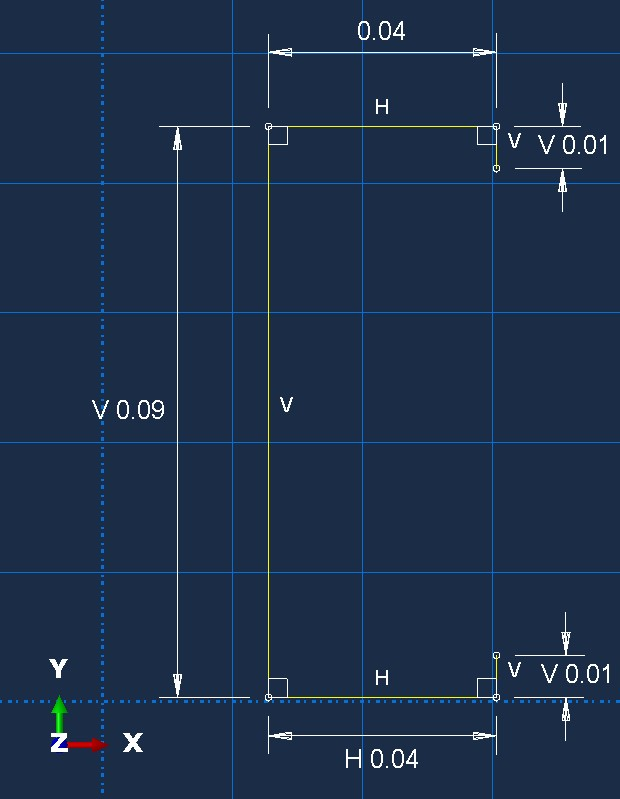
\includegraphics[scale=0.4]{ABAQUS-sketch.jpg}\\
		\caption{Input screen for sketching showing typical LCS stud - ABAQUS }
		\label{fig:ABAQUS-sketch}
\end{figure}

Centreline dimensions were used in the modelling as shell modelling technique was used in the simulation. 3D shell elements were used for the linear buckling and static non-linear analysis under ambient temperature conditions using S4R (4-node shell) element with reduced integration. After completing the section sketch, the model was extruded to 3 m length, depicting studs in the experimental set-up. The extruded section sketch forms a FEATURE in the FE model. The FEATURE forms the PART with additional components and are discussed next. A PART can have single or multiple FEATURES. Some of the additional components of a PART includes, SETS, Section Assignments and Engineering Features such as Inertia and Spring Constants. However, only SETS and Section Assignment will be used in the current structural FE model. For FEA the material properties plays a major role in determining the structural capacity of the developed model. The material properties of steel such as yield stress and elastic modulus were extracted from \citet{Kankanamge2011} which were later confirmed by \citet{Rokilan2019}. The measured yield strength and elastic modulus are entered in the true stress-strain form as Engineering stress-strain curves are not an accepted form of input in the ABAQUS CAE environment. Yield strength of 610 MPa and elastic modulus of 200 GPa were used in the ambient temperature structural analysis. The density of steel was kept constant at 7850 $kg/m^3$. Once the material properties of steel are keyed in, they are assigned to the corresponding PART through Section Assignment. The PART is then imported into the assembly, wherein two independent INSTANCES of the stud are created. Multiple point constraints (MPCs) using beam element were used at the top and bottom of the model on a reference point replicating the centre of gravity (CG) of the model and appropriate boundary conditions were assigned to it. This is achieved by tying all the edges at the top and bottom of the model to their corresponding reference points as shown in \Cref{subfig:abaqus-mpc-contraint}. Translations along the x, y and z-axes were fixed at the bottom of the model while the model was free to move along the z-axis at the top. The model was fixed against rotation along the z-axis only at the top and bottom. Translation along the x-axis was fixed on the stud flanges at screw locations (300 mm) to simulate the lateral restraints provided by plasterboards on the exterior flanges. Individual plasterboards were not modelled to improve the computational efficiency. Lateral restraints provided by the noggings were specified at 1 m intervals on all the flanges. A mesh density of 4 mm was adopted throughout the model based on past literature and initial sensitivity study as shown in \Cref{subfig:abaqus-meshes-structural}. A concentric unit load was applied at the top reference point and the buckling analysis was carried out by specifying linear perturbation in the step option. \Cref{fig:abaqus-full-assembly} shows a typical double stud wall model in ABAQUS. Ten eigen modes were requested for each model to investigate the buckling modes of the studs. The input file was modified with ``*NODE FILE U" argument to collect the buckling modes as a data file and to be used in the non-linear analysis. The buckling analysis results were viewed with the in-built data visualization tool in ABAQUS CAE environment.
\begin{figure}[!htbp]
	\centering
	\begin{subfigure}[b]{0.4\textwidth}
		\centering
		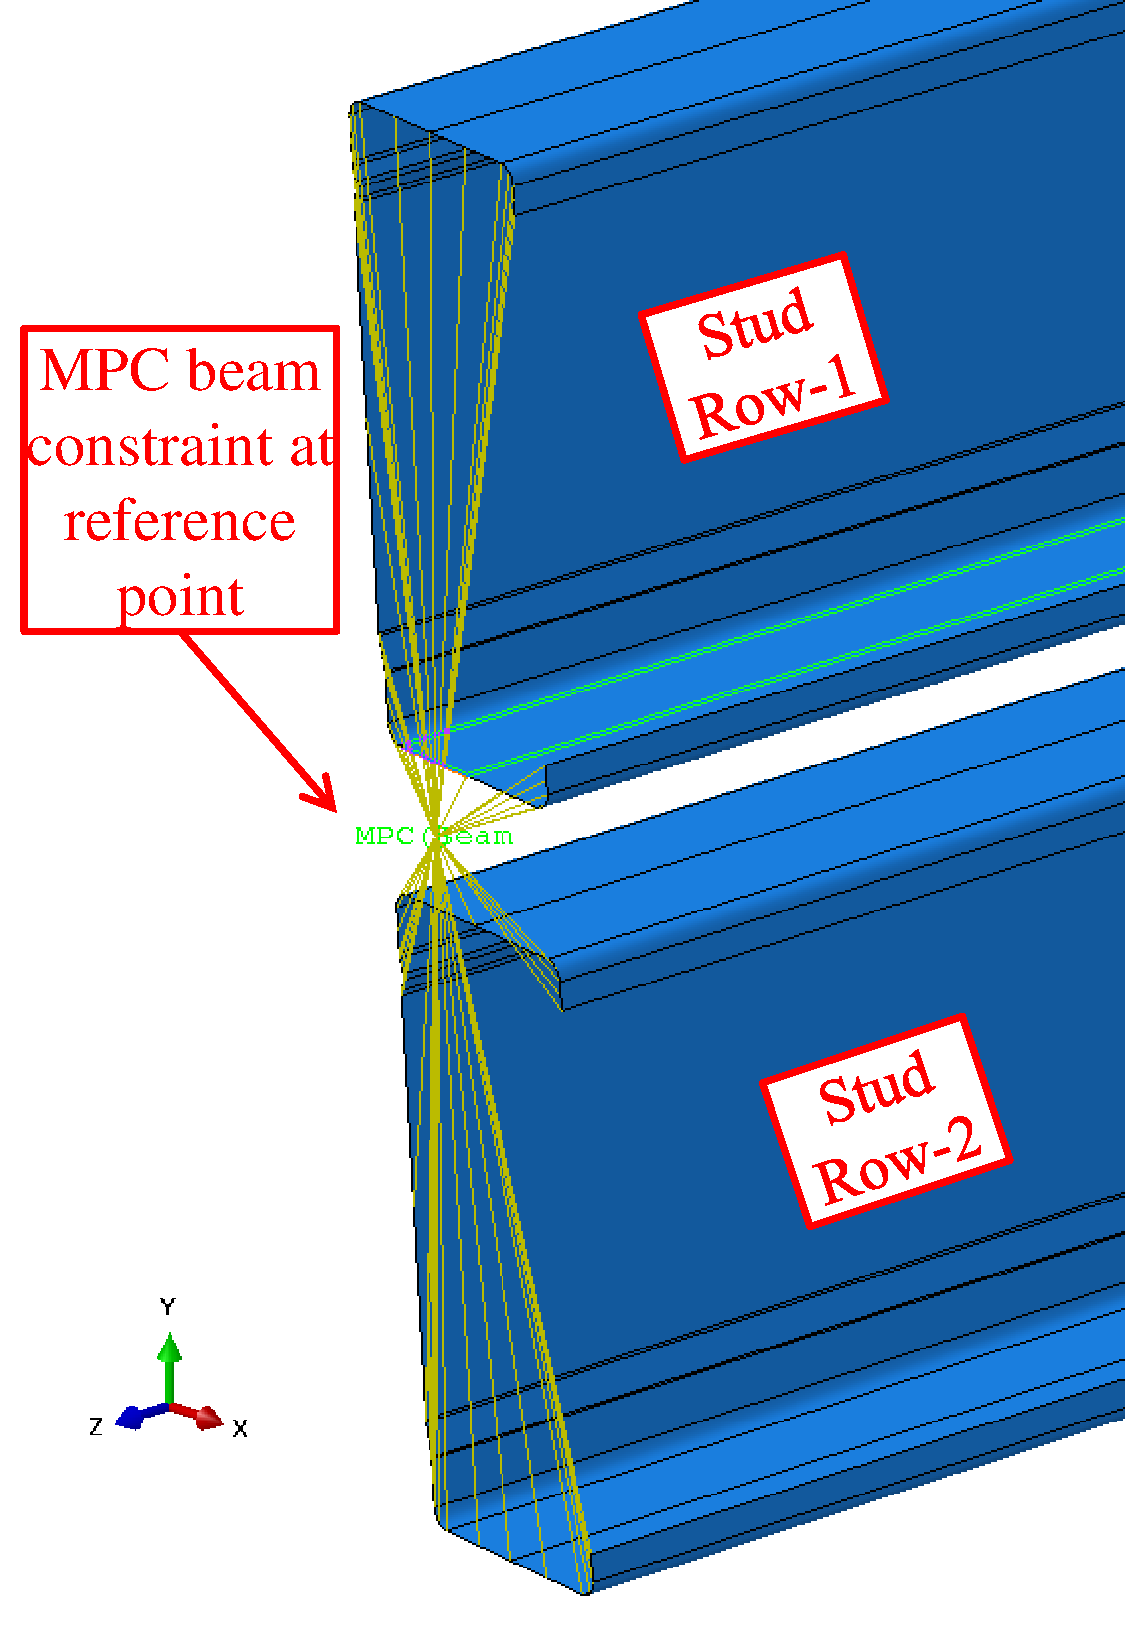
\includegraphics[width=\textwidth]{abaqus-mpc-contraint.pdf}
		\caption{}
		\label{subfig:abaqus-mpc-contraint}
	\end{subfigure}
	\begin{subfigure}[b]{0.4\textwidth}
		\centering
		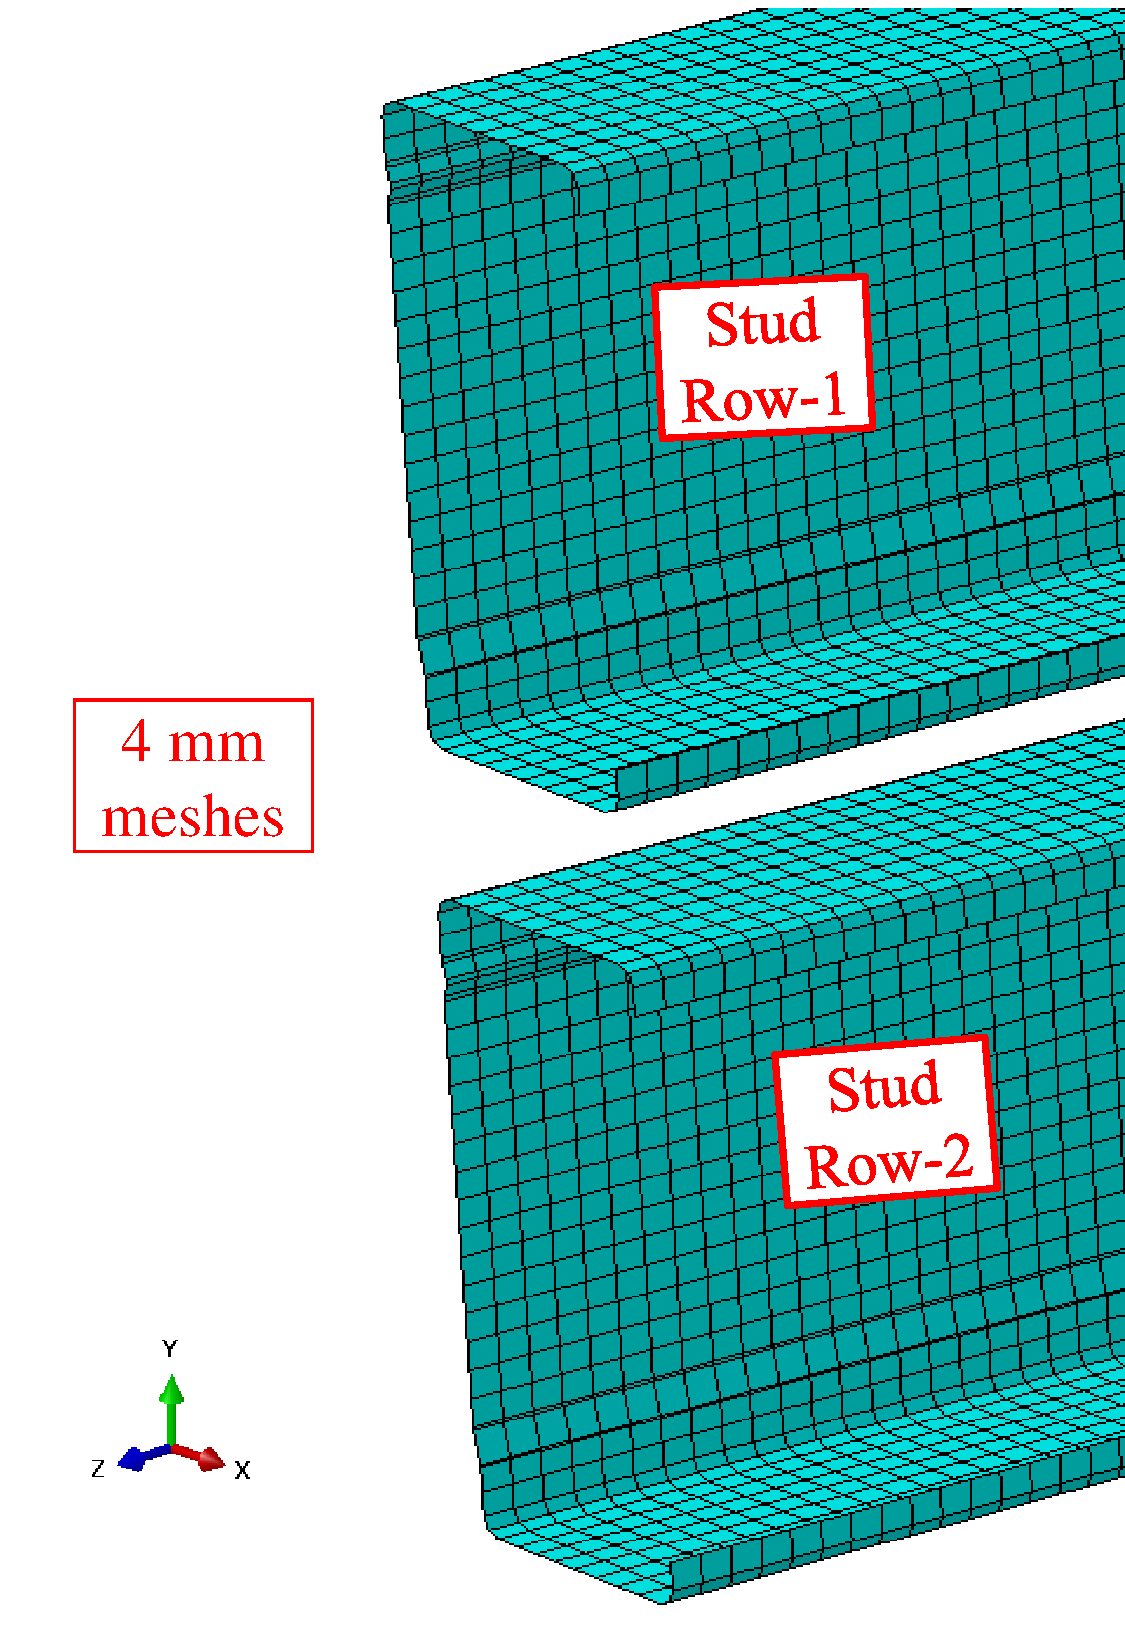
\includegraphics[width=\textwidth]{abaqus-meshes-structural.pdf}
		\caption{}
		\label{subfig:abaqus-meshes-structural}
	\end{subfigure}
	   \caption{Typical double stud model in ABAQUS (a) Support condition (b) Mesh density}
	   \label{fig:abaqus-typical-model}
\end{figure}
\begin{figure}[!htbp]
	\centering
			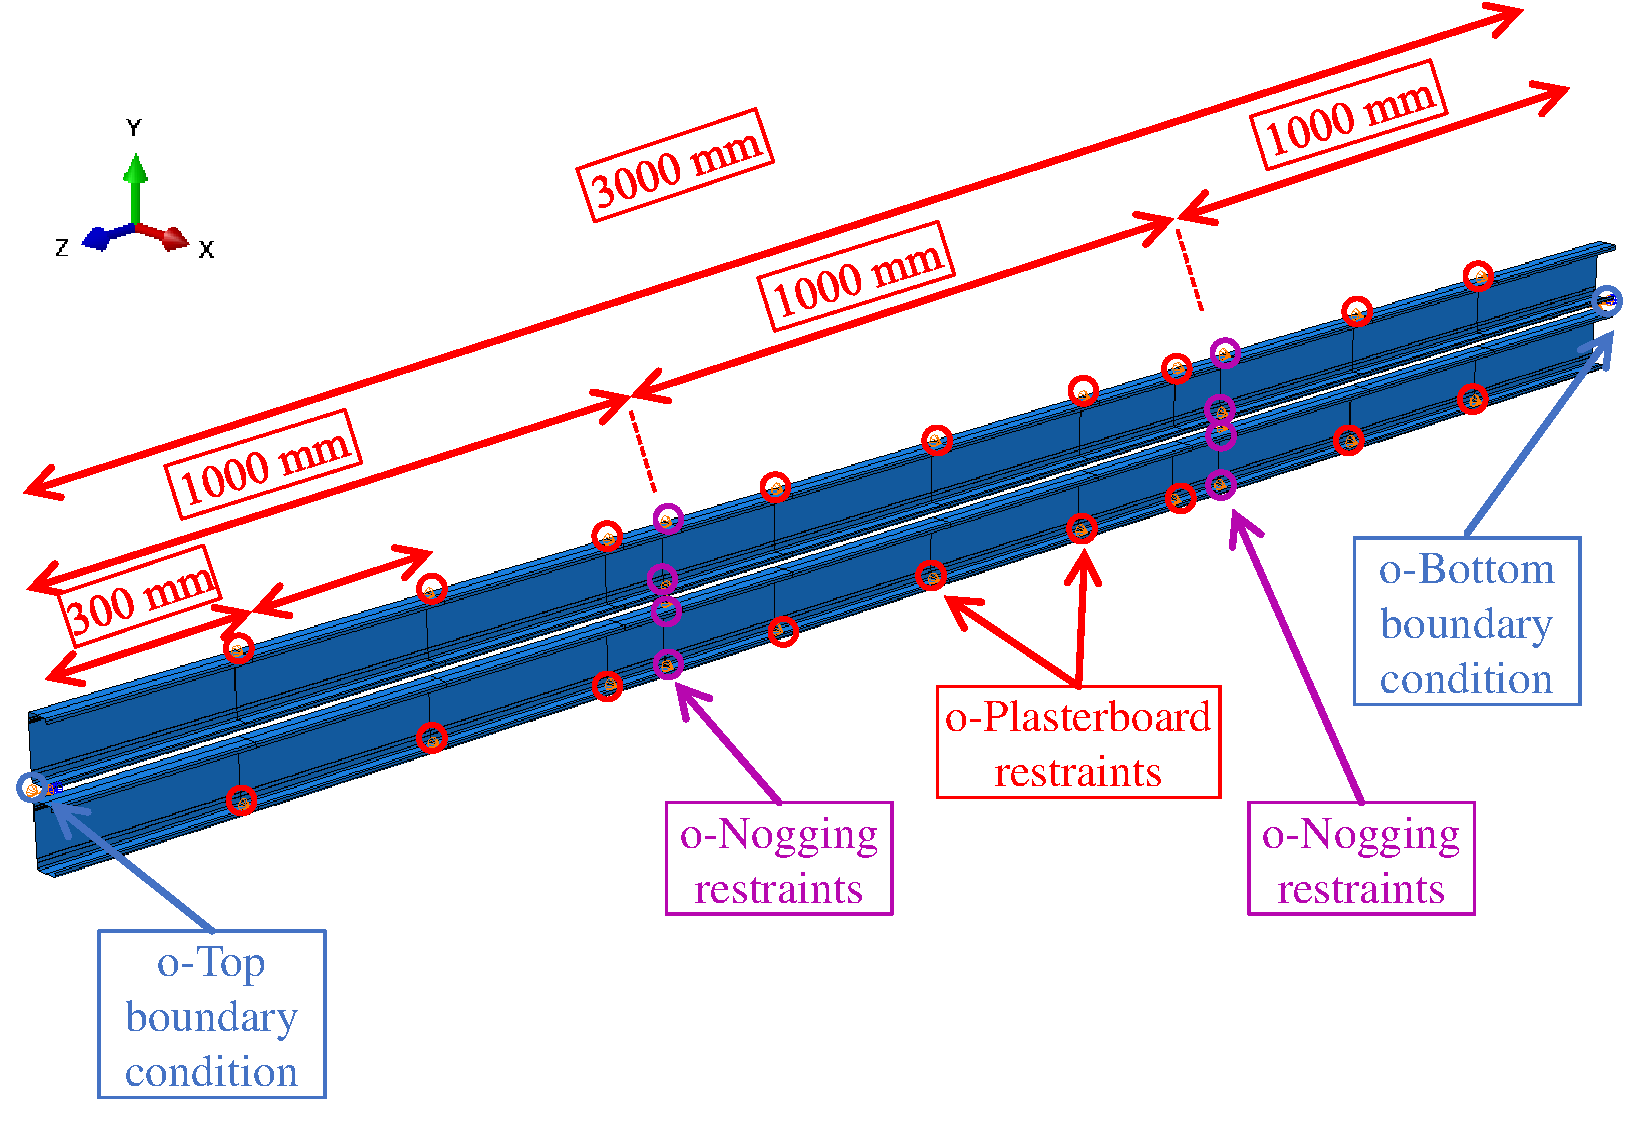
\includegraphics[scale=0.5]{abaqus-assembly-structural.pdf}\\
		\caption{Support and restraint conditions of double stud wall model in ABAQUS}
		\label{fig:abaqus-full-assembly}
\end{figure}

The second step was to conduct non-linear structural analysis and to determine the ultimate load carrying capacity of the studs. The model used for the buckling analysis was imported to a new file to conduct the analysis. The analysis step option was replaced with static general option and the ``Nlgeom" feature was turned on to include the nonlinear effects as a result of large deformation in the model. Maximum increments needed for the analysis are specified depending on the model and also the initial, minimum and maximum increment size. Specific dissipated energy fraction was used for automatic stabilization in the model for better convergence. History output requests were specified at the top reference point to monitor the axial displacement and at the bottom reference point to monitor the support reactions throughout the analysis. These history outputs are stored in the output database (ODB) file for every n\(^{th}\) increment in the analysis. Maximum principal stresses in all the elements throughout the model were also extracted from the analysis. Structural model validation and comparison with the experimental results are discussed next.

\section{Structural FE Model Prediction - Ambient Temperature Capacity Tests}

Structural FE models were developed for all the tested LSF wall configurations listed in \Cref{ch:Ambient}. This includes wall configurations such as single and double stud LSF walls. The load versus axial displacement results from the developed structural FE models are presented and compared with the experimental results next.  

\subsection*{Test-AT1}

Test-AT1 was conducted on a double stud LSF wall with 90 $\times$ 0.95 mm lipped channel studs as shown in \Cref{fig:AT1-plan-fea}. The applied axial compression load versus axial displacement results from finite element analysis (FEA) and experiments are shown in \Cref{fig:AT1-fea-results}. Finite element analysis of Test-AT1 wall resulted a maximum axial compression capacity of 71.97 kN while it was 73.0 kN from the experimental results, a good agreement. However, the gradients of the axial load versus displacement curves from structural FE analysis and experiment do not match well. This is because of the difference in the plasterboard lateral restraint and the end restraint conditions between FE model and experiment. The MPC beam restraint constraints to simulate end supports and the intermittent lateral restraint provided as boundary conditions in the FE model contributes to the difference in slope of the applied load versus axial displacement curve. Modelling the stud to track and stud to plasterboard connection with the appropriate lateral lateral stiffness from the screws in the FE model can eliminate this issue. However, this was beyond the scope of this study.   
\begin{figure}[!htbp]
	\centering
			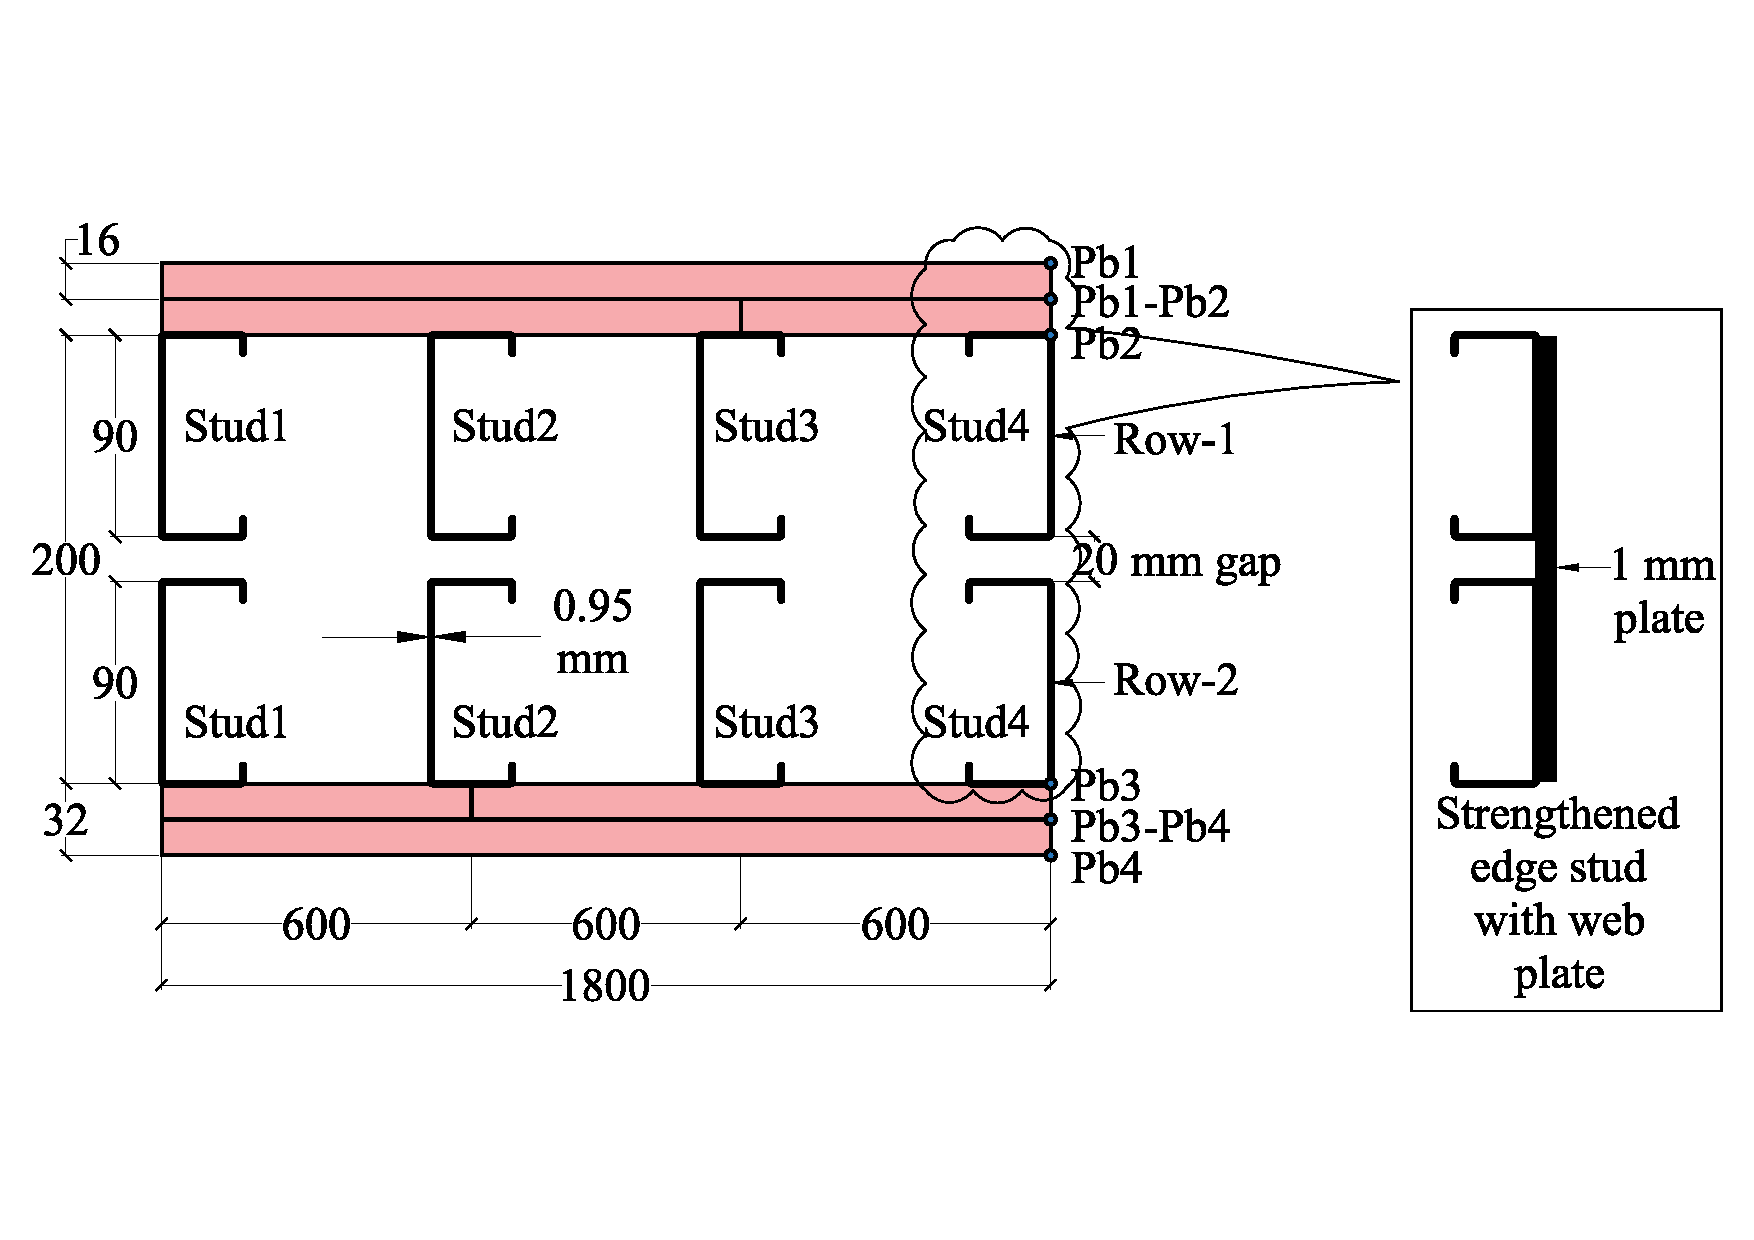
\includegraphics[scale=0.4]{AT1-plan.pdf}\\
		\caption{Test-AT1 wall configuration}
		\label{fig:AT1-plan-fea}
\end{figure}
\begin{figure}[!htbp]
	\centering
			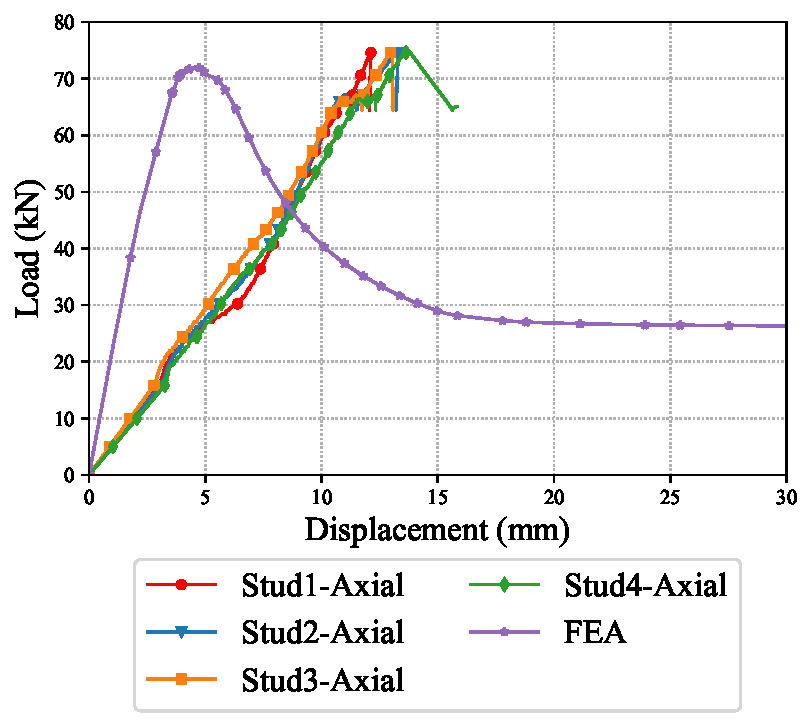
\includegraphics[scale=0.7]{AT1-Load-Axial-Exp-vs-FE.pdf}\\
		\caption{Comparison of load versus displacement curves of Test-AT1 wall from FEA and experiment}
		\label{fig:AT1-fea-results}
\end{figure}
\begin{figure}[!htbp]
	\centering
	\begin{subfigure}[b]{0.4\textwidth}
		\centering
		\includegraphics[width=\textwidth]{AT1-buckling-FEA.pdf}
		\caption{}
		\label{subfig:AT1-buckling-FEA}
	\end{subfigure}
	\begin{subfigure}[b]{0.4\textwidth}
		\centering
		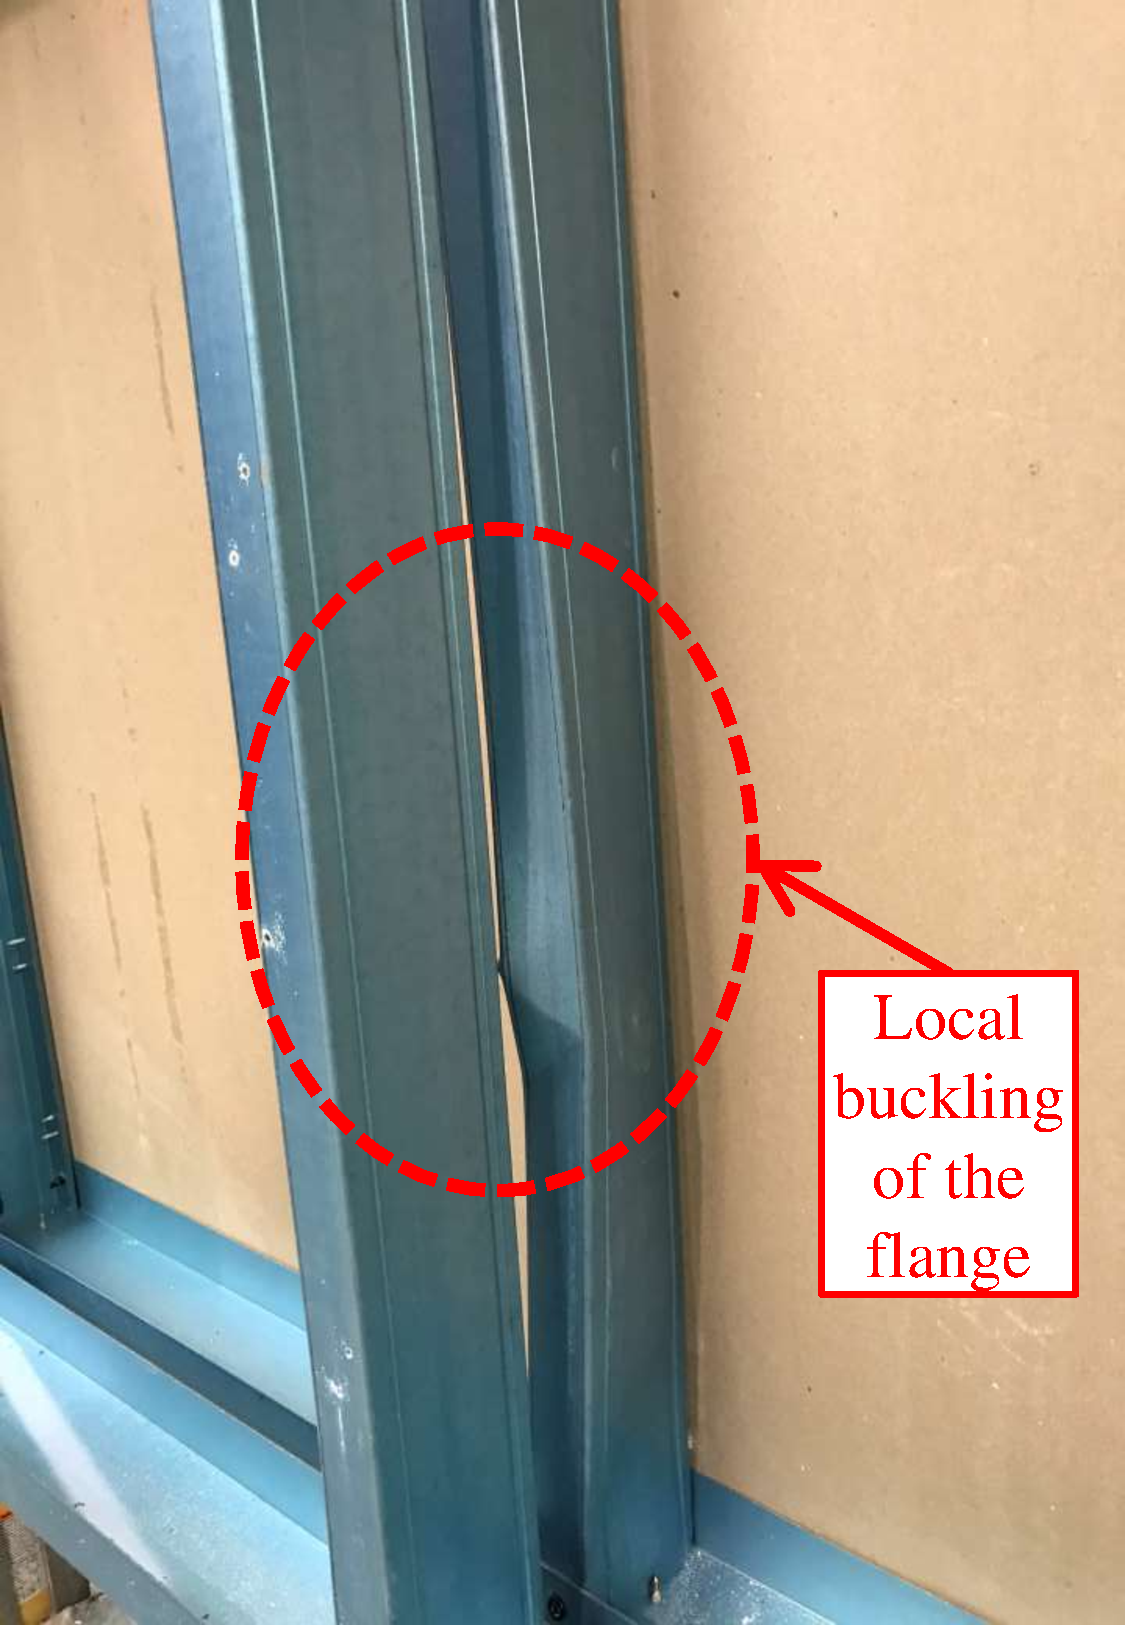
\includegraphics[width=\textwidth]{AT1-buckling.pdf}
		\caption{}
		\label{subfig:AT1-buckling-experiment}
	\end{subfigure}
	   \caption{Buckling failure of studs in Test-AT1 wall (a) FEA (b) Experiment}
	   \label{fig:AT1-buckling-fea-comparison}
\end{figure} 

Since a general static method of analysis was adopted in FEA the axial compression load was applied instantaneously by load control technique in predefined small increments. This might also contribute to the change in the slope of the applied load versus axial displacement curve. The lateral deflections from the FEA are not considered for comparison as local buckling was the dominant mode of failure of studs. The failure mode predicted by FEA is compared with the experimental results in \Cref{fig:AT1-buckling-fea-comparison}. Buckling of the stud flanges observed in the experiments was also simulated by the developed FE model.

\subsection*{Test-AT2}

Test-AT2 was conducted on a double stud LSF walls with 90 $\times$ 0.75 mm lipped channel studs as shown in \Cref{fig:AT2-plan-fea}. The structural FE model gave an axial compression capacity of 46.25 kN while the experimental axial compression capacity was 47.08 kN as shown in \Cref{fig:AT2-fea-results}, a good agreement. The local compressive failure of the stud web and flanges shown in \Cref{subfig:AT2-buckling-FEA} was well simulated by the developed FE model as shown in \Cref{subfig:AT2-buckling-FEA}. It is to be noted that the buckling was significant on one flange of the stud in test wall. However, the stud buckling mode simulation from the FE structural model resulted in the buckling of the flanges and web. This is attributed to the post-ultimate failure behaviour experienced by the stud in the FE model. During the full-scale ambient capacity test after the test wall (first stud) failure, the applied load is transferred to the other studs. As, the edge studs were strengthened the test wall could withstand this excess load for a short time within which the load application was stopped. Therefore, depending upon the time taken to stop the load application after test wall failure is attributed to the post-failure behaviour of the studs in the ambient temperature capacity tests. Also, the stabilization criterion used for Test-T2 was capable of predicting the post-buckling failure. However, determining these factors are based on a trial and error method and varies with the models as stated in the ABAQUS documentation manual (\cite{abaqus2017}).   
\begin{figure}[!htbp]
	\centering
			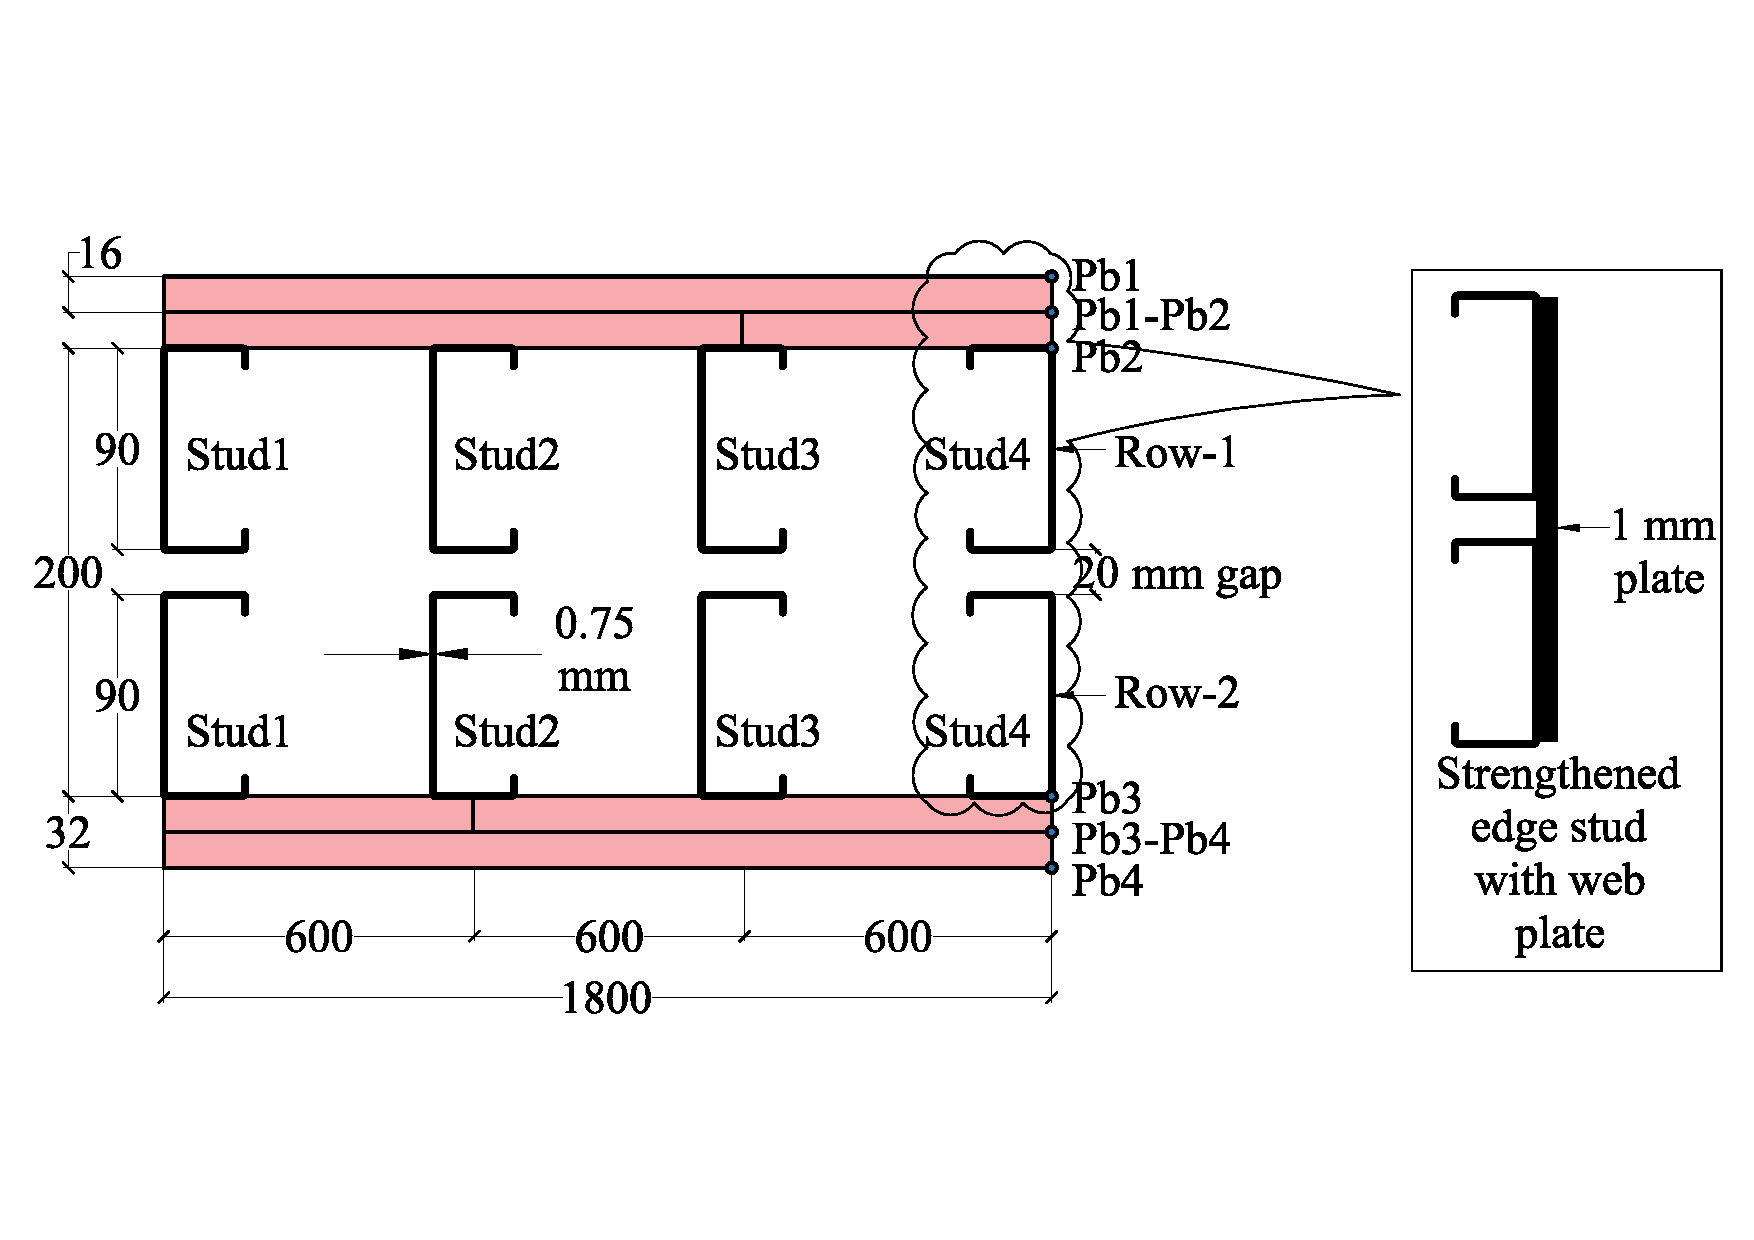
\includegraphics[scale=0.4]{AT2-plan.pdf}\\
		\caption{Test-AT2 wall configuration}
		\label{fig:AT2-plan-fea}
\end{figure}
\begin{figure}[!htbp]
	\centering
			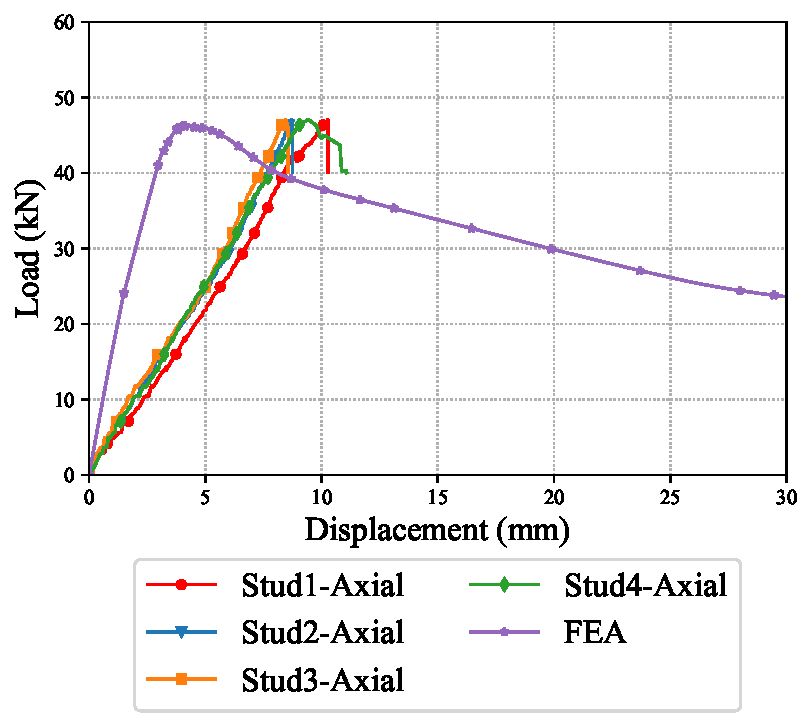
\includegraphics[scale=0.6]{AT2-Load-Axial-Exp-vs-FE.pdf}\\
		\caption{Comparison of load versus displacement curves of Test-AT2 wall from FEA and experiment}
		\label{fig:AT2-fea-results}
\end{figure}
\begin{figure}[!htbp]
	\centering
	\begin{subfigure}[b]{0.4\textwidth}
		\centering
		\includegraphics[width=\textwidth]{AT2-buckling-FEA.pdf}
		\caption{}
		\label{subfig:AT2-buckling-FEA}
	\end{subfigure}
	\begin{subfigure}[b]{0.4\textwidth}
		\centering
		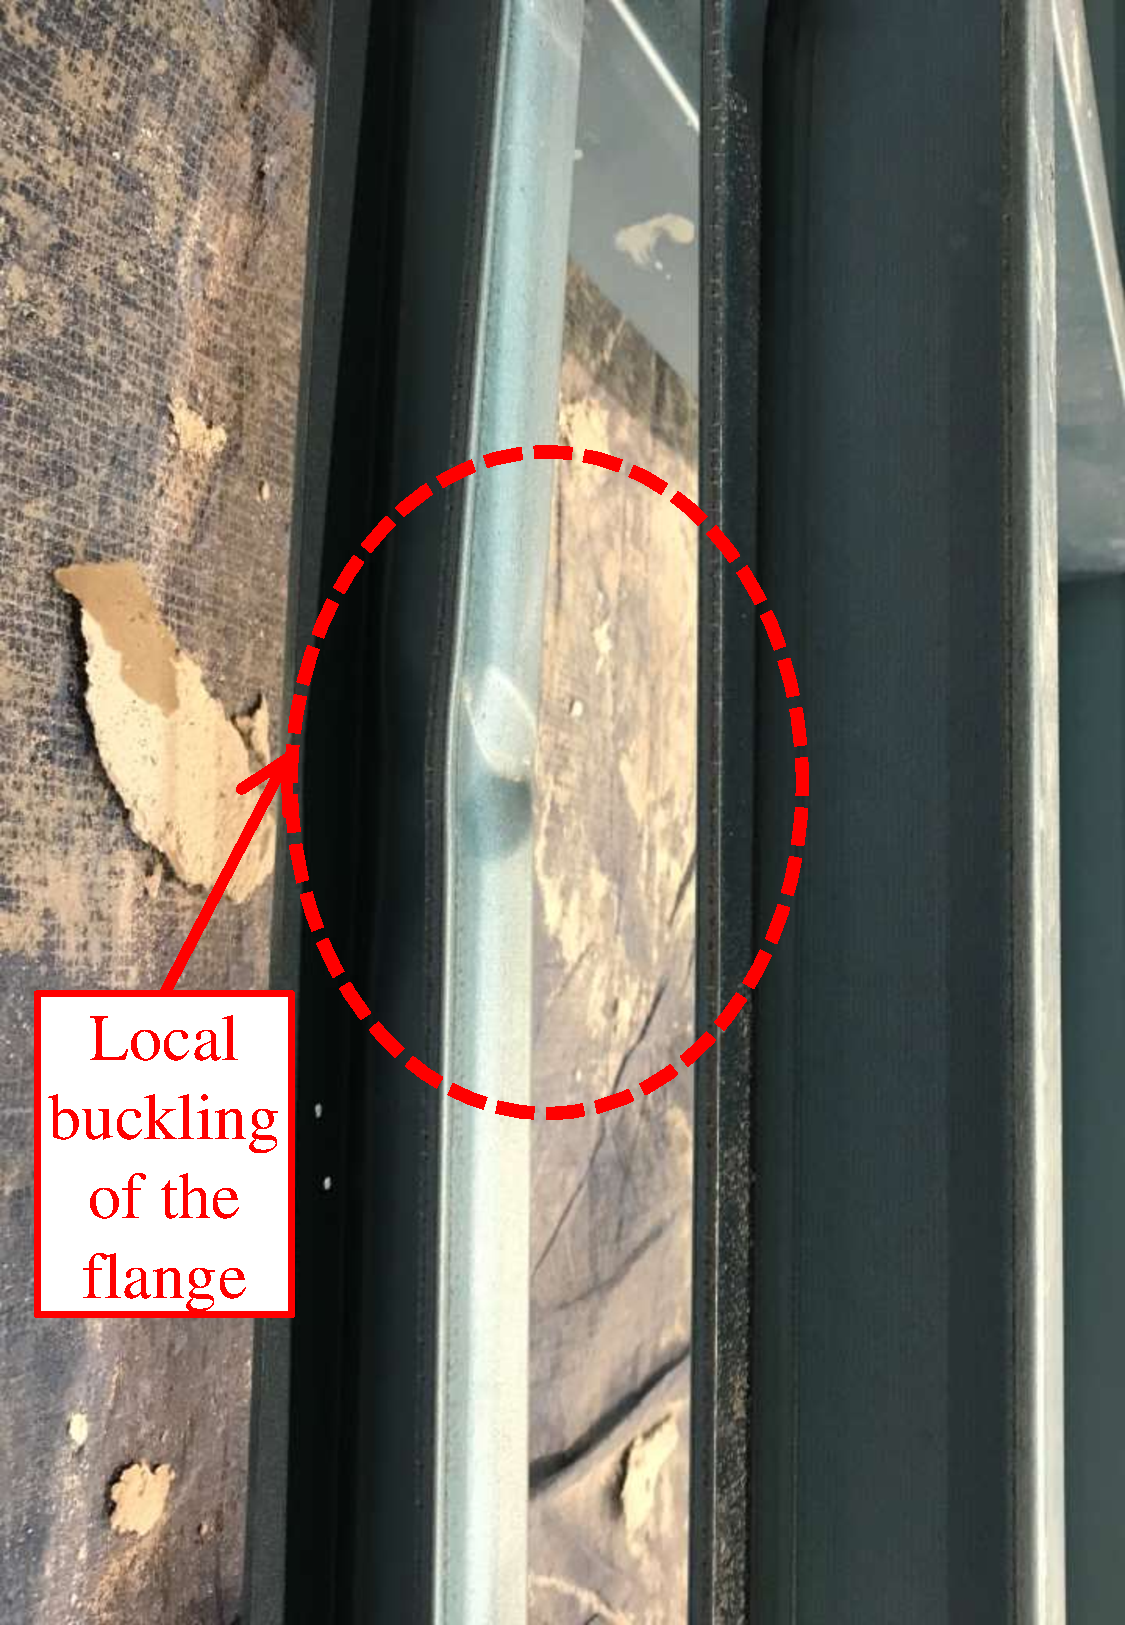
\includegraphics[width=\textwidth]{AT2-buckling.pdf}
		\caption{}
		\label{subfig:AT2-buckling-experiment}
	\end{subfigure}
	   \caption{Buckling failure of studs in Test-AT2 wall (a) FEA (b) Experiment}
	   \label{fig:AT2-buckling-fea-comparison}
\end{figure} 

The ambient temperature tests were conducted on LSF walls with either four or six studs. However, in the developed structural FE models single stud was used for computational efficiency. As discussed in \Cref{sec:AT3} of \Cref{ch:Ambient}, the screw fastened connection of studs with plasterboards and tracks were not considered in the FE model. However, the nodes at the screw locations were provided with full restraints. This was achieved through MPC beam constraints on the end supports and through boundary conditions to simulate intermittent plasterboard restraint on the stud flanges. This assumption holds good as global buckling in the major axis direction was not the dominant failure mode in the ambient temperature capacity tests of double stud walls.

\subsection*{Test-AT3}

As stated earlier Test-AT3 was conducted with six studs unlike four studs in Test-AT2 as shown in \Cref{fig:AT3-plan-fea}. \Cref{fig:AT3-fea} compares the axial compression load versus axial displacement curves from FEA and experiment. The experiment gave an ambient temperature compression capacity of 39.42 kN while the structural FE models prediction was 46.25 kN. However, as stated earlier in \Cref{sec:AT3} of \Cref{ch:Ambient} the reduction in axial compression capacity from the experiment was attributed to the weak plasterboard minor axis restraints provided to the edge studs (Studs1 and 6). As the test wall failed due to the bearing of the edge studs no further comparisons were made for the Test-AT3 with the FE model.   
\begin{figure}[!htbp]
	\centering
			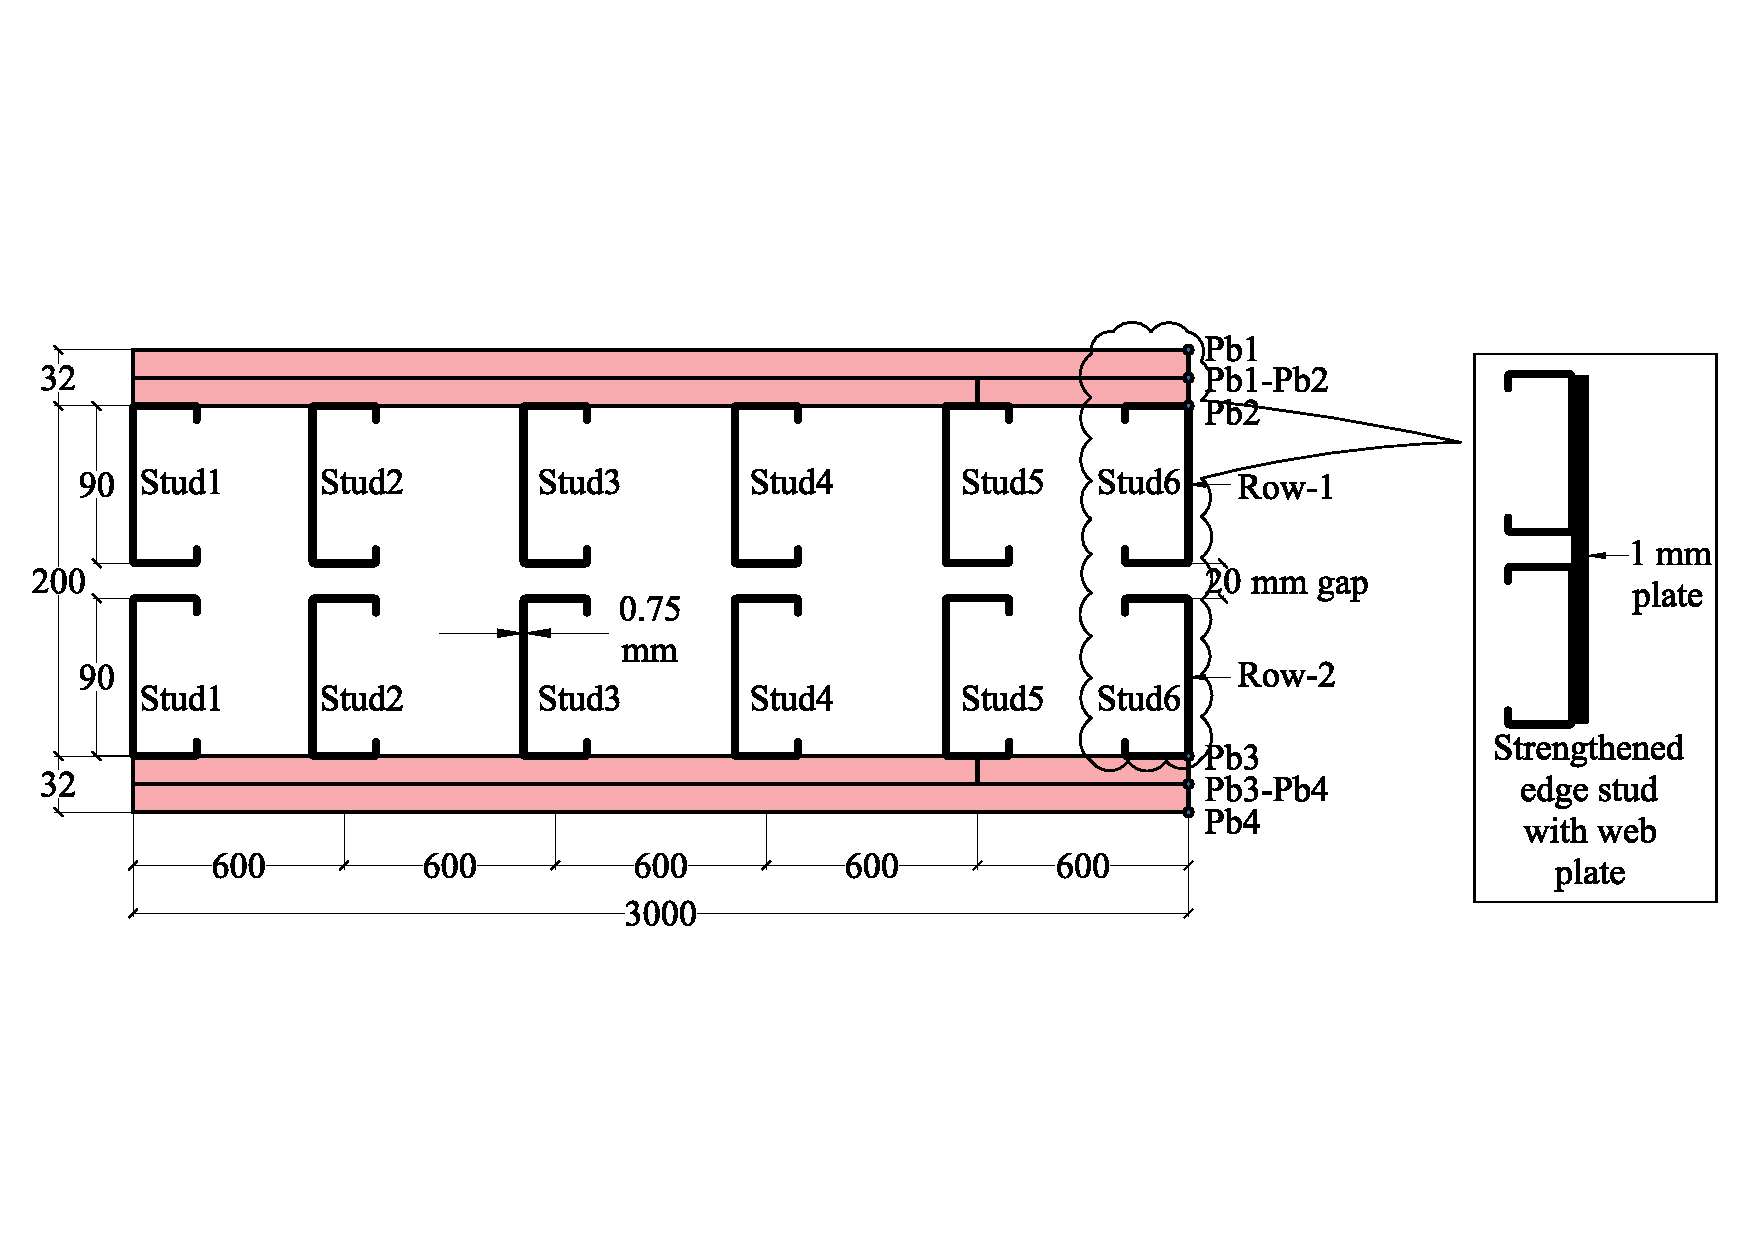
\includegraphics[scale=0.4]{AT3-plan.pdf}\\
		\caption{Test-AT3 wall configuration}
		\label{fig:AT3-plan-fea}
\end{figure}
\begin{figure}[!htbp]
	\centering
			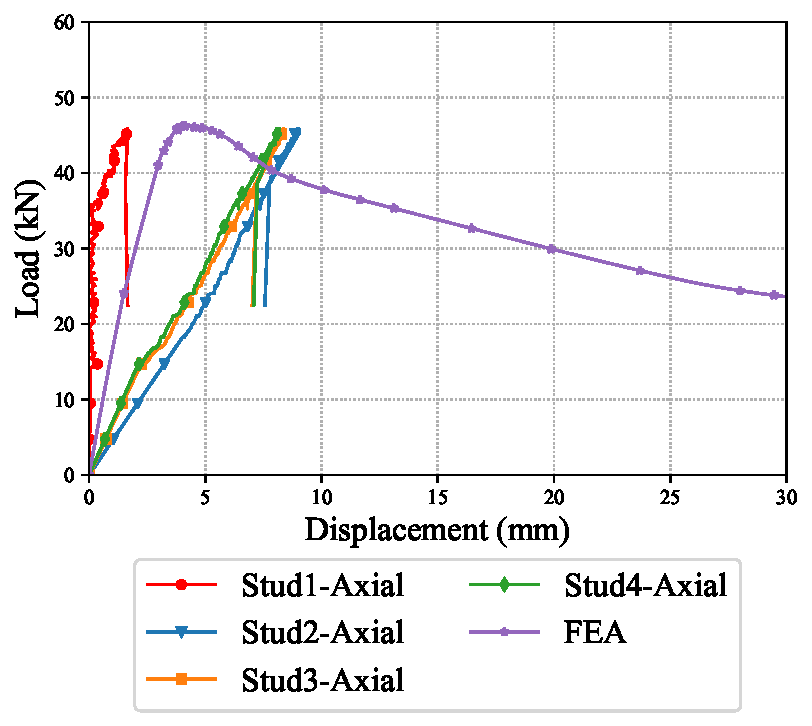
\includegraphics[scale=0.65]{AT3-Load-Axial-Exp-vs-FE.pdf}\\
		\caption{Comparison of load versus displacement curves of Test-AT3 wall from FEA and experiment}
		\label{fig:AT3-fea}
\end{figure}

\subsection*{Test-AT4}

Test-AT4 was conducted on a double stud LSF wall with 70 $\times$ 0.95 mm lipped channel studs as shown in \Cref{fig:AT4-plan-fea}. In this test, the edge studs (Stud1 and 4) were strengthened to avoid premature failures. The structural FE model gave an axial compression capacity of 71.81 kN as shown in \Cref{fig:AT4-fea}. However, the experimental axial compression capacity was 86.21 kN. This higher ambient temperature stud capacity might be due to the higher yield strength of the studs used in the test wall. This was possible because the steel studs for Test-AT4 were procured from a different batch of studs. However, the yield strength used in the structural FE model was the same. Another reason for the higher axial compression capacity from the experiment may be because of the load sharing by the strengthened edge studs. This could have also influenced the applied load versus axial displacement curve exhibiting an intermittent slope as shown in \Cref{fig:AT4-fea}. The buckling of web and flanges observed in the studs in the experiment was simulated well by the developed structural FE model as shown in \Cref{fig:AT4-buckling-fea-comparison}.
\begin{figure}[!htbp]
	\centering
			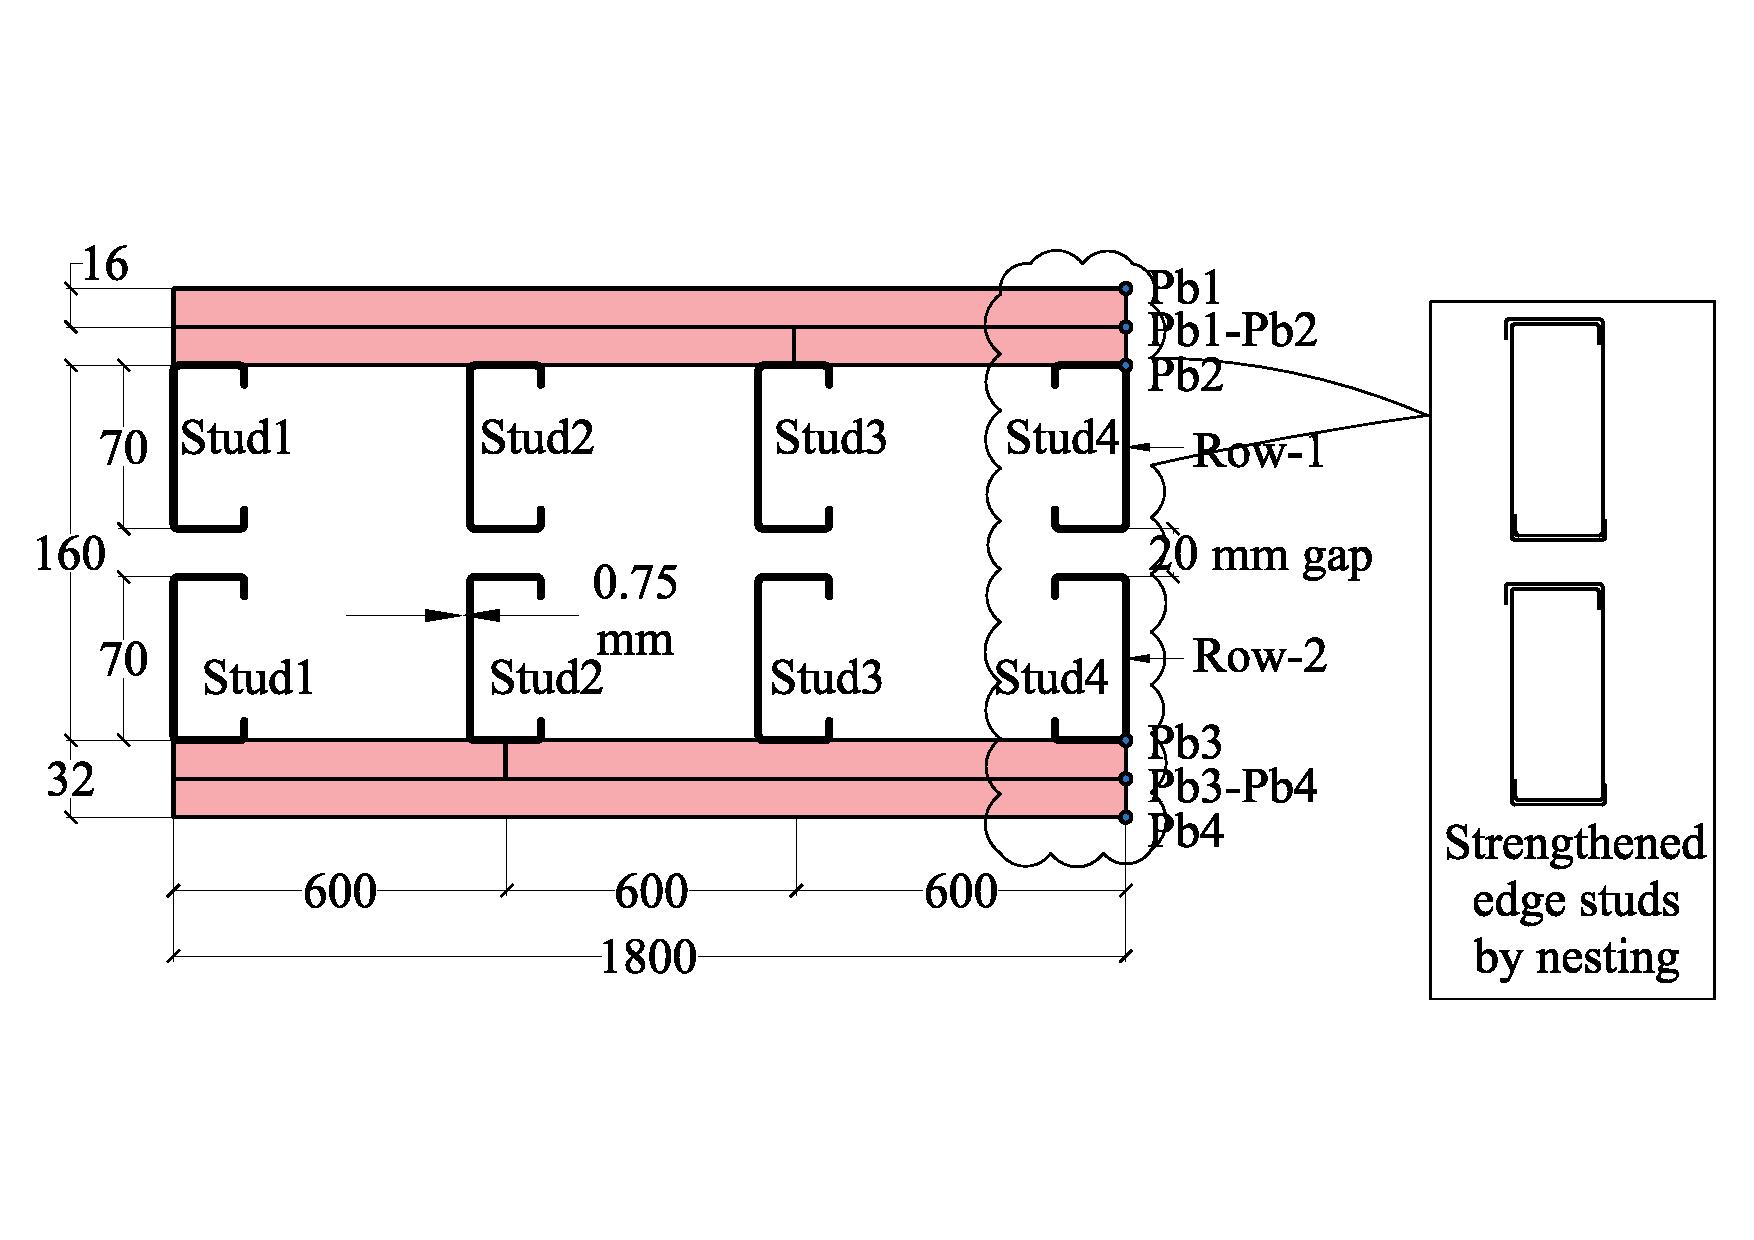
\includegraphics[scale=0.4]{AT4-plan.pdf}\\
		\caption{Test-AT4 wall configuration}
		\label{fig:AT4-plan-fea}
\end{figure}
\begin{figure}[!htbp]
	\centering
			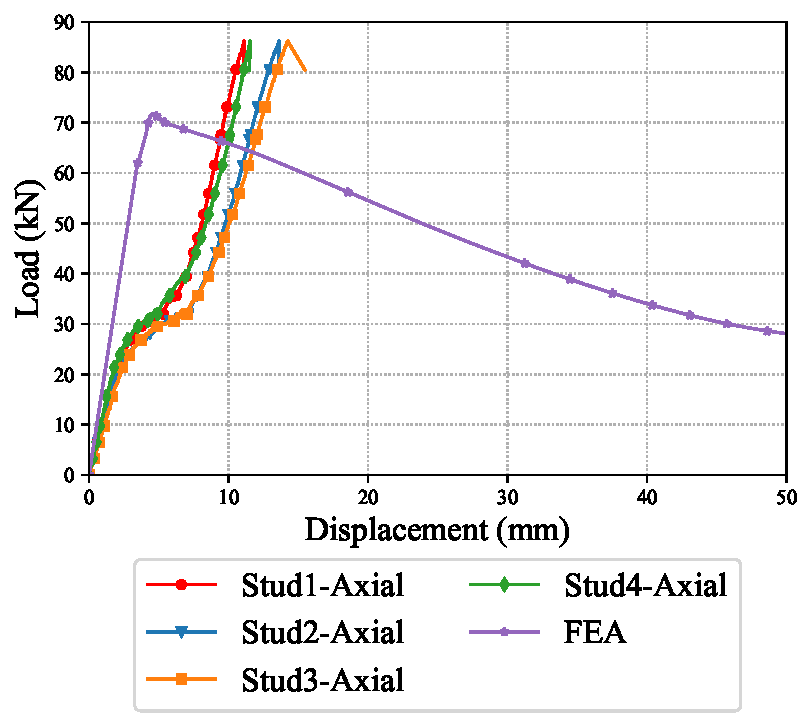
\includegraphics[scale=0.6]{AT4-Load-Axial-Exp-vs-FE.pdf}\\
		\caption{Comparison of load versus displacement curves of Test-AT4 wall from FEA and experiment}
		\label{fig:AT4-fea}
\end{figure}
\begin{figure}[!htbp]
	\centering
	\begin{subfigure}[b]{0.35\textwidth}
		\centering
		\includegraphics[width=\textwidth]{AT4-buckling-FEA.pdf}
		\caption{}
		\label{subfig:AT4-buckling-FEA}
	\end{subfigure}
	\begin{subfigure}[b]{0.35\textwidth}
		\centering
		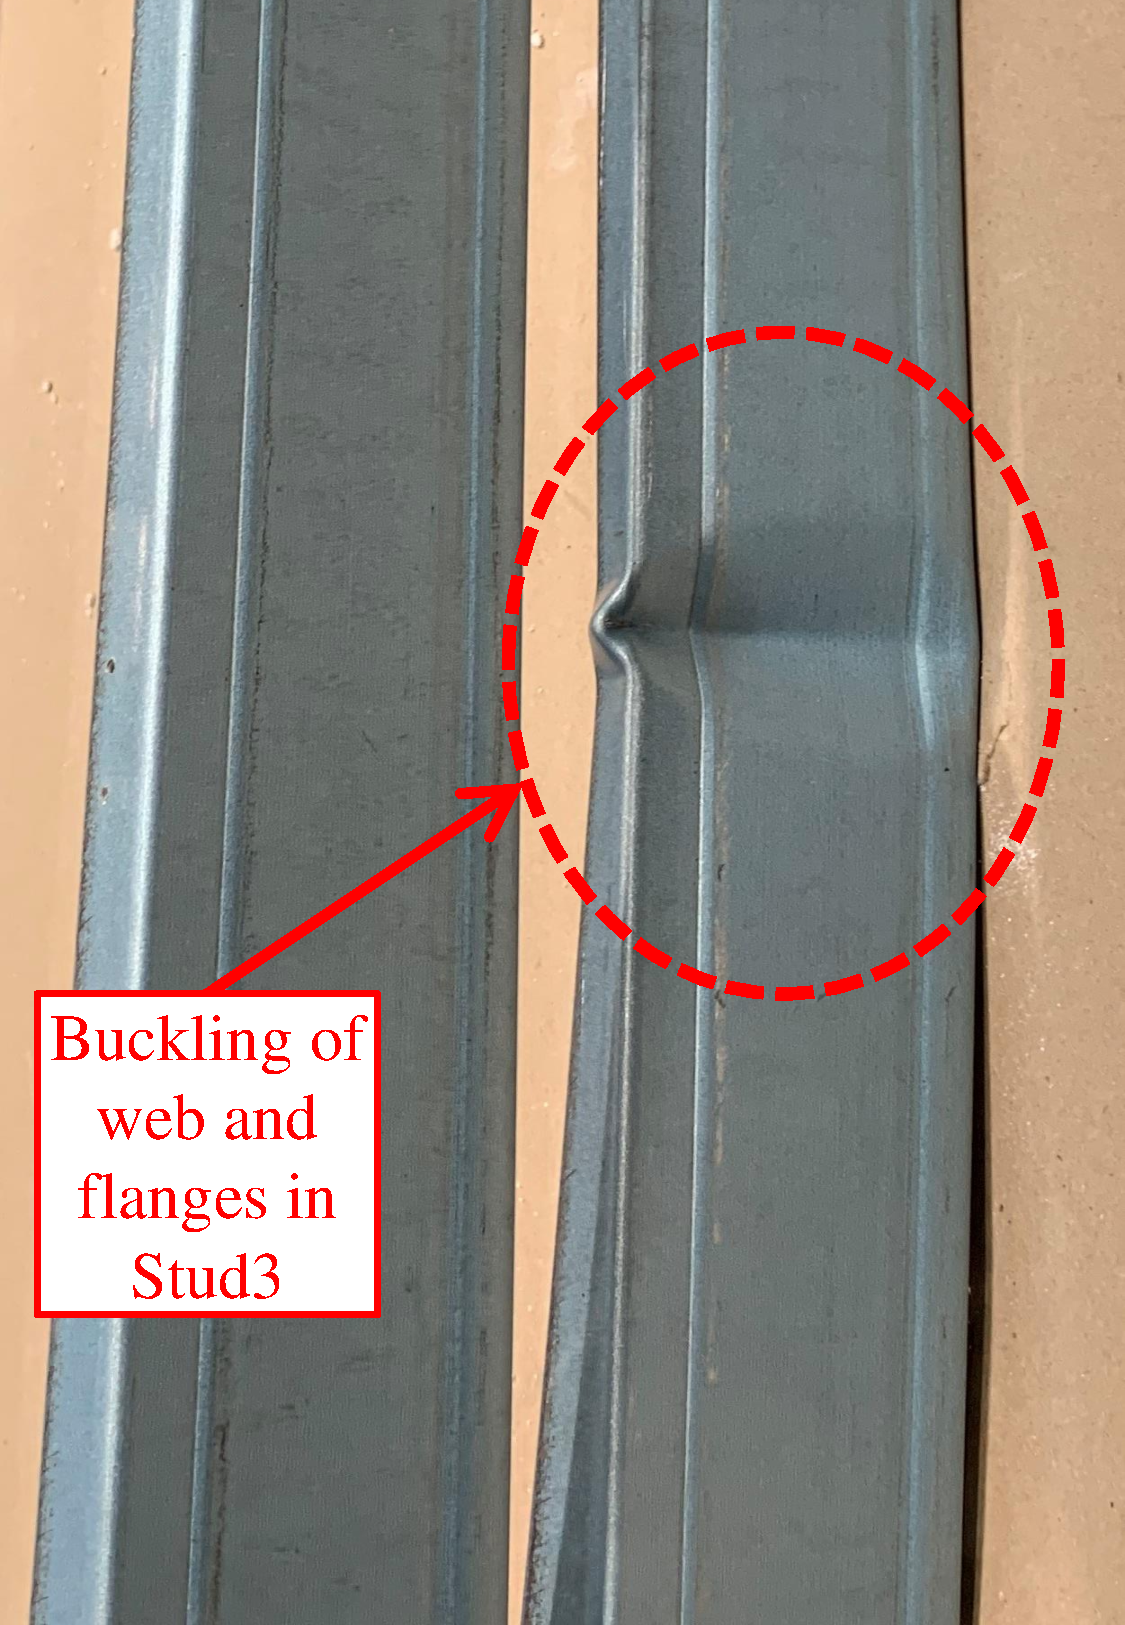
\includegraphics[width=\textwidth]{AT4-buckling.pdf}
		\caption{}
		\label{subfig:AT4-buckling-experiment}
	\end{subfigure}
	   \caption{Buckling failure of studs in Test-AT4 wall (a) FEA (b) Experiment}
	   \label{fig:AT4-buckling-fea-comparison}
\end{figure} 

Local buckling of the web was noticeable in Stud3 Row-1 from the experiment while local buckling was observed in both studs from the FE simulation. This is as a result of post-ultimate failure response simulated by the FE model. The snapshot of the local buckling in the FE model was captured in the last time step of the simulation corresponding to the axial displacement of 40 mm from load versus displacement curve shown in \Cref{fig:AT4-fea}. 
 
\subsection*{Test-AT5}

Test-AT5 was conducted on a staggered stud LSF wall made of 90 $\times$ 0.95 mm lipped channel studs as shown in \Cref{fig:AT5-plan-fea}. The modelling technique adapted to simulate the ambient capacity Test-AT5 was different in comparison with the other four ambient capacity tests. This is because of the use of omega noggings in the experimental set-up. As the noggings were connected through the webs instead of flanges in the experimental test wall, similar set-up was adapted in the structural FE model. Firstly, service holes were made on the studs at 1 m interval. The studs were arranged at 300 mm apart in the ASSEMBLY. A Reference Point (RP) was created at the top and bottom centroid of the wall system as shown in \Cref{subfig:AT5-mpc-constraint-top}. Top and bottom boundary conditions along with the axial load were applied through these RPs. Partitions were created around the service holes to facilitate the application of MPC beam constraints. This was done by selecting the edges of the service holes as the slave edges connecting to a master node at the centre of service hole through MPC beam constraint as shown in \Cref{subfig:AT5-mpc-constraint-nogging}. A RP was created at the centre of all the service holes and the nogging restraints were provided as boundary condition. Translation along the x-axis was fixed at the RP to simulate the minor axis restraint provided by the omega nogging on the stud web. Details about the MPC-constraints on the service holes of the studs are shown in \Cref{subfig:AT5-mpc-constraint-nogging}. Meshing near the stud service holes is critical in the structural FE model. Therefore, partitions were created around the stud service holes in the ASSEMBLY to create a sweep mesh around the service holes as shown in \Cref{subfig:AT5-mesh}. The structural analysis was conducted using a similar procedure to that of Tests-AT1 to AT4 incorporating the above-mentioned changes in the model.
\begin{figure}[!htbp]
	\centering
			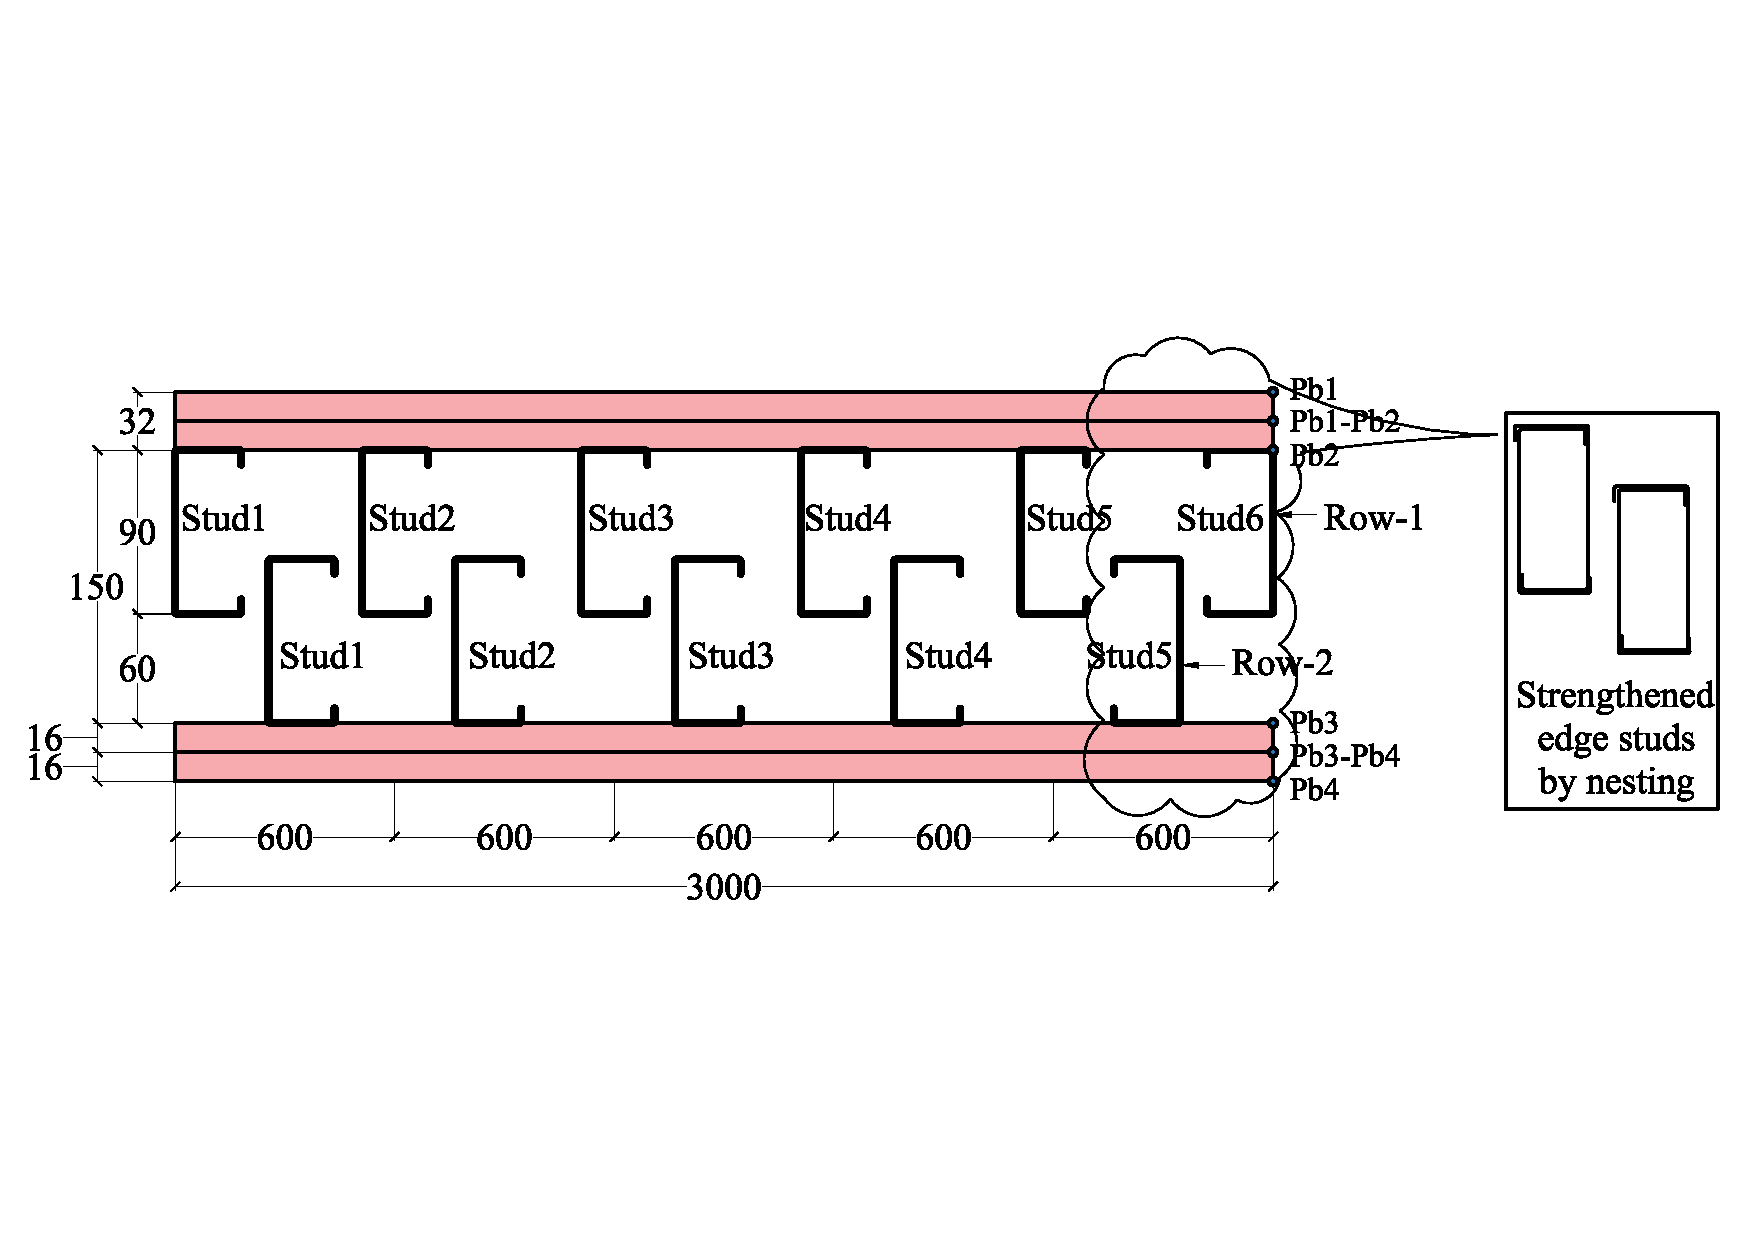
\includegraphics[scale=0.4]{AT5-plan.pdf}\\
		\caption{Test-AT5 wall configuration}
		\label{fig:AT5-plan-fea}
\end{figure}    
\begin{figure}[!htbp]
	\centering
	\begin{subfigure}[b]{0.3\textwidth}
		\centering
		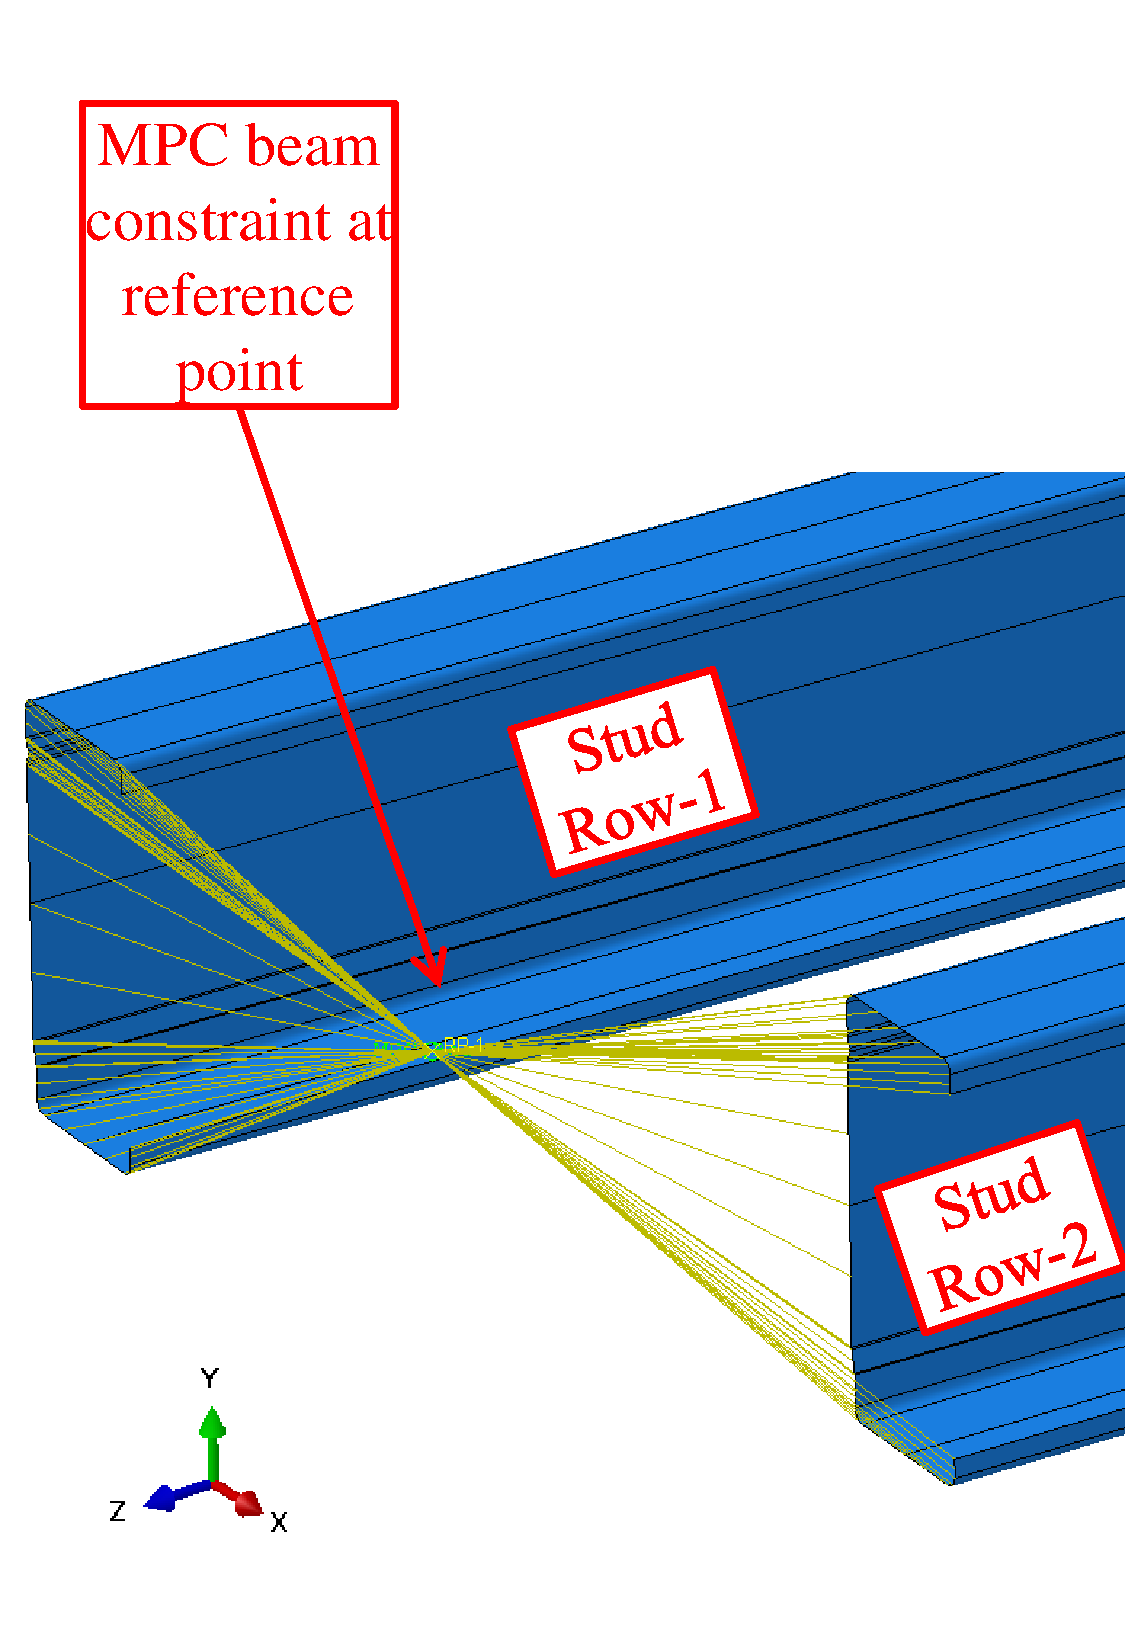
\includegraphics[width=\textwidth]{AT5-mpc-constraint-top.pdf}
		\caption{}
		\label{subfig:AT5-mpc-constraint-top}
	\end{subfigure}
	\begin{subfigure}[b]{0.5\textwidth}
		\centering
		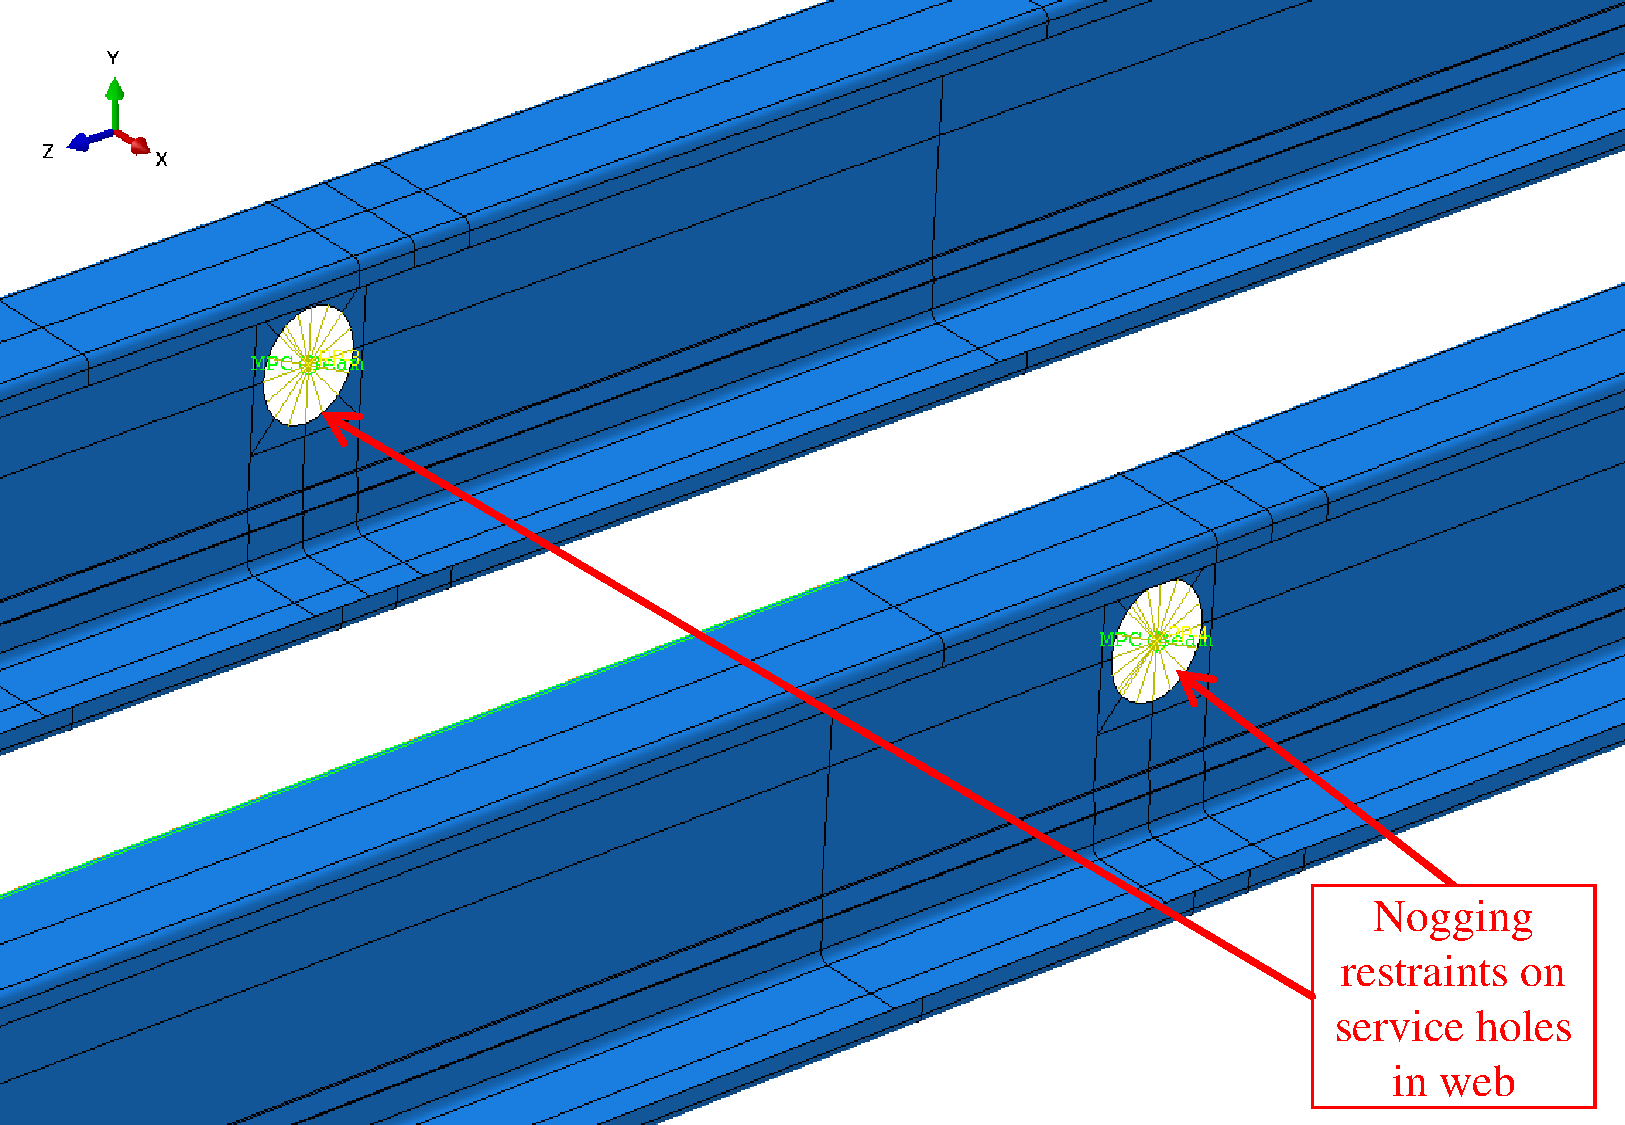
\includegraphics[width=\textwidth]{AT5-mpc-constraint-nogging.pdf}
		\caption{}
		\label{subfig:AT5-mpc-constraint-nogging}
	\end{subfigure}
	\begin{subfigure}[b]{0.5\textwidth}
		\centering
		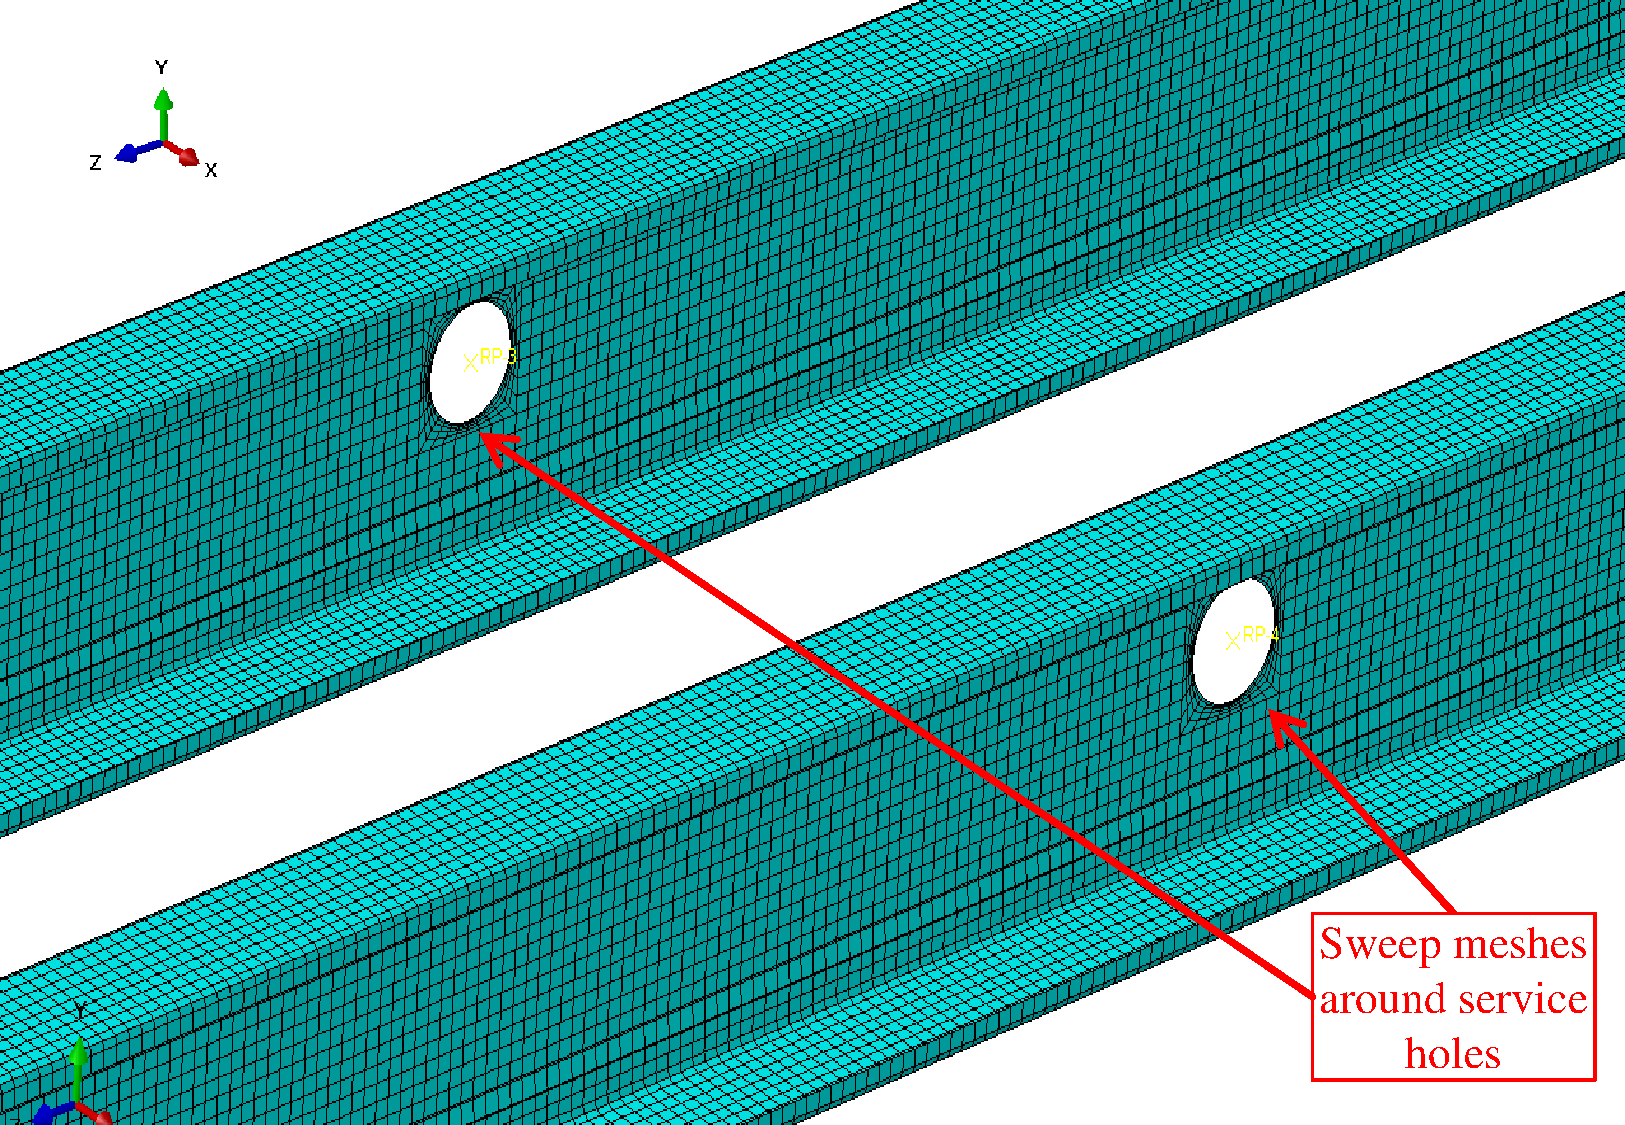
\includegraphics[width=\textwidth]{AT5-mesh.pdf}
		\caption{}
		\label{subfig:AT5-mesh}
	\end{subfigure}
	   \caption{Test-AT5 - Staggered stud model (a) MPC beam constraints to simulate end restraints (b) MPC beam constraints at service holes to simulate nogging restraints (c) Sweep meshes around service holes}
	   \label{fig:AT5-modelling-fea}
\end{figure} 
\begin{figure}[!htbp]
	\centering
		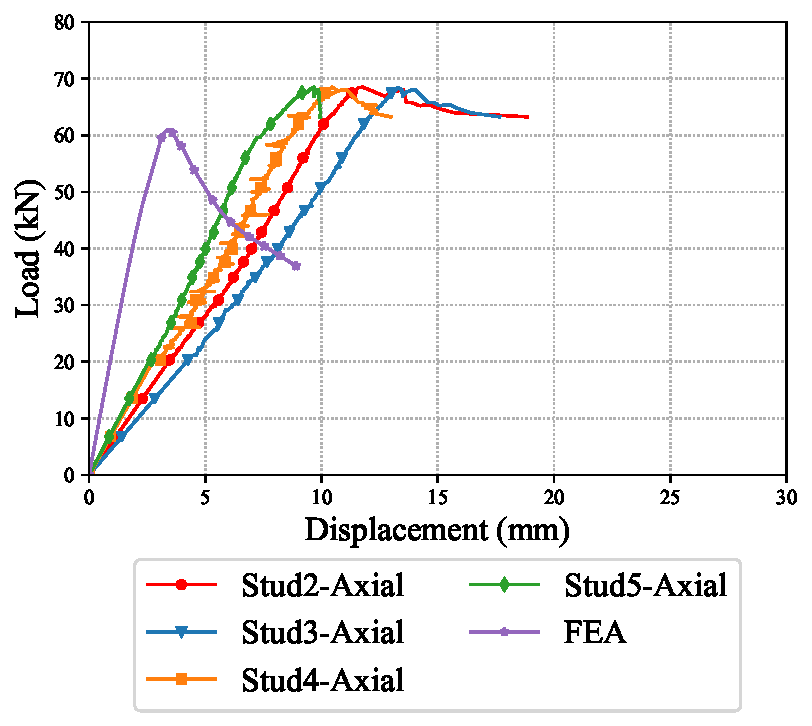
\includegraphics[scale=0.6]{AT5-Load-Axial-Exp-vs-FE.pdf}\\
		\caption{Comparison of load versus displacement curves of Test-AT5 wall from FEA and experiment}
	\label{fig:AT5-fea}
\end{figure}
\begin{figure}[!htbp]
	\centering
	\begin{subfigure}[b]{0.4\textwidth}
		\centering
		\includegraphics[width=\textwidth]{AT5-buckling-FEA.pdf}
		\caption{}
		\label{subfig:AT5-buckling-FEA}
	\end{subfigure}
	\begin{subfigure}[b]{0.4\textwidth}
		\centering
		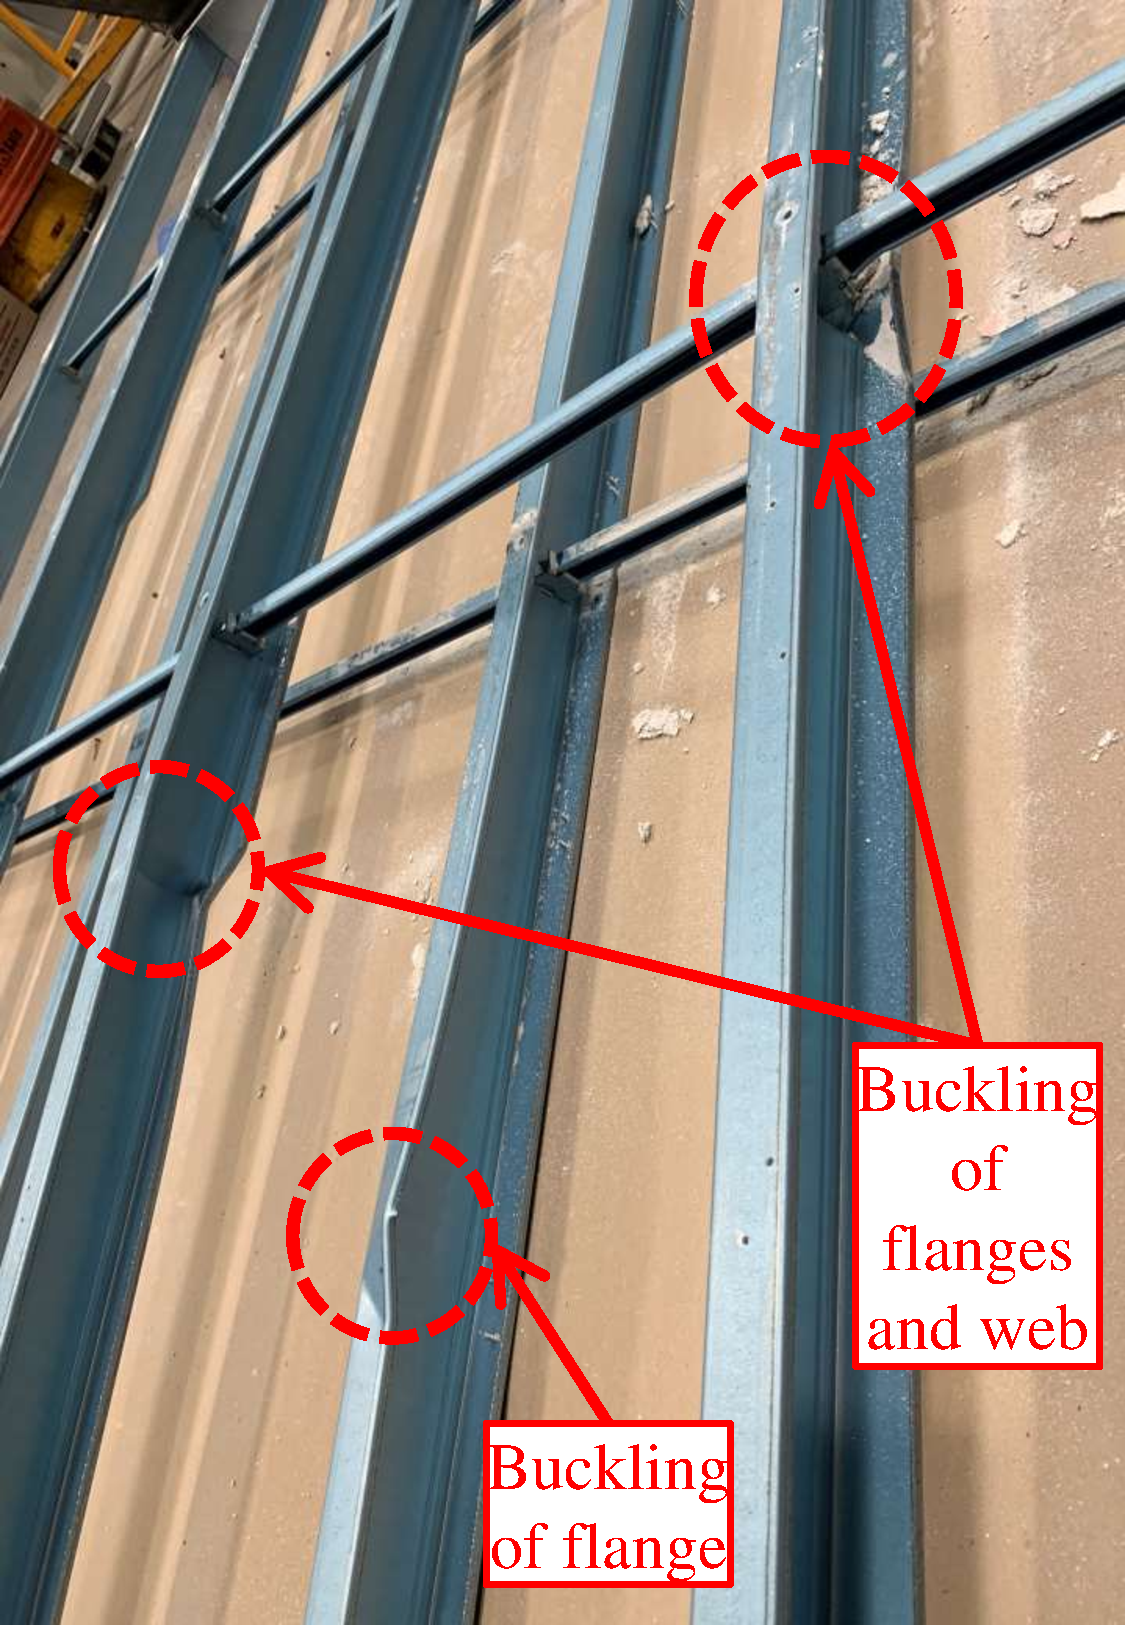
\includegraphics[width=\textwidth]{AT5-buckling.pdf}
		\caption{}
		\label{subfig:AT5-buckling-experiment}
	\end{subfigure}
	   \caption{Buckling failure of studs in Test-AT5 wall (a) FEA (b) Experiment}
	   \label{fig:AT5-buckling-fea-comparison}
\end{figure} 

\Cref{fig:AT5-fea} compares the axial compression load versus axial displacement curves from structural FE model and experiment. The structural FE model gave an axial compression capacity of 60.98 kN in comparison with the experimental capacity of 68.49 kN. Buckling of the stud web and flanges near the service holes observed in the experiment was simulated well by the developed structural FE model as shown in \Cref{fig:AT5-buckling-fea-comparison}. 

\section{Summary of Ambient Temperature Capacity Predictions}

A summary of the ambient temperature capacities predicted by the structural FE model is shown in \Cref{tab:ambient-test-results-fea}. Comparison with experimental capacities show that the developed structural FE model could determine the structural failure capacity of the double and staggered stud LSF walls under ambient temperature conditions to a reasonable accuracy except for Test-AT4 (16.7\% lower prediction). The buckling failure modes corresponding to all the ambient capacity tests were also simulated to a reasonable accuracy in all the ambient temperature capacity models. Therefore, this structural FE model was further extended to include temperature boundary conditions in studs to predict the failure time of these complex LSF walls exposed to fire conditions. 
% Table generated by Excel2LaTeX from sheet 'Sheet5'
\begin{table}[htbp]
	\centering
	\caption{Ambient temperature capacity predictions by FEA and comparison with experimental capacities}
	  \begin{tabular}{ccccc}
	  \toprule
	  \multicolumn{1}{m{3em}}{\multirow{2}{3em}{\centering{Test Name}}} & 
	  \multirow{2}[4]{*}{Description} & 
	  \multicolumn{2}{m{5.075em}}{\centering{Failure capacity (kN)}} & 
	  \multicolumn{1}{m{5em}}{\multirow{2}{4em}{\centering{Ratio of \newline{}FEA/Test capacity}}} \\
  \cmidrule{3-4}          &       & Test  & FEA   &  \\
	  \midrule
	  AT1   & Double Stud - 90 $\times$ 0.95 - 4 studs & 73.00 & 71.97 & -1.03 \\
	  AT2   & Double Stud - 90 $\times$ 0.75 - 4 studs & 47.08 & 46.25 & -0.83 \\
	  AT3   & Double Stud - 90 $\times$ 0.75 - 6 studs & 39.42 & 46.25 & 6.83 \\
	  AT4   & Double Stud - 70 $\times$ 0.95 - 4 studs & 86.21 & 71.81 & -14.40 \\
	  AT5   & Staggered  Stud - 90 $\times$ 0.95 - 11 studs & 68.49 & 60.98 & -7.51 \\
	  \bottomrule
	  \end{tabular}%
	\label{tab:ambient-test-results-fea}%
  \end{table}%
  
\section[Coupled Temperature Displacement Structural Analysis]{Coupled Temperature Displacement \\Structural Analysis}\label{sec:temp-disp-structural}

After determining the ambient temperature capacities in \Cref{ch:Ambient}, the failure times of the tested LSF walls in fire from \Cref{ch:Fire} were considered for investigation. Full-scale fire Tests-T1 to T7 and T10 conducted under load-bearing conditions were considered in the numerical investigation of this chapter. The non-load bearing fire Tests-T8 and T9 were investigated in \Cref{ch:FE-Parametric}. The aim of the coupled temperature displacement structural analysis was to determine the failure times of the tested wall configurations under specified temperature boundary conditions along with axial compression load. 3D shell elements were used in the analysis using S4RT element which supports temperature degree of freedom. Temperatures on the hot and cold flanges were extracted from the FDS thermal models from \Cref{ch:FE-Thermal} and were incorporated as boundary conditions on to the stud hot and cold flanges in the structural model. Attempts were also made to extract the stud hot and cold flange temperatures from Test-T1 wall and the degree of agreement in the failure time between the developed FE model and experiment was investigated. This technique was employed to investigate the credibility of the developed structural FE model using sequentially coupled-temperature displacement analysis. Temperature boundary conditions on the stud webs was assumed to vary linearly based on the hot and cold flange temperatures and applied to the stud nodes along the length as shown in \Cref{fig:temperature-gradient-stud}. Linear temperature variation along the web is governed by the number of mesh nodes on the stud web. However, the fire and ambient side hot and cold flanges had no variations in the input temperature boundary condition. Concentrated force from the initial non-linear structural ambient temperature analysis was applied at the reference point on the top of the FE model. This assumption was based on \citet{Ariyanayagam2018b} to model the structural response of single stud LSF walls in fire. A similar approach was followed in this investigation as well.  
\begin{figure}[!htbp]
	\centering
			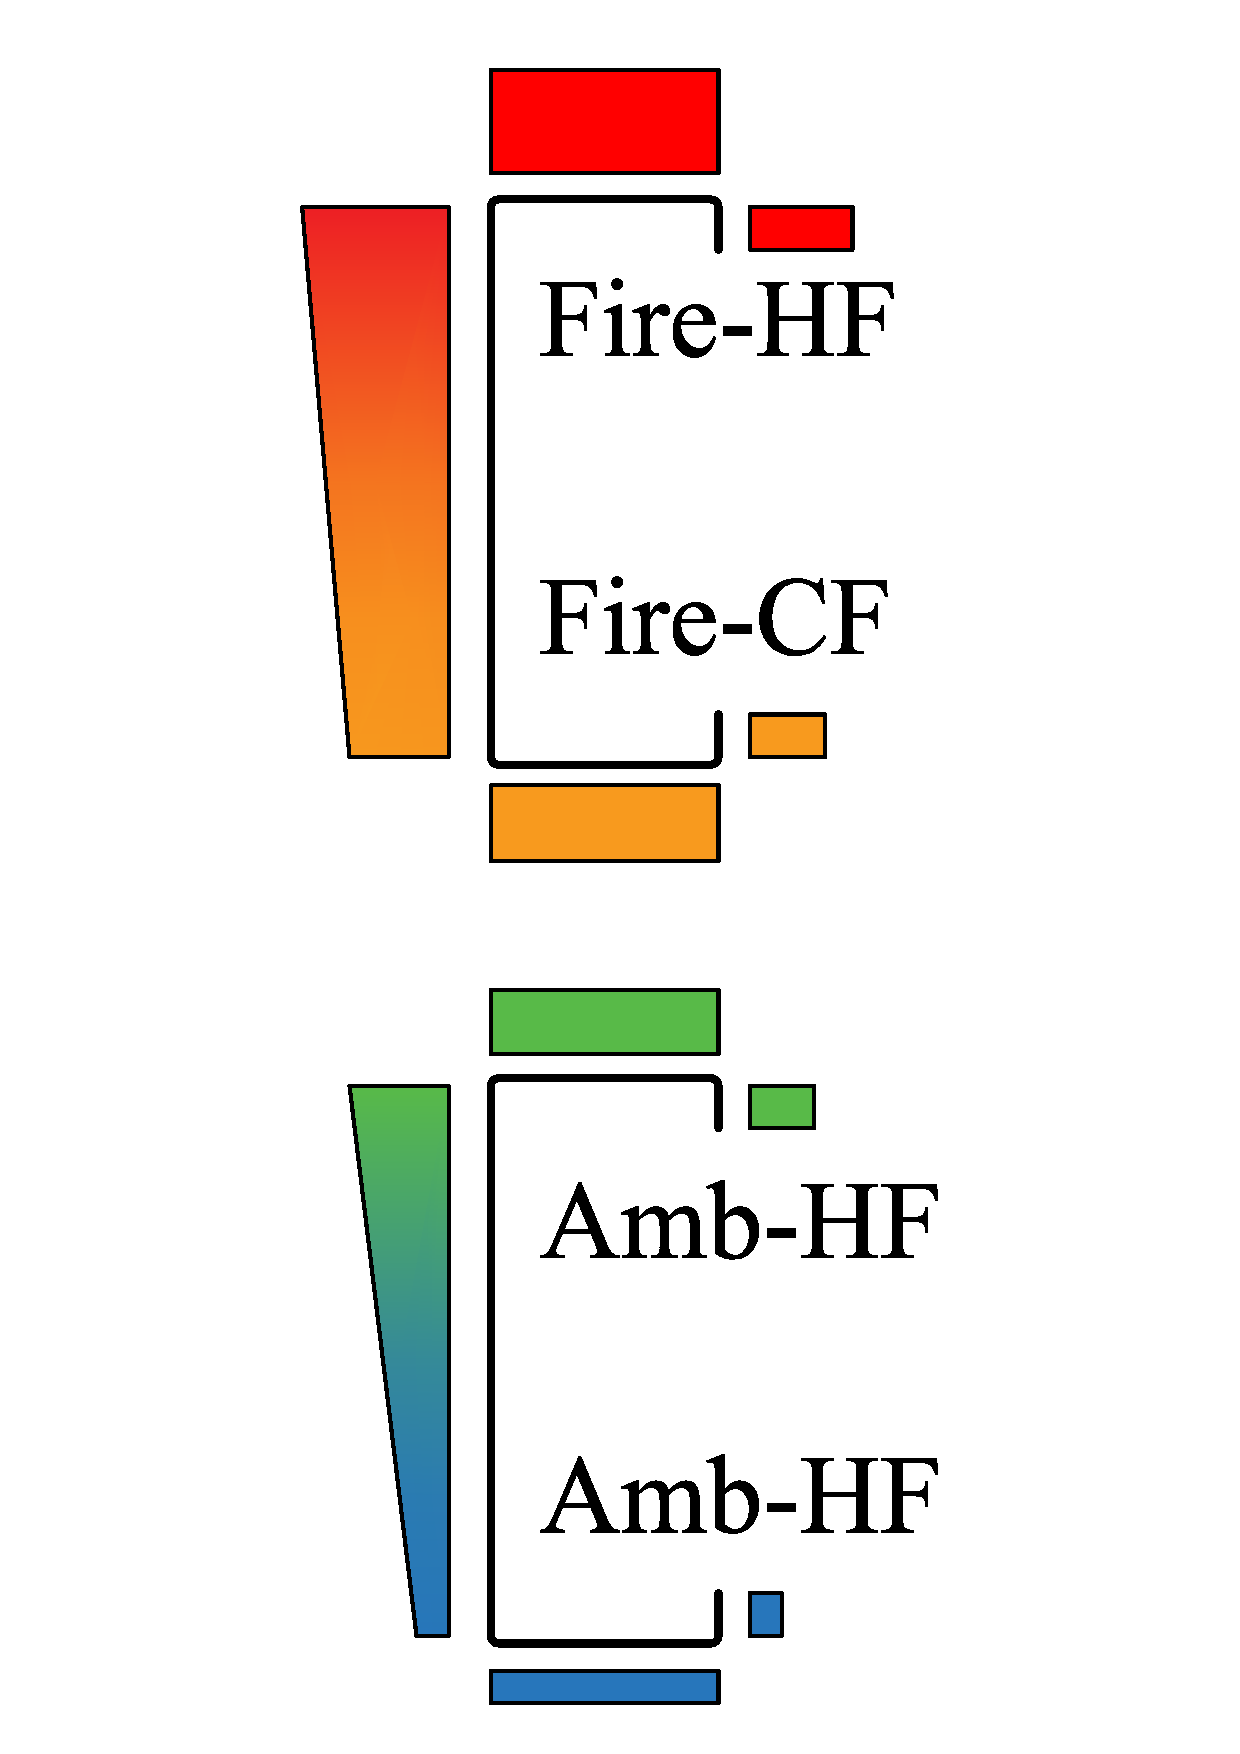
\includegraphics[scale=0.2]{temperature-gradient-stud.pdf}\\
		\caption{Temperature variation of studs in double stud LSF walls}
		\label{fig:temperature-gradient-stud}
\end{figure}
\begin{figure}[!htbp]
	\centering
	\begin{subfigure}[b]{0.7\textwidth}
		\centering
		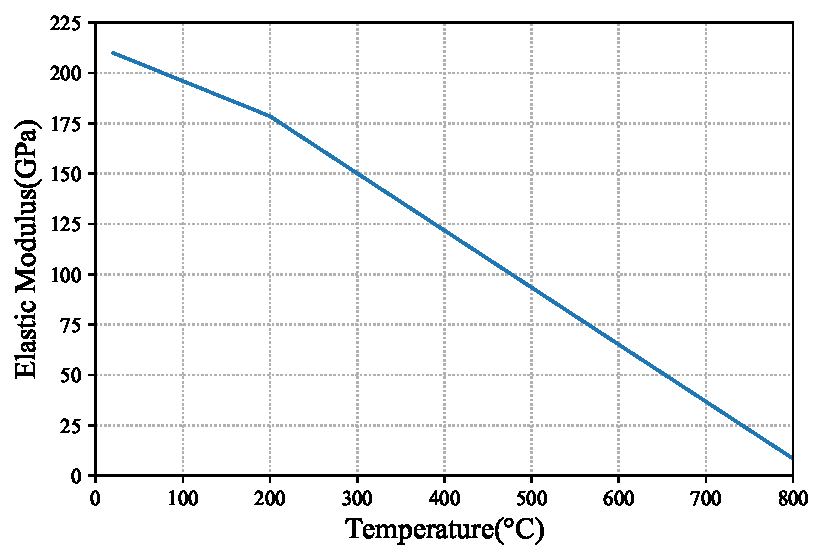
\includegraphics[width=\textwidth]{Steel-elastic-modulus.pdf}
		\caption{}
		\label{subfig:Steel-elastic-modulus}
	\end{subfigure}
	\begin{subfigure}[b]{0.7\textwidth}
		\centering
		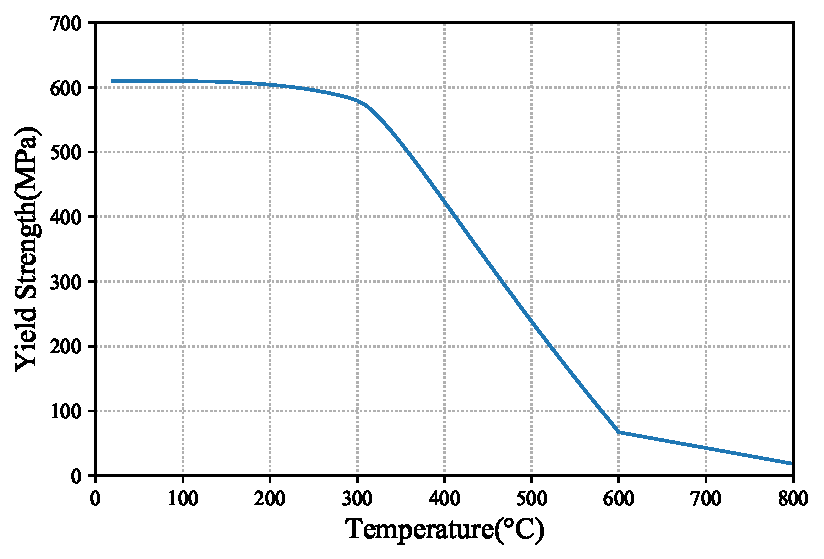
\includegraphics[width=\textwidth]{Steel-yield-strength.pdf}
		\caption{}
		\label{subfig:Steel-yield strength}
	\end{subfigure}
	   \caption{Elevated temperature mechanical properties of G550 steel from \citet{Kankanamge2011}}
	   \label{fig:steel-elevated-mechanical}
\end{figure} 

A coupled-temperature displacement analysis was conducted to determine the structural response of studs under axial compression along with temperature boundary conditions. The applied axial compression load in the FE model was equal to the applied load in the full-scale fire test in \Cref{ch:Fire}. Transient mode of analysis was adapted and all the models were analysed for a time-period of 240 min (14400 s). The effects of non-linearity were considered in the coupled temperature-displacement analysis. This method of structural analysis is generally referred to as sequentially coupled analysis wherein thermal analysis is conducted first followed by structural analysis. The output from thermal analysis acts as input to the structural analysis. The reactions were monitored on the bottom reference point and the axial displacement was monitored on the top reference point of the model at the centroid using history output feature in ABAQUS. The monitored data was stored in an output database file (ODB) and later used for post-processing. 

As the coupled temperature-displacement structural analysis includes the effects of temperatures, the material properties used in the model had to account for the variations caused by elevated temperatures. Therefore, the elevated temperature mechanical properties of cold-formed steel were extracted from \citet{Kankanamge2011} which were verified by \citet{Rokilan2019}. The elevated temperature mechanical properties of steel such as elastic modulus and yield strength used in the FE model are shown in \Cref{fig:steel-elevated-mechanical}. As the coupled-temperature displacement analysis involves solving two boundary conditions such as temperature and axial compression load at the same time, severe convergence issues arise with the FE model. This is because of the non-linear nature of the problem resulting in large deformations in the model. The non-linear nature of the model is largely due to the usage of thin-walled elements as studs. Treating these instabilities with a global solution might not best fit the problem. This was addressed by the introduction of automatic damping factor and adaptive stabilization factor during the analysis. This helps the models to converge to the desired solution. However, as stated earlier in the previous section, determining these factors are based on a trial and error method and varies with the models as stated in the ABAQUS documentation manual (\cite{abaqus2017}). Therefore, the failure criteria of a model is determined either by comparing the reduction in the applied axial load with respect to time or with respect to axial displacement or with lateral deflection or a combination of the aforesaid. The selection of the failure criteria in the FE model depends on the convergence achieved in the given model based on the temperature boundary condition and applied axial loads. 

\section*{Test-T1}

Test-T1 was conducted on a non-cavity insulated double stud LSF wall with 90 $\times$ 0.95 mm lipped channel studs as shown in \Cref{fig:T1-plan-FEA}. Ambient temperature capacity FE model gave an ultimate compression capacity of 71.97 kN. As the full-scale fire Test-T1 was conducted under 0.4 LR (load ratio) an axial compression capacity of 28.76 kN was applied to the model and a coupled temperature displacement analysis was carried out. 
\begin{figure}[!htbp]
	\centering
			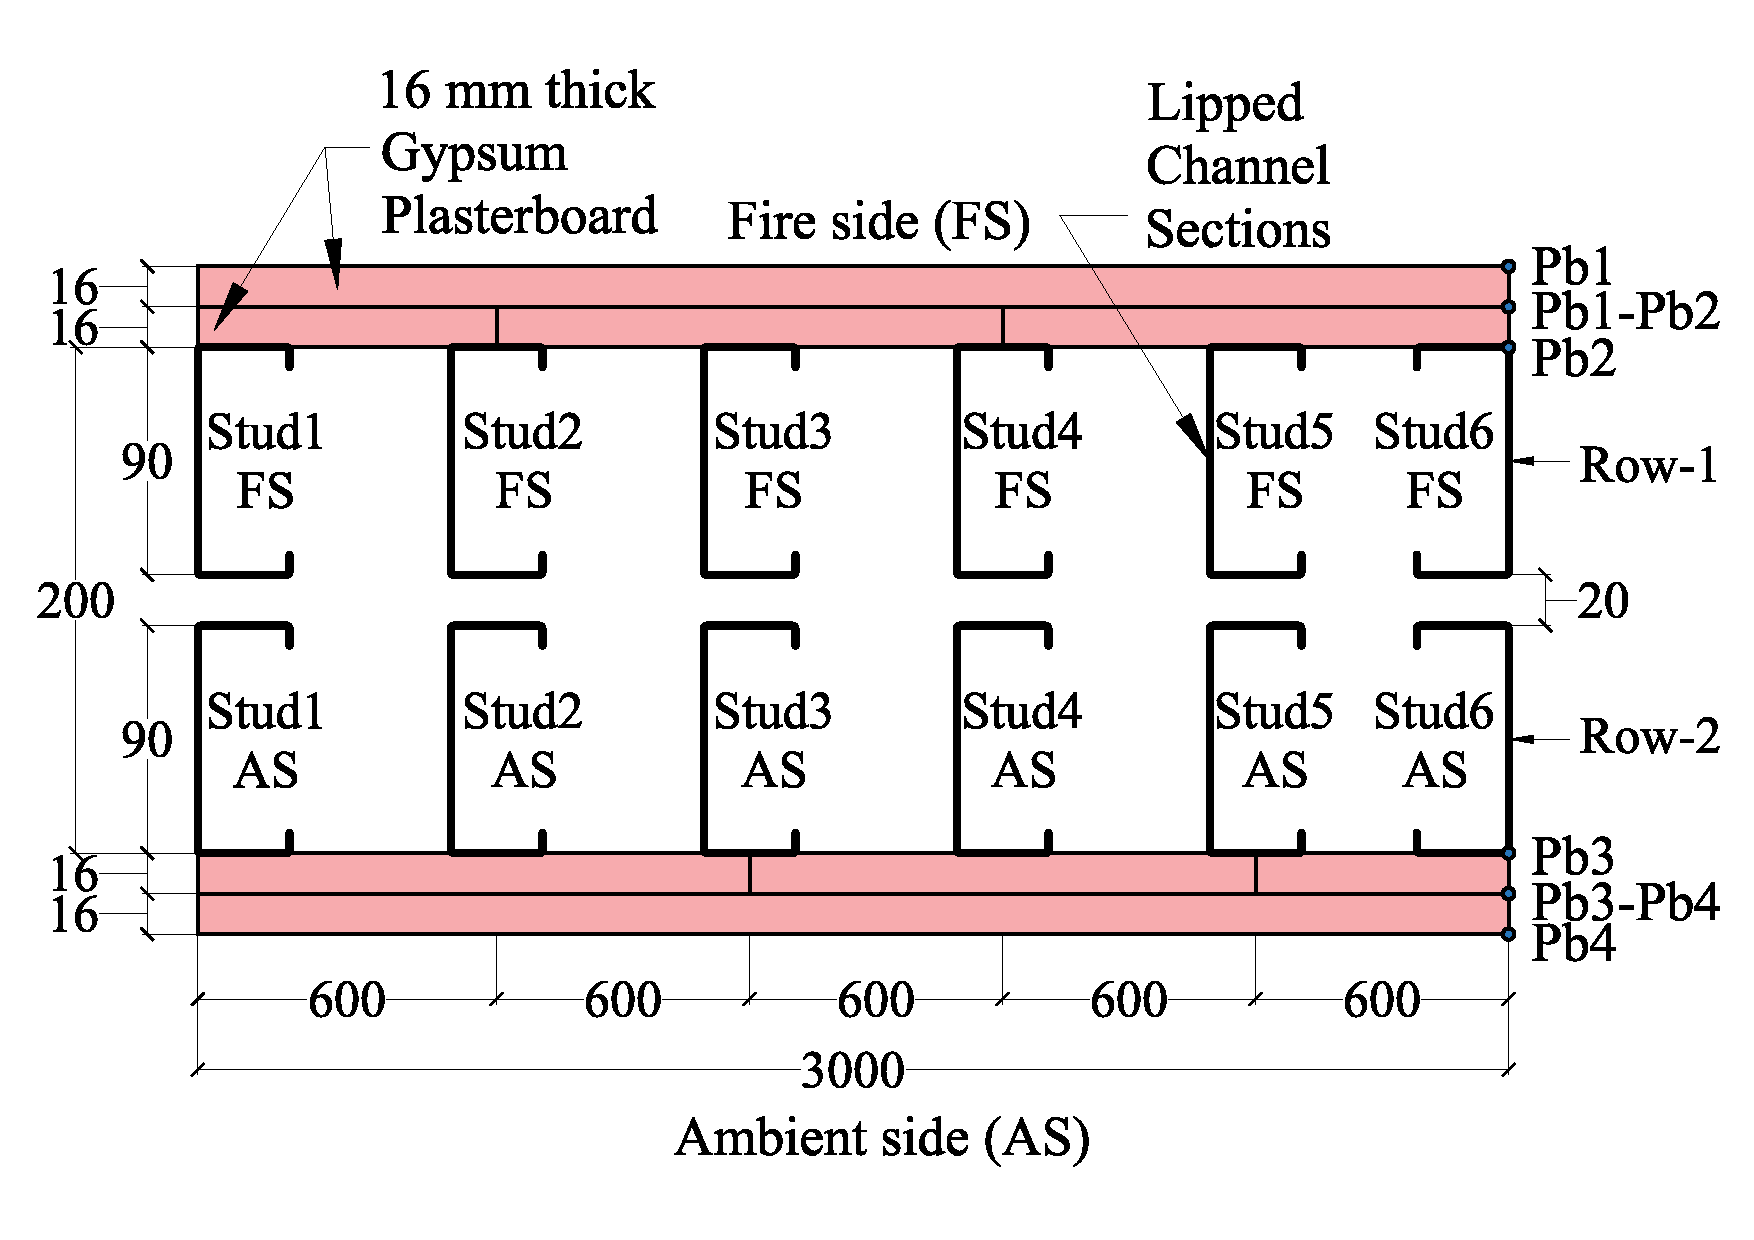
\includegraphics[scale=0.4]{T1-plan.pdf}\\
		\caption{Test-T1 wall configuration}
		\label{fig:T1-plan-FEA}
\end{figure}

To determine the level of agreement in predicting the failure time of the developed structural model, the stud time-temperature curve from Test-T1 was used as boundary condition to the FE model and sequentially coupled temperature-displacement analysis was conducted. The failure of the coupled temperature displacement model of Test-T1 wall was determined using the time versus axial displacement and lateral deflection curves extracted from the model as shown in \Cref{fig:T1-structural-FE-vs-Exp-exp-temp}. The failure time predicted by the FE model was 176 min, which matches accurately with the experimental failure time of 176 min. 

Buckling failure mode extracted from the FE model is shown in \Cref{subfig:T1-buckling-FEA-exp-temp}. The local buckling experienced in the stud hot flanges shown in \Cref{subfig:T1-buckling-FEA-Exp-exp-temp} was simulated by the developed structural FE model as shown in \Cref{subfig:T1-buckling-FEA-exp-temp}. However, the buckling deformation in the hot flange of the stud predicted by the developed structural model was less in comparison with that observed in the experiment. This is attributed to the post-buckling behaviour experienced by the test wall. During fire test, once the limiting hot flange temperature is reached under the applied axial load, the test wall fails due to the buckling failure in studs. However, the application of load to the test wall could not be stopped instantaneously as the load application was controlled manually due to the limitation in the test set-up. This results in excessive buckling deformation of the failed studs in the test wall. In the structural FE model, the coupled temperature-displacement analysis is automatically terminated once convergence is achieved in the model. This may lead to termination of the analysis even before the stud enters the post-ultimate failure phase. Therefore, capturing the post-ultimate failure effects in the FE model is challenging in sequentially coupled-temperature displacement analysis. Generally, altering the stabilization factors in the coupled temperature displacement analysis can result in good predictions of the post-ultimate failure behaviour of the thin-walled steel studs, but might not always result in accurate predictions due to converge issues in the FE model.
\begin{figure}[!htbp]
	\centering
	\begin{subfigure}[b]{0.7\textwidth}
		\centering
		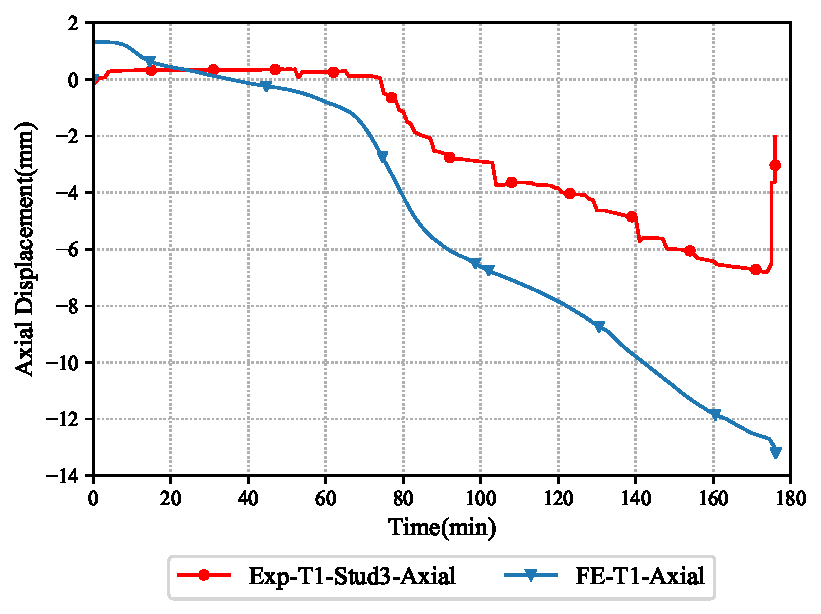
\includegraphics[width=\textwidth]{T1-axial-FE-vs-Exp-exp-temp.pdf}
		\caption{}
		\label{subfig:T1-axial-FE-vs-Exp-exp-temp}
	\end{subfigure}
	\begin{subfigure}[b]{0.7\textwidth}
		\centering
		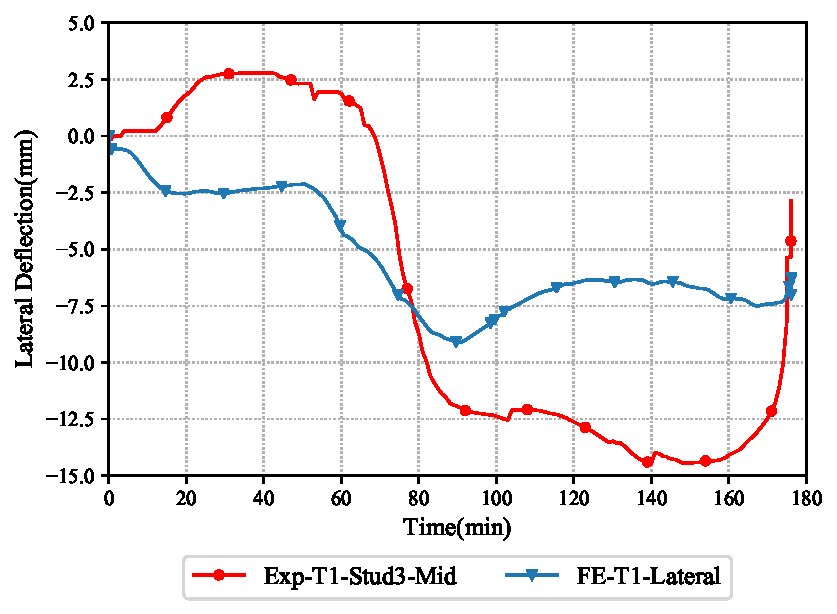
\includegraphics[width=\textwidth]{T1-lateral-FE-vs-Exp-exp-temp.pdf}
		\caption{}
		\label{subfig:T1-lateral-FE-vs-Exp-exp-temp}
	\end{subfigure}
	   \caption{Comparison of displacement versus time curves of Test-T1 from FEA based on stud flange temperatures from experiment and experimental results (a) Axial displacement versus time (b) Lateral deflection versus time curves}
	   \label{fig:T1-structural-FE-vs-Exp-exp-temp}
\end{figure} 
\begin{figure}[!htbp]
	\centering
	\begin{subfigure}[b]{0.85\textwidth}
		\centering
		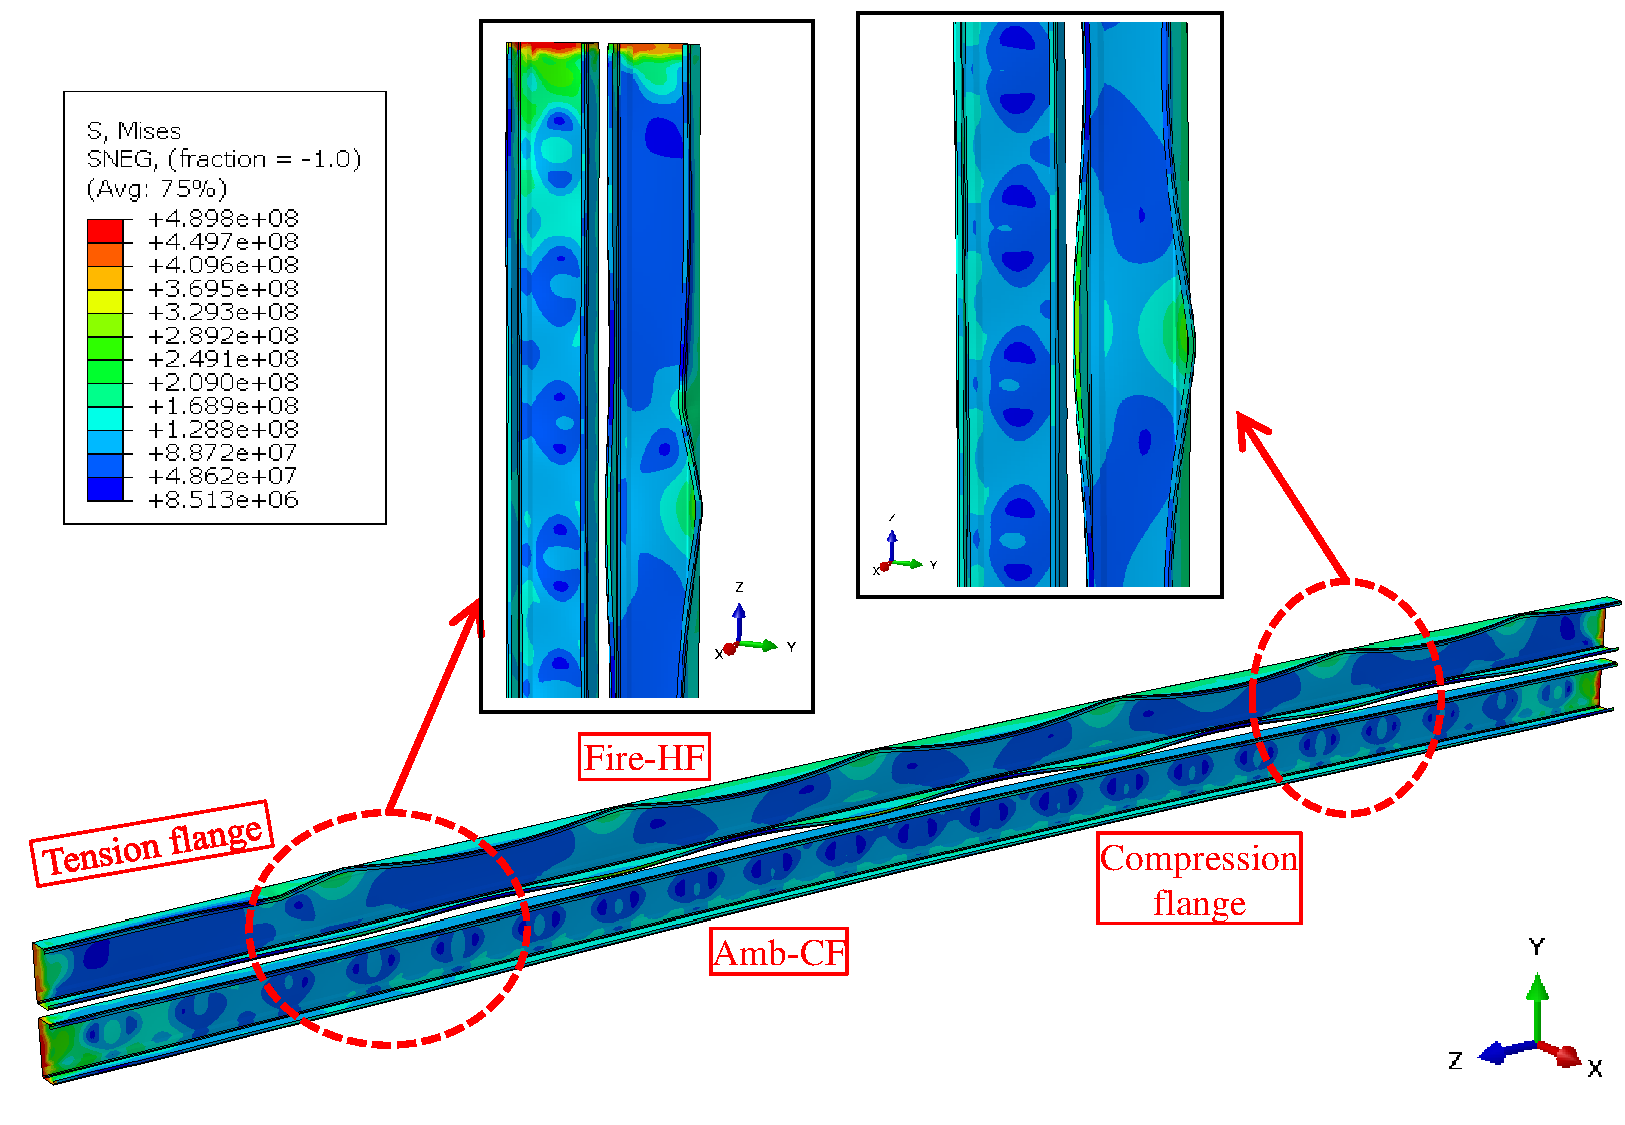
\includegraphics[width=\textwidth]{T1-buckling-FEA-exp-temp.pdf}
		\caption{}
		\label{subfig:T1-buckling-FEA-exp-temp}
	\end{subfigure}
	\begin{subfigure}[b]{0.55\textwidth}
		\centering
		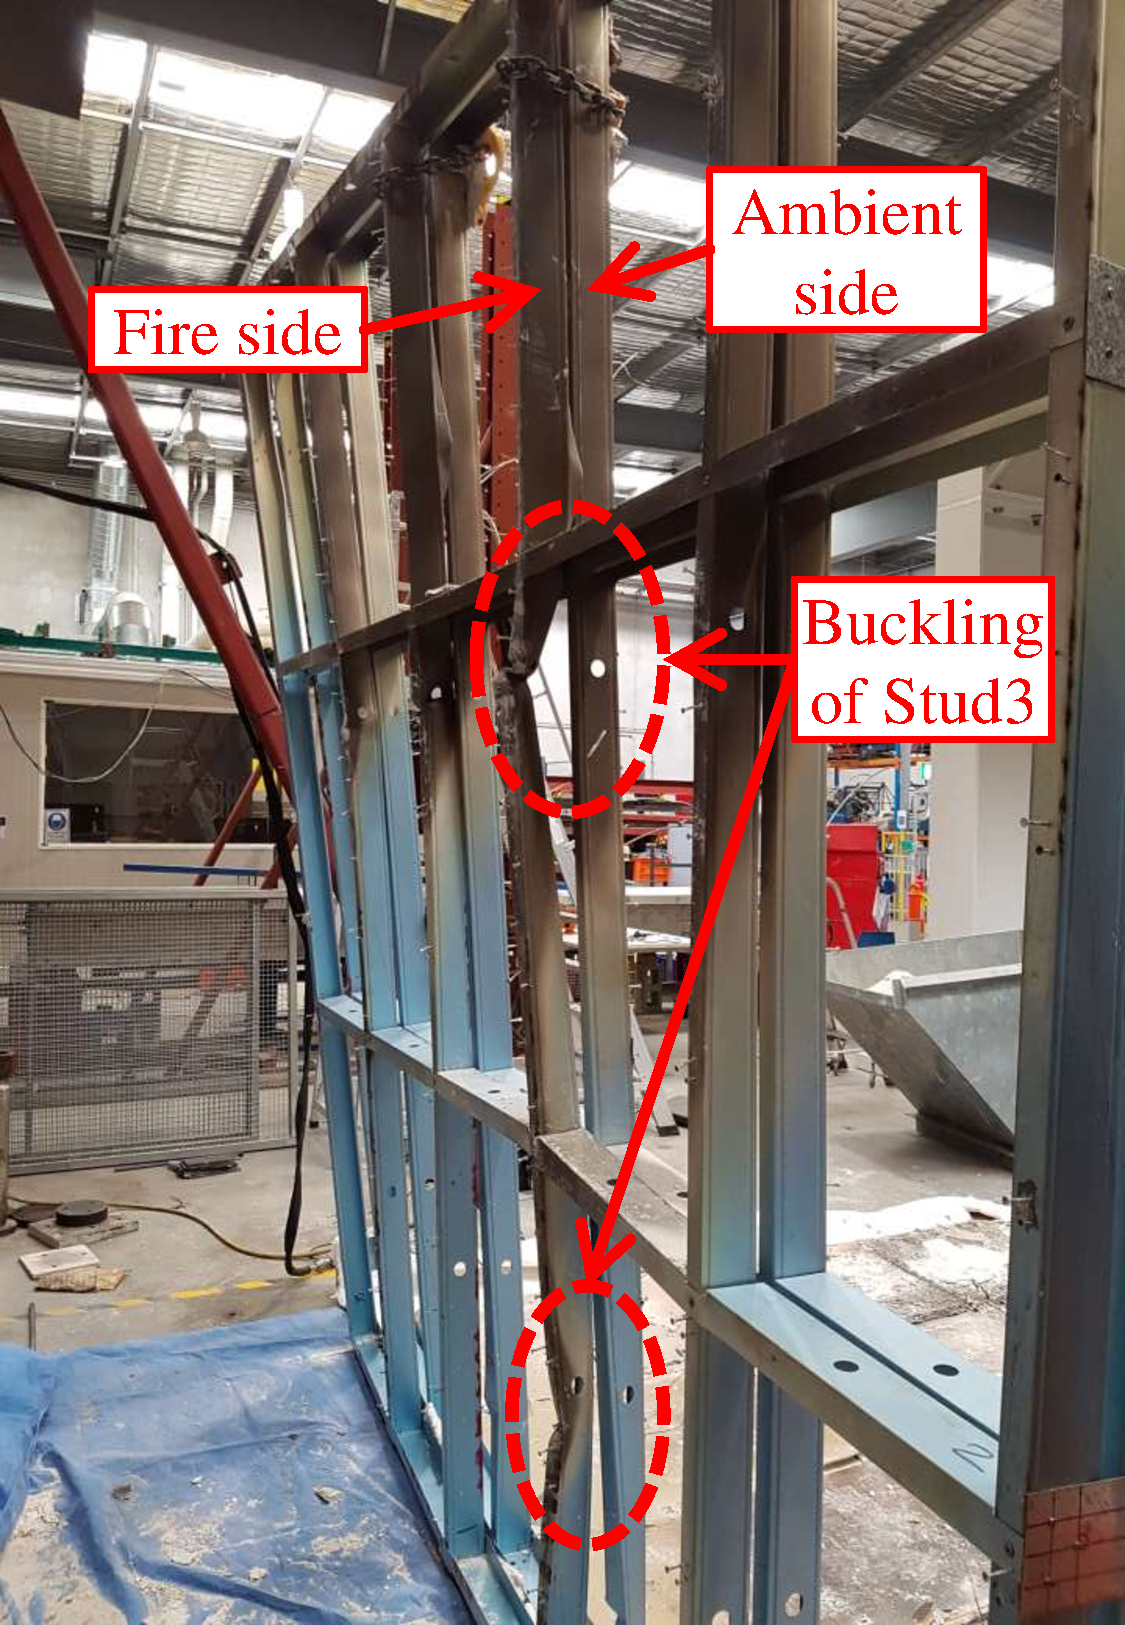
\includegraphics[width=\textwidth]{T1-buckling.pdf}
		\caption{}
		\label{subfig:T1-buckling-FEA-Exp-exp-temp}
	\end{subfigure}
	   \caption{Buckling failure of studs in Test-T1 wall (a) FEA based on stud temperatures from experiment (b) Experiment}
	   \label{fig:T1-buckling-FE-vs-Exp-exp-temp}
\end{figure} 
\begin{figure}[!htbp]
	\centering
	\begin{subfigure}[b]{0.7\textwidth}
		\centering
		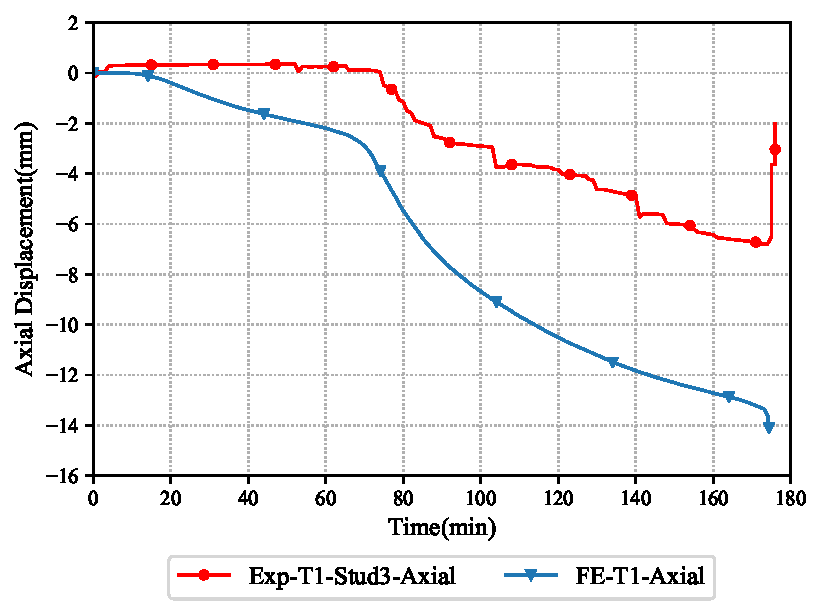
\includegraphics[width=\textwidth]{T1-axial-FE-vs-Exp.pdf}
		\caption{}
		\label{subfig:T1-axial-FE-vs-Exp}
	\end{subfigure}
	\begin{subfigure}[b]{0.7\textwidth}
		\centering
		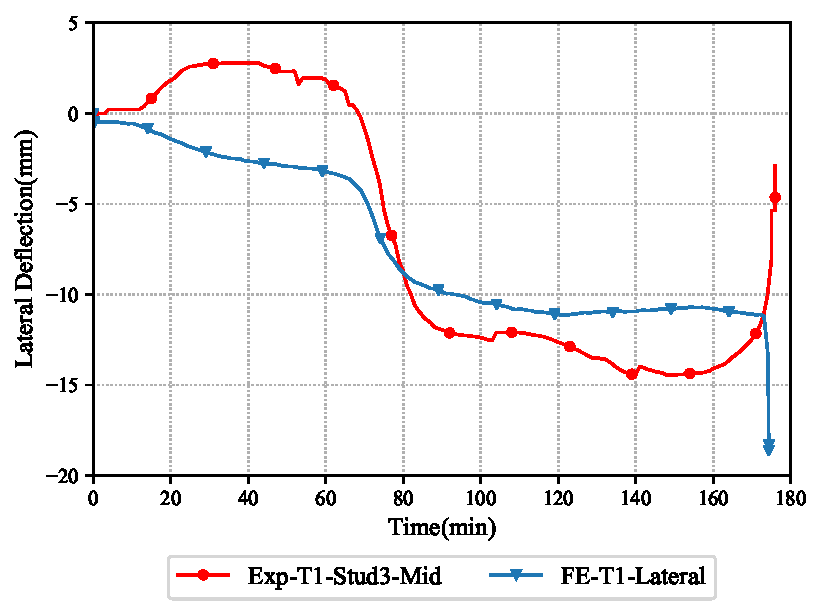
\includegraphics[width=\textwidth]{T1-lateral-FE-vs-Exp.pdf}
		\caption{}
		\label{subfig:T1-lateral-FE-vs-Exp}
	\end{subfigure}
	   \caption{Comparison of displacement versus time curves of Test-T1 from FEA based on stud flange temperatures from FDS and experiment (a) Axial displacement versus time (b) Lateral deflection versus time curves}
	   \label{fig:T1-structural-FE-vs-Exp-exp-temp-disp}
\end{figure} 
\begin{figure}[!htbp]
	\centering
	\begin{subfigure}[b]{0.85\textwidth}
		\centering
		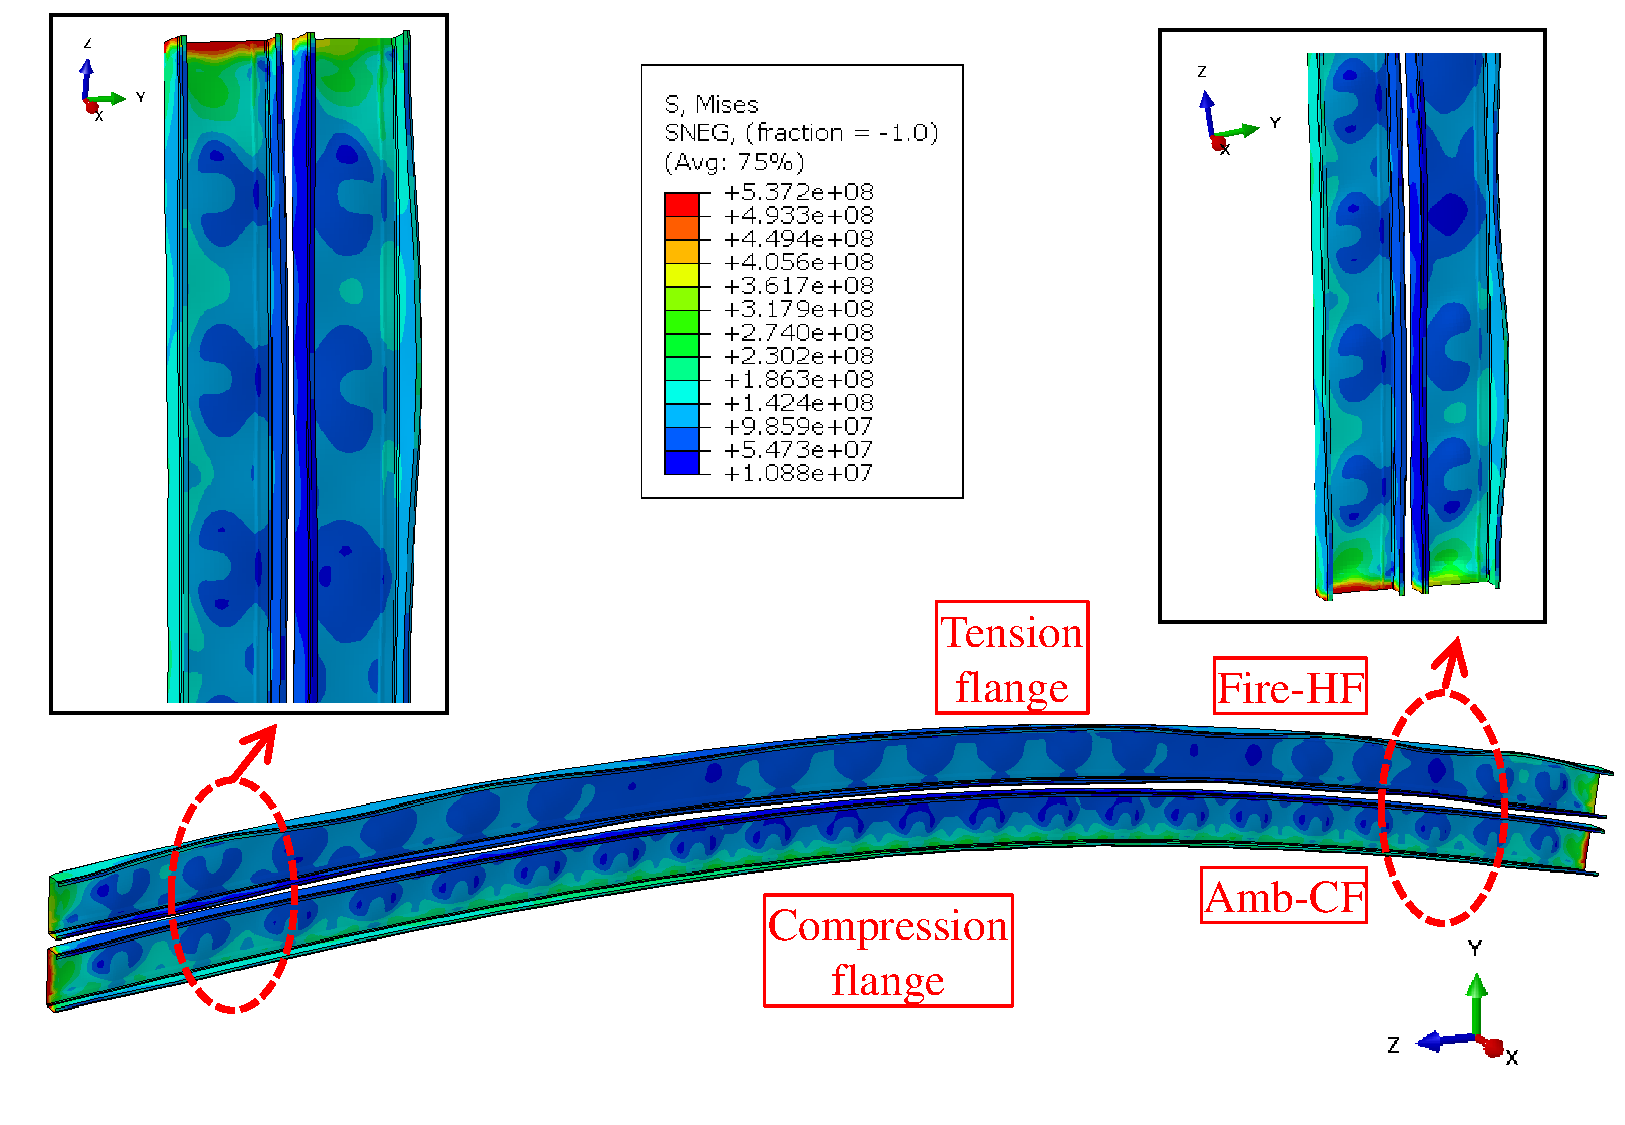
\includegraphics[width=\textwidth]{T1-buckling-FEA.pdf}
		\caption{}
		\label{subfig:T1-buckling-FEA}
	\end{subfigure}
	\begin{subfigure}[b]{0.55\textwidth}
		\centering
		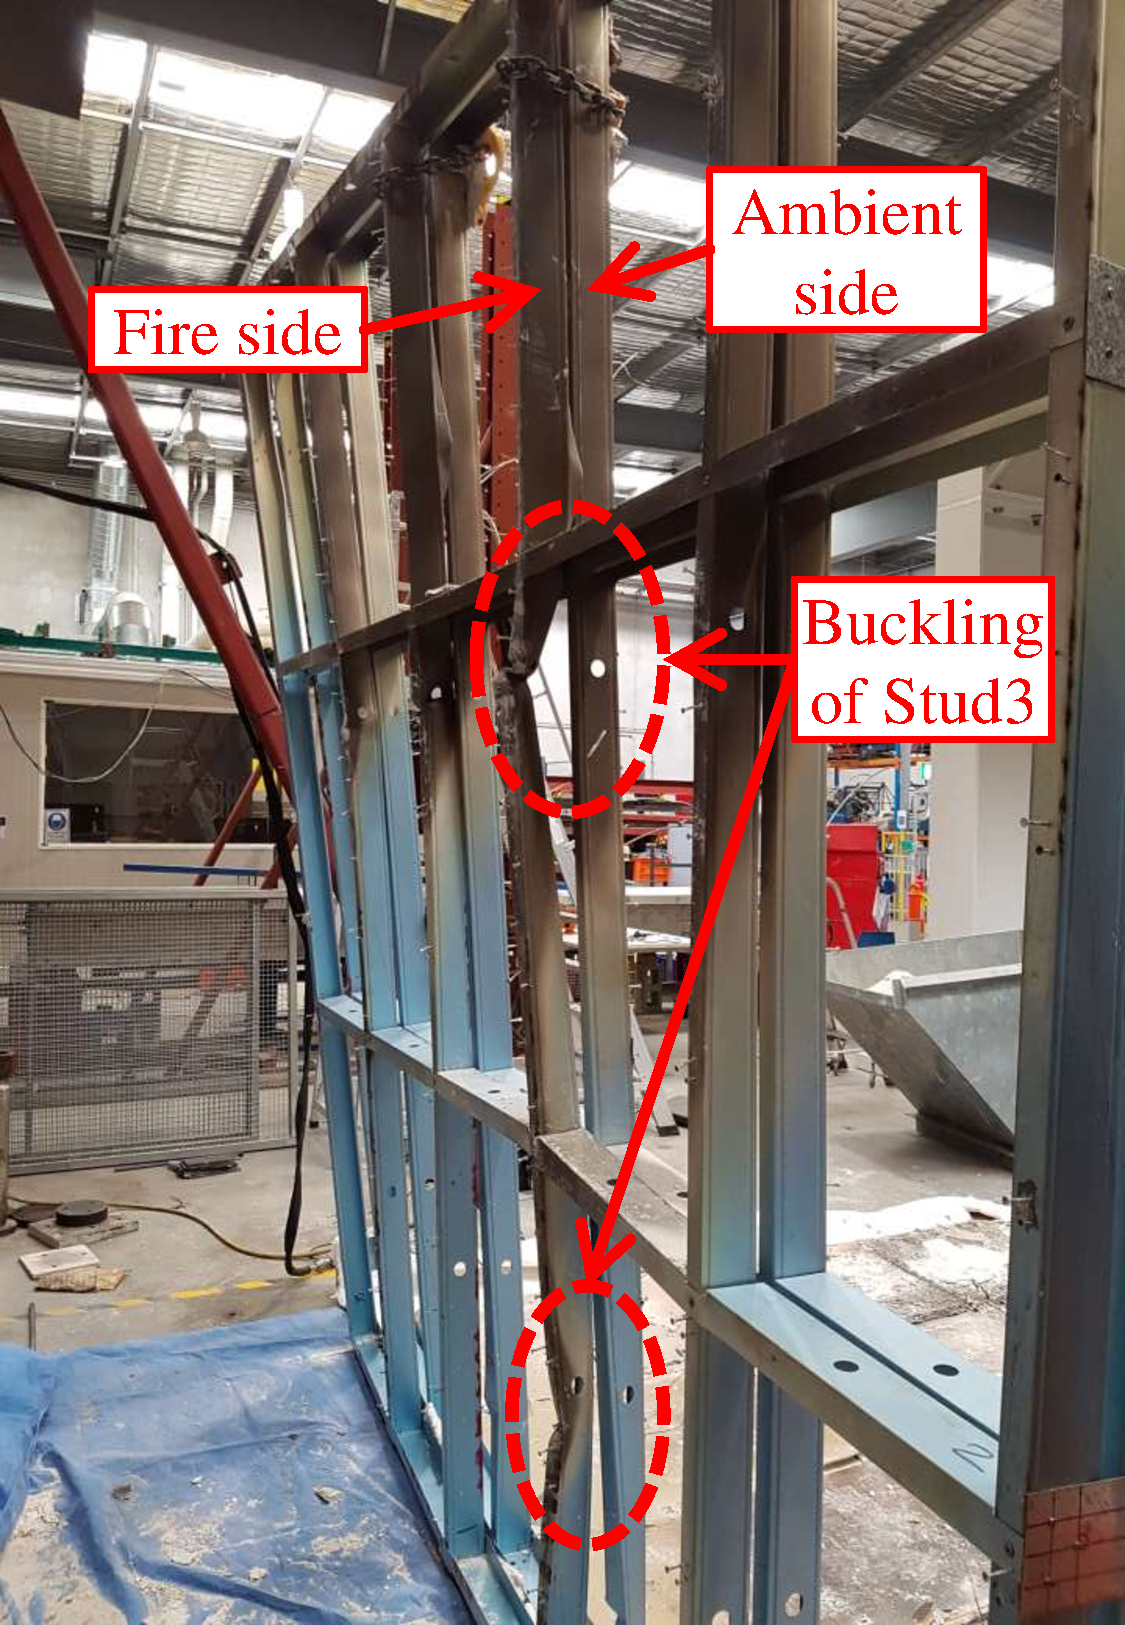
\includegraphics[width=\textwidth]{T1-buckling.pdf}
		\caption{}
		\label{subfig:T1-buckling-FEA-Exp}
	\end{subfigure}
	   \caption{Buckling failure of studs in Test-T1 wall (a) FEA based on stud flange temperatures from FDS (b) Experiment}
	   \label{fig:T1-buckling-FE-vs-Exp}
\end{figure} 

As the developed structural FE model was able to predict the failure time based on the stud temperatures from experiments, attempts were made to incorporate the stud temperature predictions from the FDS model into the structural FE model to predict the failure time for Test-T1. \Cref{fig:T1-structural-FE-vs-Exp-exp-temp-disp} shows the comparison of axial displacement and lateral deflection curves from FE model based on stud temperatures from FDS thermal analysis output and the experimental results. Comparison with the buckling modes from experimental result in \Cref{subfig:T1-buckling-FEA-Exp} reveals that the local buckling of studs observed in the full-scale fire test could not be predicted by the developed FE model. This was due to severe instability in the model causing convergence issue. However, the axial displacement and lateral deflection versus time curves could predict the failure time reasonably well. The failure time predicted by the structural FE model was 174 min while the experiment gave a failure time of 176 min. The maximum axial displacement recorded in the fire Test-T1 was -8 mm while it was 12.75 mm from the FE model predictions. Likewise, the experiment resulted a lateral deflection of -14.44 mm while the FE model gave 18.6 mm.   

\section*{Test-T2}

Test-T2 was conducted on a non-cavity insulated double stud LSF wall similar to the configuration shown in \Cref{fig:T1-plan-FEA} but with thinner lipped channel studs (90 $\times$ 0.75 mm) under 0.4 LR. The axial compression capacity under ambient temperature conditions from FEA was 46.25 kN. Structural analysis for Test-T2 was carried out with an axial compression load of 18.5 kN, representing 0.4 LR. The axial displacement and lateral deflection versus time curves from FEA corresponding to Test-T2 are compared against experimental results in \Cref{fig:T2-structural-FE-vs-Exp}. The axial displacement versus time curve from experiment shows no significant variation for the initial 70 min. However, the predictions from FEA shows a gradual increase in the curve as shown in \Cref{subfig:T2-axial-FE-vs-Exp}. The axial displacement curve is steep after 70 min in both experimental and FEA cases. A sudden increase in the curve at failure witnessed in the experimental curve could also be predicted by the developed structural FE model. The maximum axial displacement recorded from the experiment was 7.13 mm while it was 13.11 mm from the FE model prediction. \Cref{subfig:T2-lateral-FE-vs-Exp} compares the lateral deflection versus time curves from experiment and FEA. The flat region in the lateral deflection curve till 60 min from the experiment was also observed in the FE model prediction. However, the maximum lateral deflection reported in the experiment was larger from the experiment resulting -20.25 mm while it was -16.56 mm from the FE model prediction. Failure time from the FE model prediction was 174 min while it was 132 min from the experiment. This difference in failure time prediction is because of the premature plasterboard fall-off in the fire Test-T2 as reported in \Cref{sec:t2-results}.        
\begin{figure}[!htbp]
	\centering
	\begin{subfigure}[b]{0.7\textwidth}
		\centering
		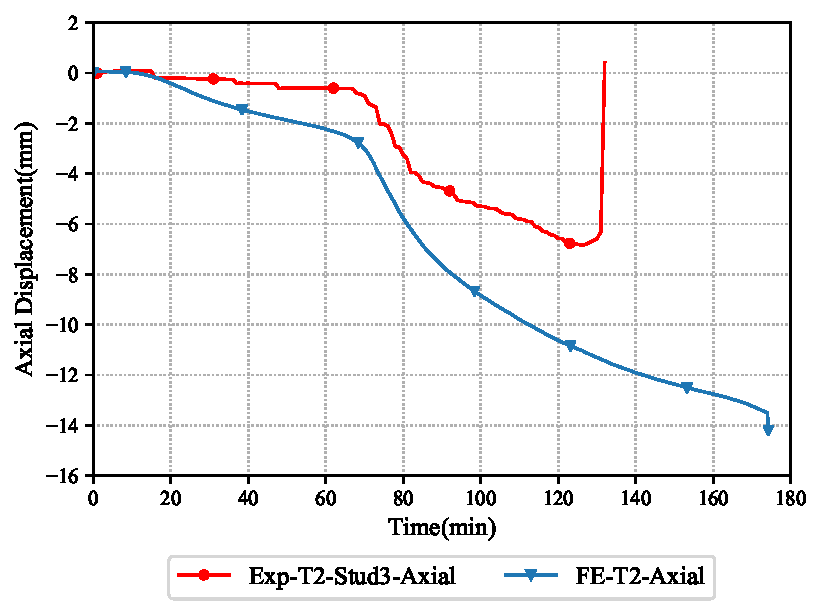
\includegraphics[width=\textwidth]{T2-axial-FE-vs-Exp.pdf}
		\caption{}
		\label{subfig:T2-axial-FE-vs-Exp}
	\end{subfigure}
	\begin{subfigure}[b]{0.7\textwidth}
		\centering
		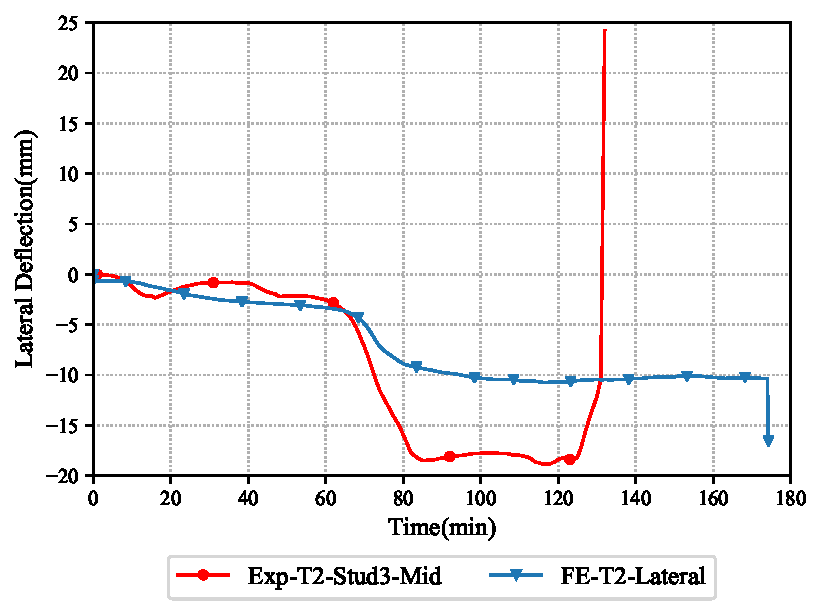
\includegraphics[width=\textwidth]{T2-lateral-FE-vs-Exp.pdf}
		\caption{}
		\label{subfig:T2-lateral-FE-vs-Exp}
	\end{subfigure}
	   \caption{Comparison of displacement versus time curves of Test-T2 from FEA and experiment (a) Axial displacement versus time (b) Lateral deflection versus time curves}
	   \label{fig:T2-structural-FE-vs-Exp}
\end{figure} 
\begin{figure}[!htbp]
	\centering
	\begin{subfigure}[b]{0.85\textwidth}
		\centering
		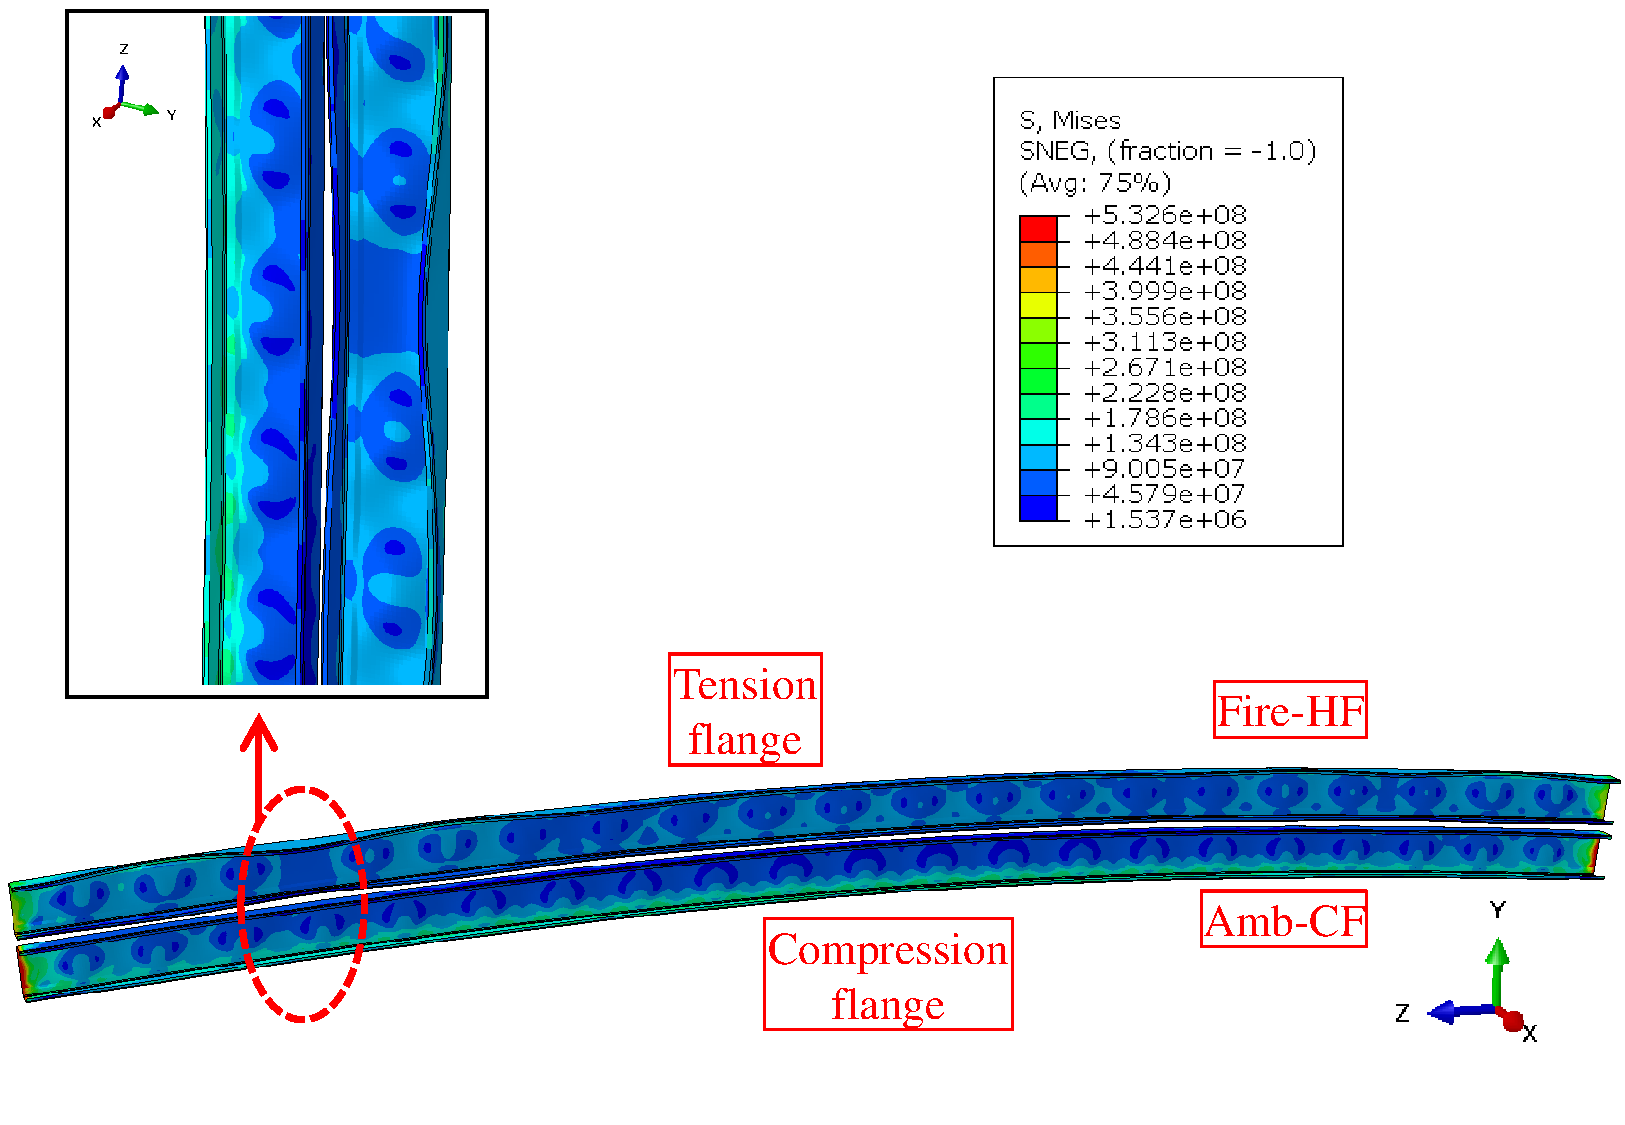
\includegraphics[width=\textwidth]{T2-buckling-FEA.pdf}
		\caption{}
		\label{subfig:T2-buckling-FEA}
	\end{subfigure}
	\begin{subfigure}[b]{0.55\textwidth}
		\centering
		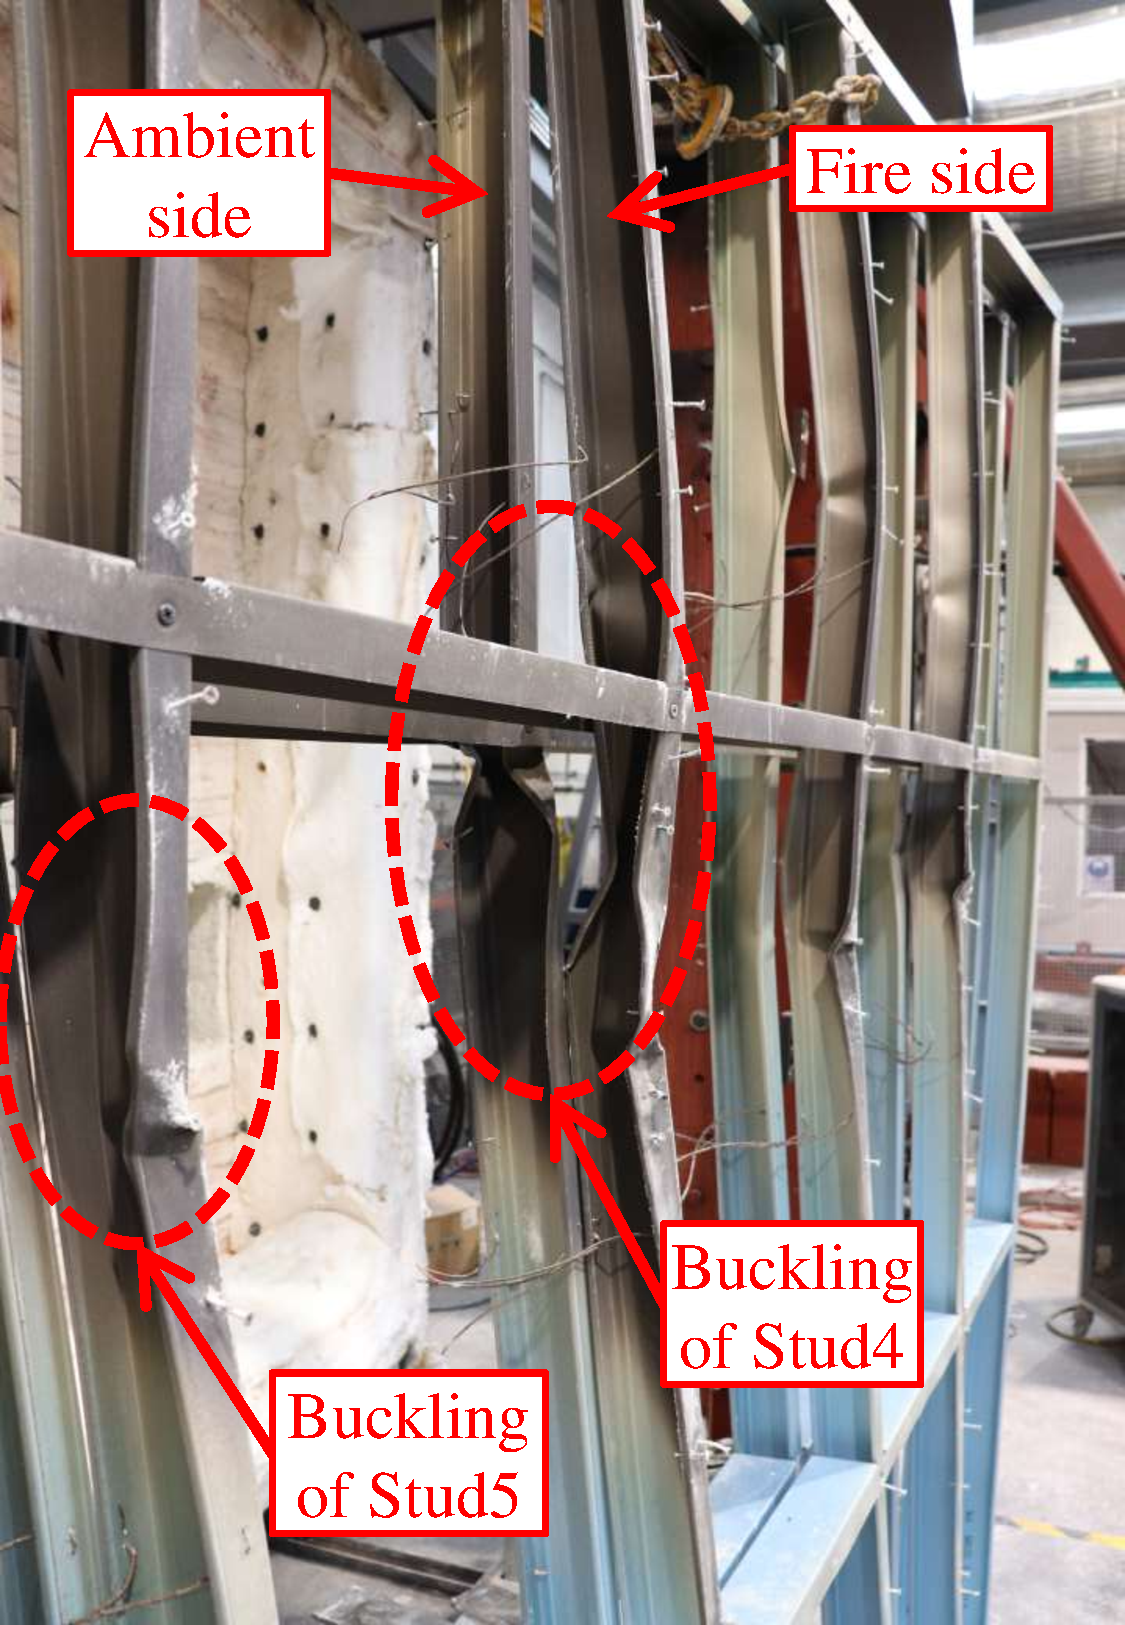
\includegraphics[width=\textwidth]{T2-buckling.pdf}
		\caption{}
		\label{subfig:T2-buckling-FEA-Exp}
	\end{subfigure}
	   \caption{Buckling failure of studs in Test-T2 wall (a) FEA (b) Experiment}
	   \label{fig:T2-buckling-FE-vs-Exp}
\end{figure} 

\Cref{fig:T2-buckling-FE-vs-Exp} shows the comparison of the buckling modes of studs from FE model predictions and experiments. Local buckling was noticeable only on the flanges from the FE model predictions as shown in \Cref{subfig:T2-buckling-FEA} while severe local buckling was noticeable on the stud web and flanges from the experiment as shown in \Cref{subfig:T2-buckling-FEA-Exp}. This was because of the post-failure deformations experienced by the test wall during the full-scale fire test. The FE model experience convergence issues in simulating the post-failure behaviour of the studs thereby resulting in local buckling failure of the flanges corresponding to the failure time as shown in \Cref{subfig:T2-buckling-FEA}.

\section*{Test-T3}

Test-T3 was conducted on a non-cavity insulated double stud LSF wall similar to the configuration shown in \Cref{fig:T1-plan-FEA} with 90 $\times$ 0.75 mm lipped channel studs but under a higher load ratio of 0.6. The axial displacement and lateral deflection versus time curves from FEA and experiment are shown in \Cref{fig:T3-structural-FE-vs-Exp}. The gradual increase in slope exhibited by the axial displacement curve from experiment was also noticeable in the FE predictions as shown in \Cref{subfig:T3-axial-FE-vs-Exp}. The lateral deflection was nearly flat and reached a sudden increase at the end of the fire test. This behaviour in the lateral deflection could also be predicted by the structural FE model as shown in \Cref{subfig:T3-lateral-FE-vs-Exp}. The failure time predicted by the FE model was 82 min compared to that of 81 min from the fire test. The agreement in failure time between the FE model prediction and experimental result was good in Test-T3 as no significant plasterboard fall-off was noticeable in this fire test unlike in Test-T2.
\begin{figure}[!htbp]
	\centering
	\begin{subfigure}[b]{0.7\textwidth}
		\centering
		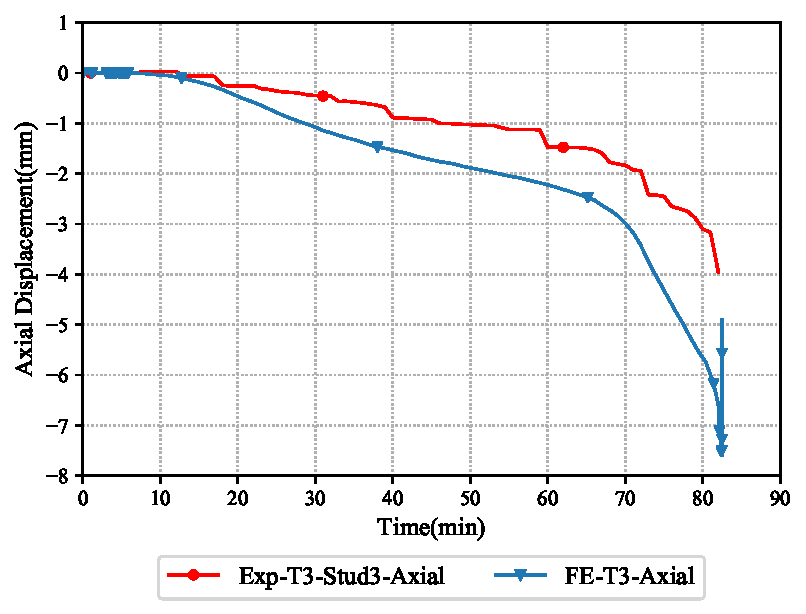
\includegraphics[width=\textwidth]{T3-axial-FE-vs-Exp.pdf}
		\caption{}
		\label{subfig:T3-axial-FE-vs-Exp}
	\end{subfigure}
	\begin{subfigure}[b]{0.7\textwidth}
		\centering
		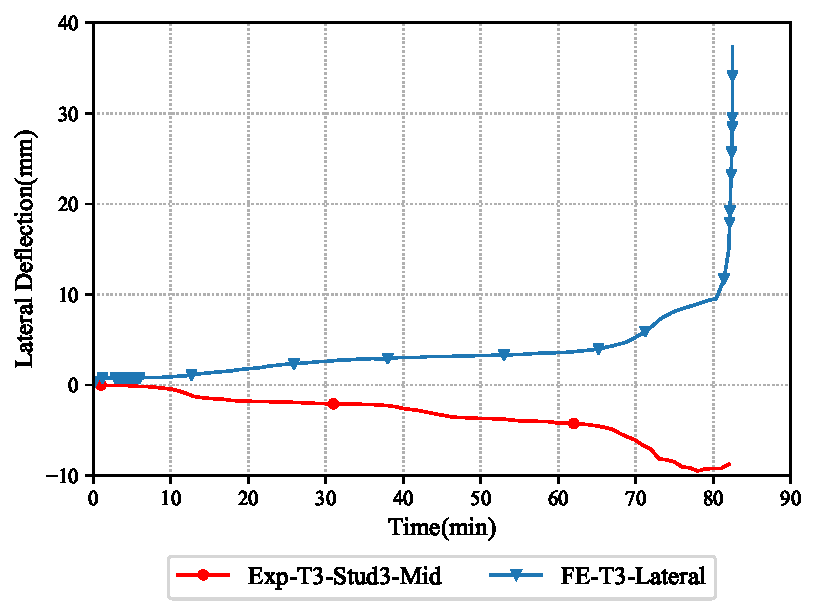
\includegraphics[width=\textwidth]{T3-lateral-FE-vs-Exp.pdf}
		\caption{}
		\label{subfig:T3-lateral-FE-vs-Exp}
	\end{subfigure}
	   \caption{Comparison of displacement versus time curves of Test-T3 from FEA and experiment (a) Axial displacement versus time (b) Lateral deflection versus time curves}
	   \label{fig:T3-structural-FE-vs-Exp}
\end{figure} 
\begin{figure}[!htbp]
	\centering
	\begin{subfigure}[b]{0.85\textwidth}
		\centering
		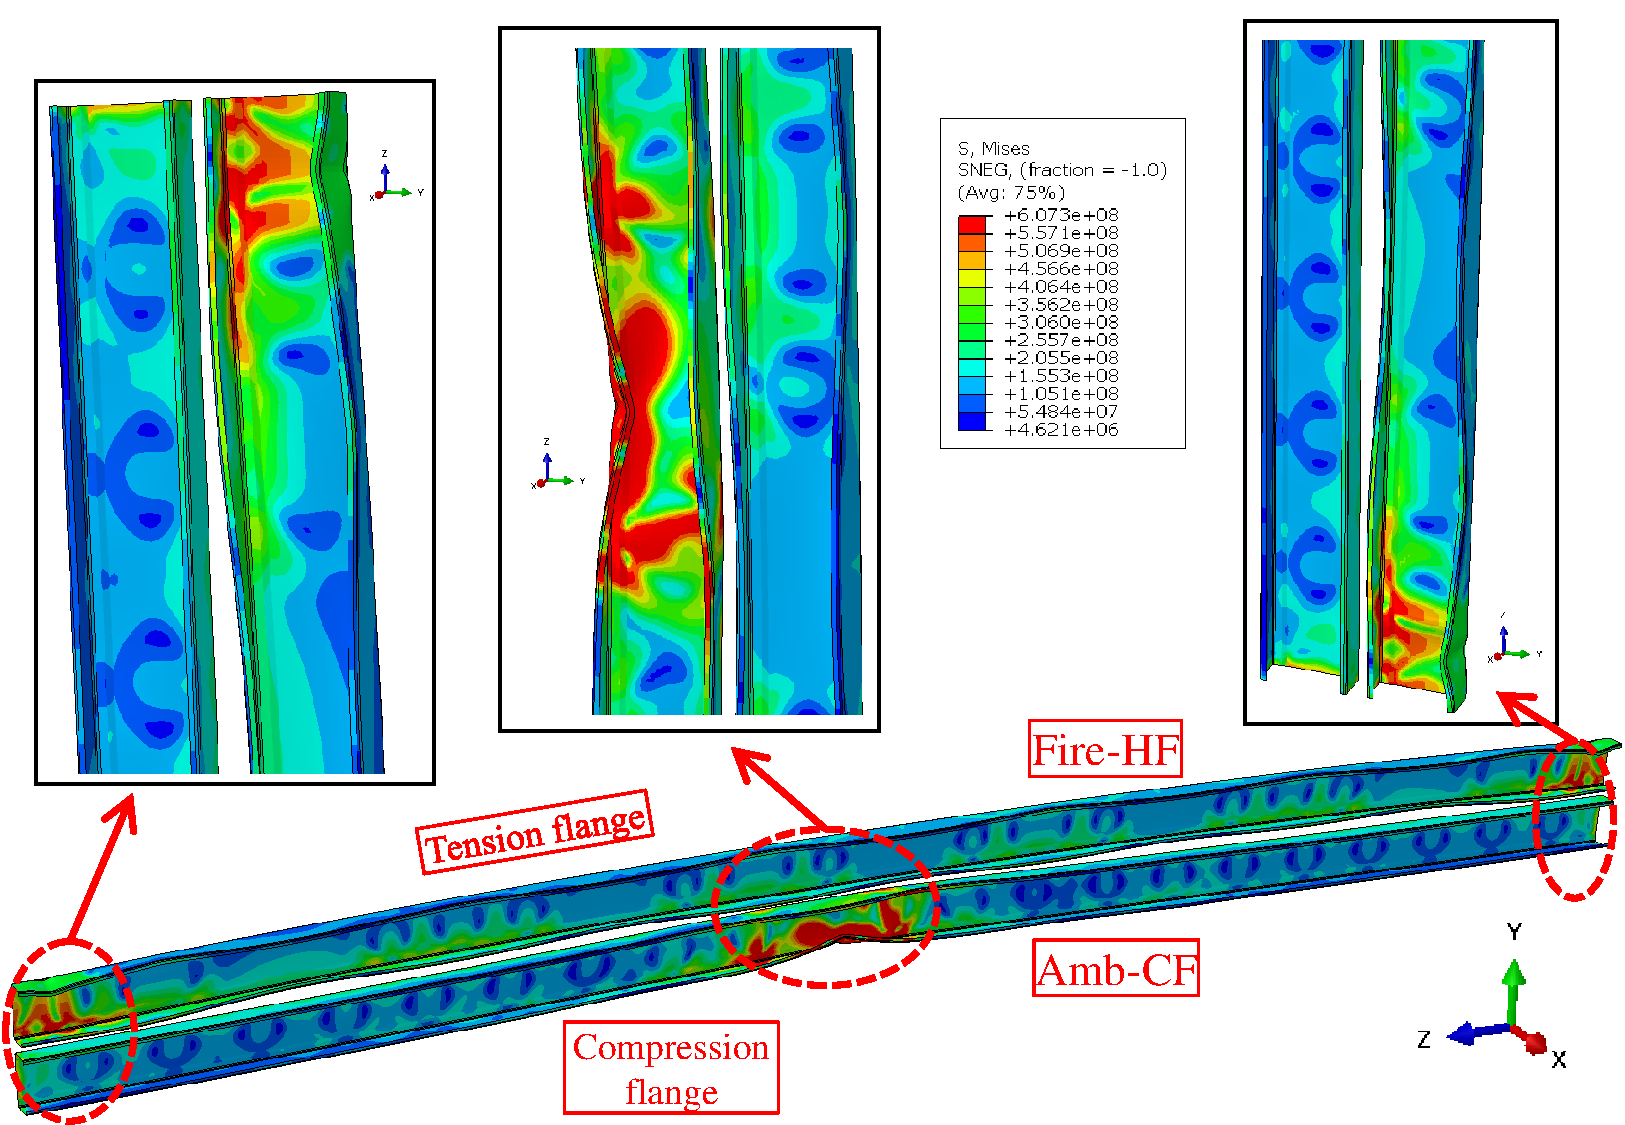
\includegraphics[width=\textwidth]{T3-buckling-FEA.pdf}
		\caption{}
		\label{subfig:T3-buckling-FEA}
	\end{subfigure}
	\begin{subfigure}[b]{0.5\textwidth}
		\centering
		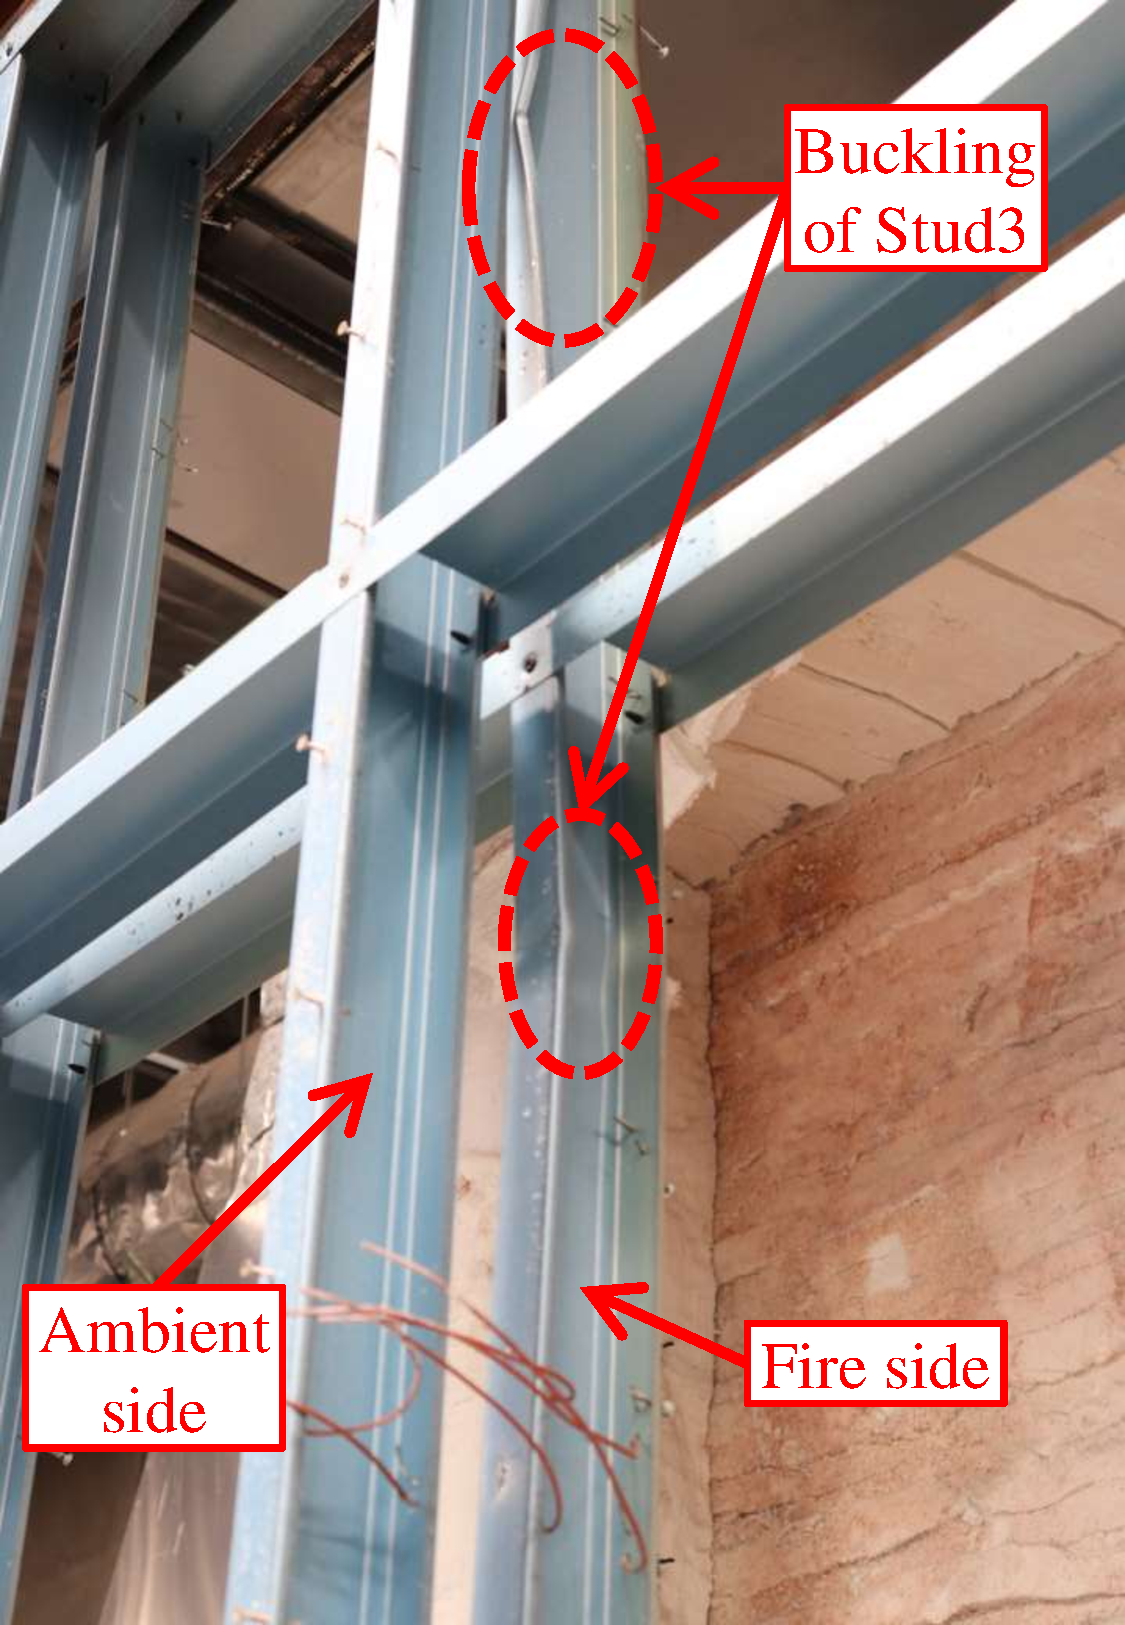
\includegraphics[width=\textwidth]{T3-buckling.pdf}
		\caption{}
		\label{subfig:T3-buckling-FEA-Exp}
	\end{subfigure}
	   \caption{Buckling failure of studs in Test-T3 wall (a) FEA (b) Experiment}
	   \label{fig:T3-buckling-FE-vs-Exp}
\end{figure} 

Local buckling of the flange was the predominant failure mode in the experiment as shown in \Cref{subfig:T3-buckling-FEA-Exp} and was noticed at mid-height in the 3 m test wall. No significant buckling of the web was noticed in the experiment. Similar observations were observed from the FE model simulations. However, the buckling on the fire side stud was noticeable near the ends while the local buckling of the flange at mid-height was noticeable on the ambient side stud. This is because of the load sharing to the ambient side post-failure of the fire side stud which was simulated by the developed structural FE model. The local buckling of flanges near mid-height on the fire side stud in experiment may also be attributed to the localised plasterboard joint open-up in the experiment. Joint open-ups in the test wall could result in localised temperature concentration on the stud fire side hot flange thereby causing localised buckling as witnessed in Test-T3. The plasterboard joint open-up is more susceptible in Test-T3 as the fire test was conducted under higher load ratio.

\section*{Test-T4}

Test-T4 was conducted on a non-cavity insulated double stud LSF wall with 70 $\times$ 0.95 mm studs based on the wall configuration shown in \Cref{fig:T4-plan-FEA}. The axial compression capacity under ambient temperature conditions from FEA was 71.81 kN. Structural analysis for Test-T4 was carried out with an axial compression load of 28.7 kN, representing 0.4 LR. The axial displacement and lateral deflection versus time curves from experiment and FE predictions are compared against each other in \Cref{fig:T4-structural-FE-vs-Exp}. The axial displacement versus time curve from the experiment as shown in \Cref{subfig:T4-axial-FE-vs-Exp} exhibited a flat region till 60 min of fire test after which it progressively increased to a maximum of -5.95 mm at the end of the fire test. This behaviour was also reflected in the structural FE model prediction wherein a maximum axial displacement of 15 mm was recorded at the end of the fire test. The axial displacement versus time curve then changed sign indicating structural failure in the model similar to the experiment. Lateral deflection versus time curve shown in \Cref{subfig:T4-lateral-FE-vs-Exp} also exhibited reasonable agreement between the FE model prediction and the experimental result. The change in slope experienced in the lateral deflection versus time curve after 60 min was also reflected in the FE model prediction. The maximum lateral deflection predicted by the FE model at the time of failure was 19 mm while it was -24.43 mm from the experiment. 
\begin{figure}[!htbp]
	\centering
			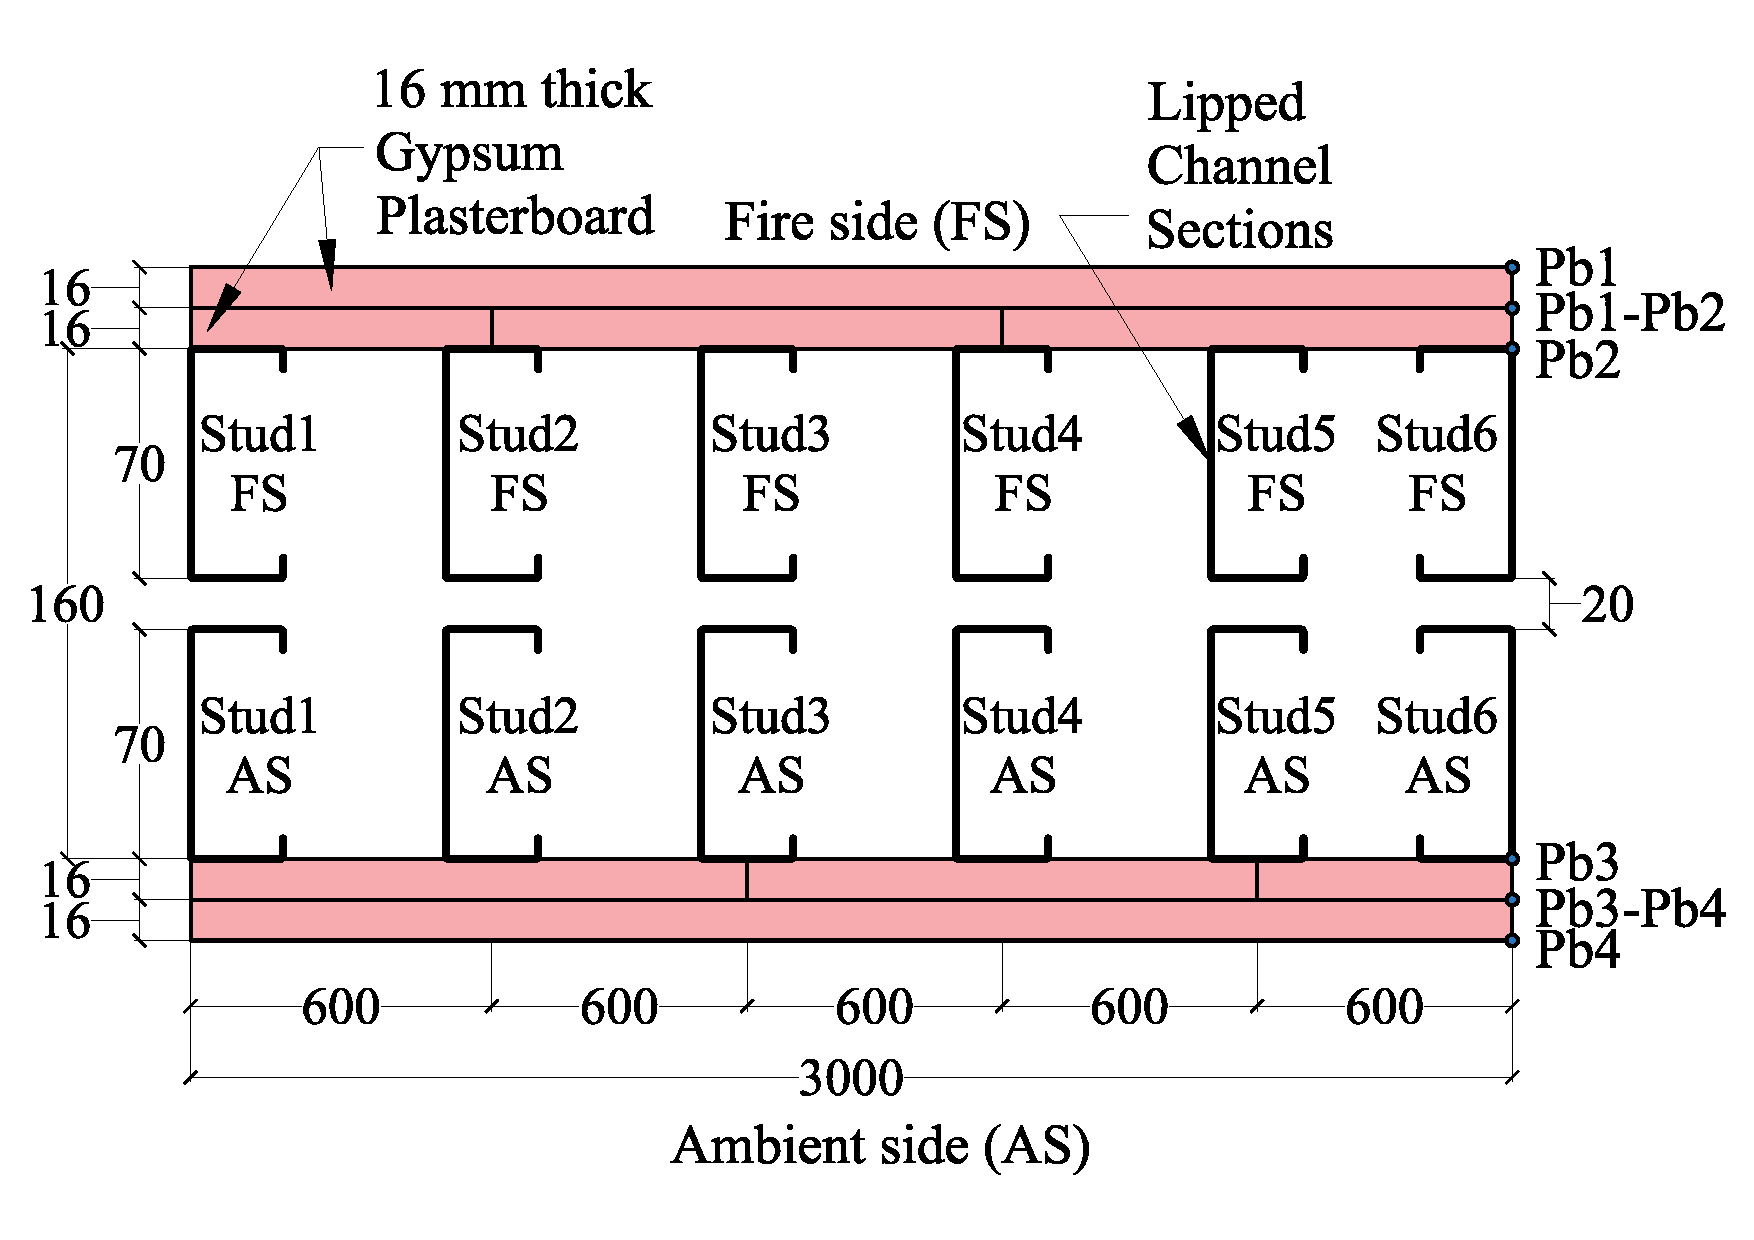
\includegraphics[scale=0.4]{T4-plan.pdf}\\
		\caption{Test-T4 wall configuration}
		\label{fig:T4-plan-FEA}
\end{figure}

The failure time predicted by the FE model was 178 min while it was 171 min from the experiment. Local compressive failure on the fire side hot flange of studs observed in the full-scale fire test could also be simulated by the developed FE model as shown in \Cref{fig:T4-buckling-FE-vs-Exp}. The axial compression load given to the structural FE model was based on the predictions from \Cref{ch:Ambient} where the ambient compression capacity predicted by the ambient structural model was less than the ambient capacity experimental result. When the non-dimensional load ratio is taken for consideration, the failure time prediction for the full-scale fire test matched reasonably well with the experimental failure time for Test-T4. The local buckling of the flanges in the fire side studs was observed at the top of the specimen as shown in \Cref{subfig:T4-buckling-FEA-Exp}. Similar behaviour was simulated by the FE model as shown in \Cref{subfig:T4-buckling-FEA}. This infers that the buckling failure behaviour of the studs in Test-T4 wall could be simulated by the developed FE model considering the stud temperatures from FDS thermal model. 
\begin{figure}[!htbp]
	\centering
	\begin{subfigure}[b]{0.7\textwidth}
		\centering
		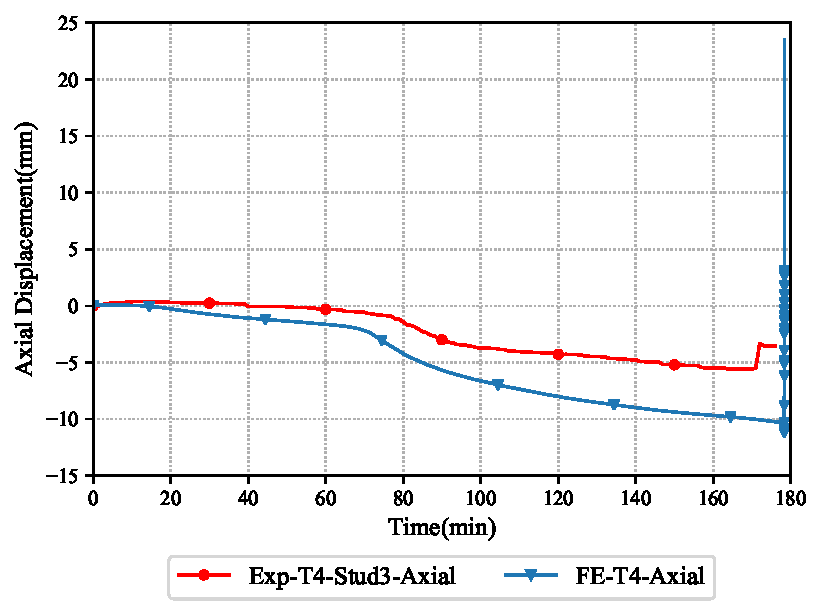
\includegraphics[width=\textwidth]{T4-axial-FE-vs-Exp.pdf}
		\caption{}
		\label{subfig:T4-axial-FE-vs-Exp}
	\end{subfigure}
	\begin{subfigure}[b]{0.7\textwidth}
		\centering
		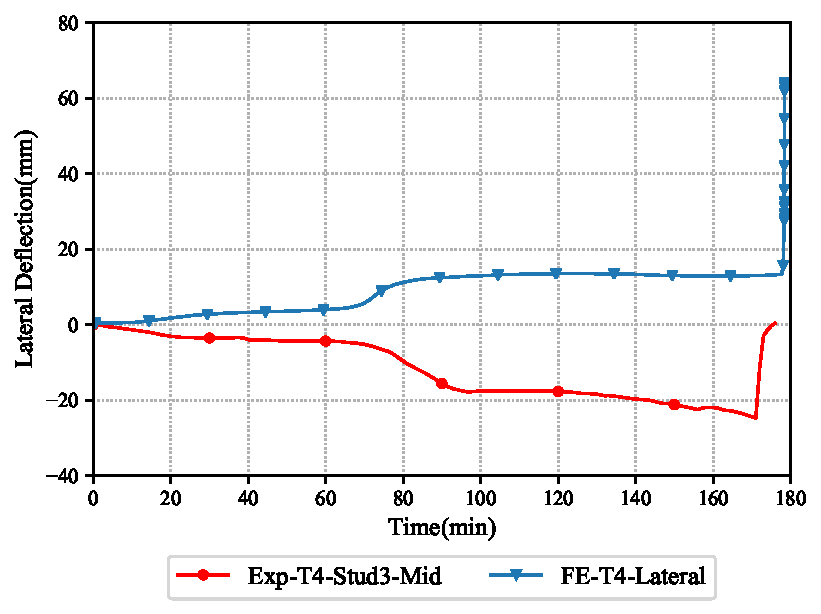
\includegraphics[width=\textwidth]{T4-lateral-FE-vs-Exp.pdf}
		\caption{}
		\label{subfig:T4-lateral-FE-vs-Exp}
	\end{subfigure}
	   \caption{Comparison of displacement versus time curves of Test-T4 from FEA and experiment (a) Axial displacement versus time (b) Lateral deflection versus time curves}
	   \label{fig:T4-structural-FE-vs-Exp}
\end{figure} 
\begin{figure}[!htbp]
	\centering
	\begin{subfigure}[b]{0.85\textwidth}
		\centering
		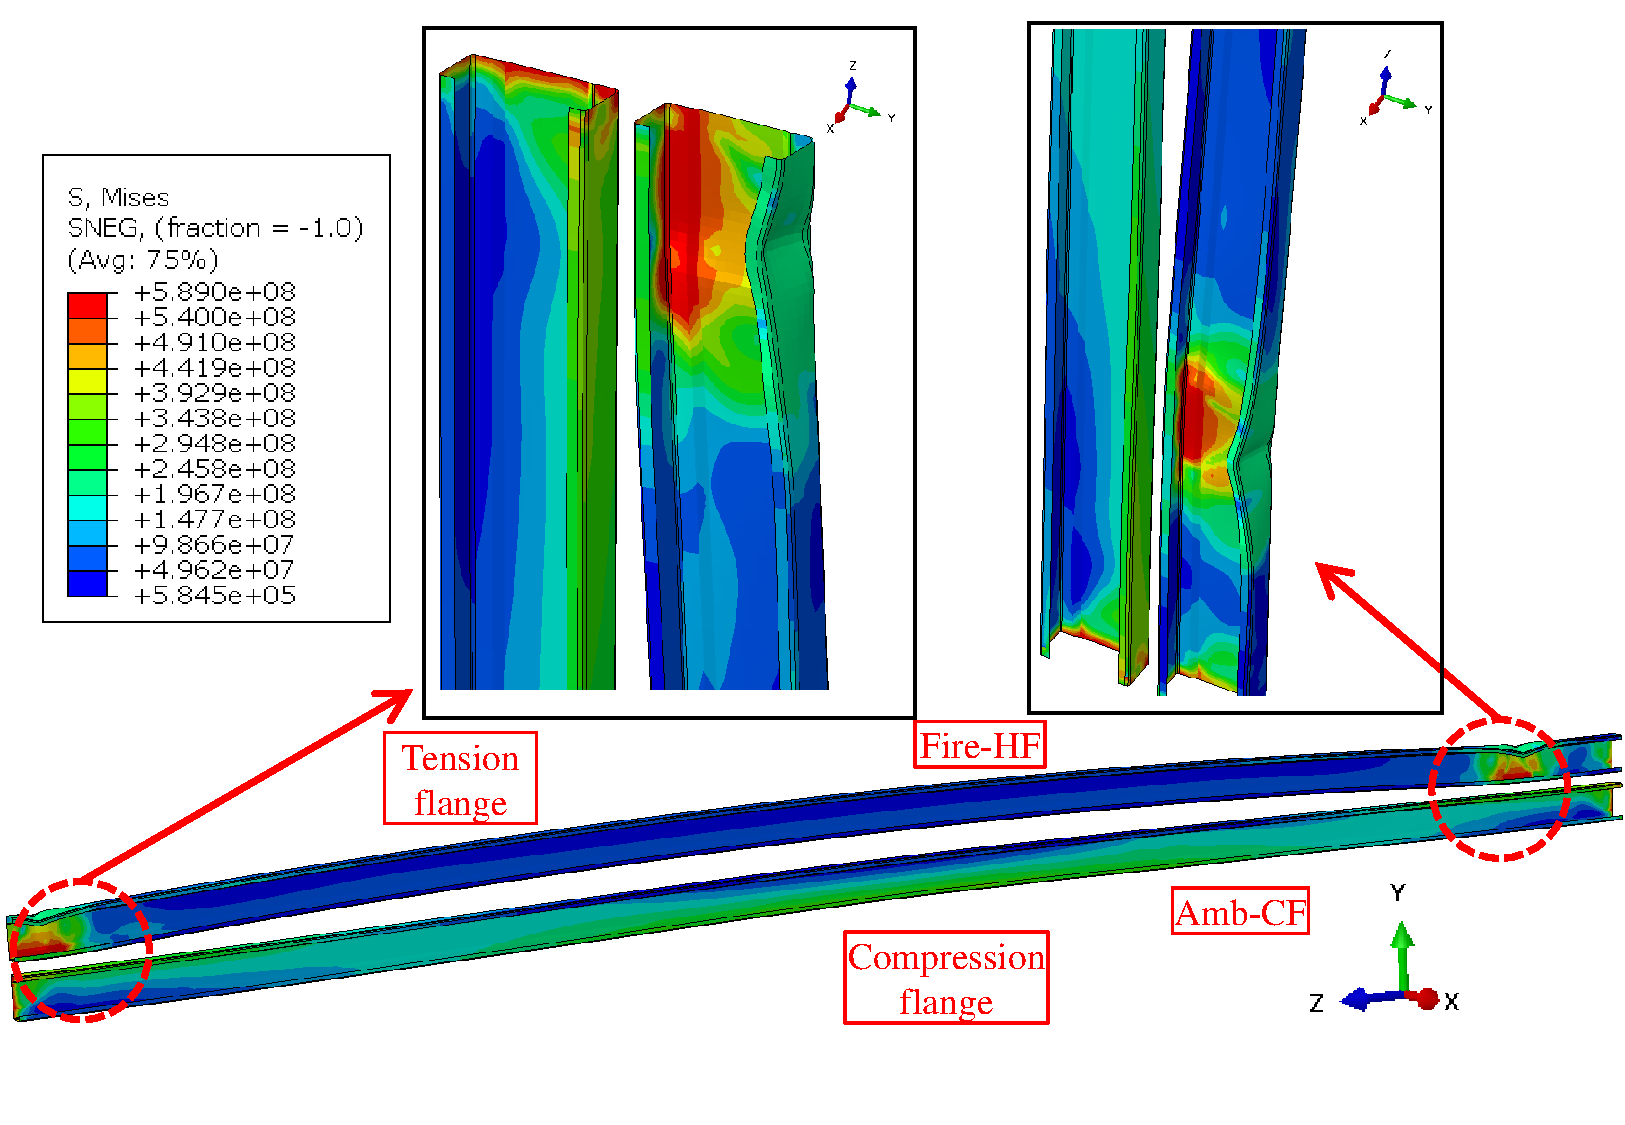
\includegraphics[width=\textwidth]{T4-buckling-FEA.pdf}
		\caption{}
		\label{subfig:T4-buckling-FEA}
	\end{subfigure}
	\begin{subfigure}[b]{0.55\textwidth}
		\centering
		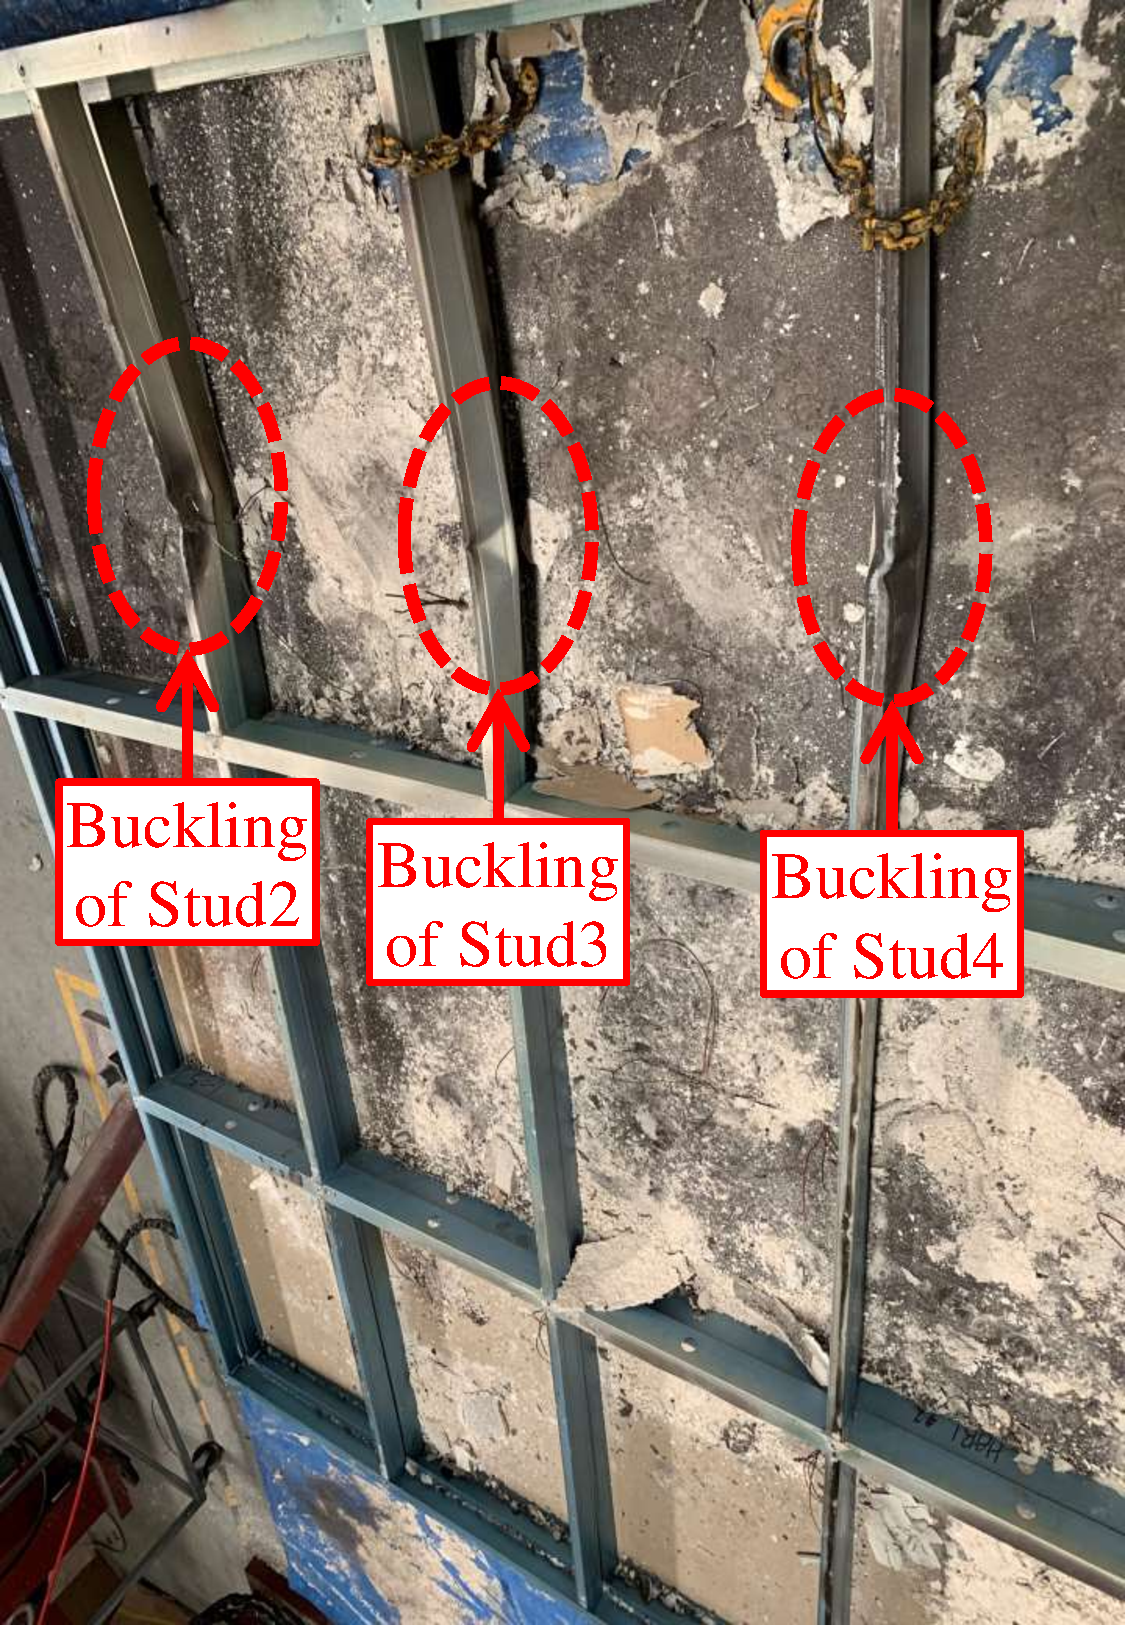
\includegraphics[width=\textwidth]{T4-buckling.pdf}
		\caption{}
		\label{subfig:T4-buckling-FEA-Exp}
	\end{subfigure}
	   \caption{Buckling of studs in Test-T4 wall (a) FEA (b) Experiment}
	   \label{fig:T4-buckling-FE-vs-Exp}
\end{figure} 

\section*{Test-T5}

Test-T5 was conducted on a double stud LSF wall with glass fibre cavity insulation and 90 $\times$ 0.95 mm studs as shown on \Cref{fig:T5-plan-FEA}. The difference between the cavity insulated wall tests in comparison with the non-cavity insulated wall tests is the large temperature difference between the hot and cold flanges. This was also predicted by the developed FDS thermal model as discussed in \Cref{sec:fds-cavity-models} of \Cref{ch:FE-Thermal}. The input boundary conditions of the structural FE models also incorporated these effects. The axial displacement and lateral deflection versus time curves from the structural FE analysis are compared against the experimental results in \Cref{fig:T5-structural-FE-vs-Exp}. Similar to the experimental results of the axial displacement versus time curve in \Cref{subfig:T5-axial-FE-vs-Exp}, FE analysis predicted curve was flat till the end of the fire test simulation. 
\begin{figure}[!htbp]
	\centering
			\includegraphics[scale=0.4]{T5-plan.pdf}\\
		\caption{Test-T5 wall configuration}
		\label{fig:T5-plan-FEA}
\end{figure}
\begin{figure}[!htbp]
	\centering
	\begin{subfigure}[b]{0.7\textwidth}
		\centering
		\includegraphics[width=\textwidth]{T5-axial-FE-vs-Exp.pdf}
		\caption{}
		\label{subfig:T5-axial-FE-vs-Exp}
	\end{subfigure}
	\begin{subfigure}[b]{0.7\textwidth}
		\centering
		\includegraphics[width=\textwidth]{T5-lateral-FE-vs-Exp.pdf}
		\caption{}
		\label{subfig:T5-lateral-FE-vs-Exp}
	\end{subfigure}
	   \caption{Comparison of displacement versus time curves of Test-T5 from FEA and experiment (a) Axial displacement versus time (b) Lateral deflection versus time curves}
	   \label{fig:T5-structural-FE-vs-Exp}
\end{figure} 
\begin{figure}[!htbp]
	\centering
	\begin{subfigure}[b]{0.85\textwidth}
		\centering
		\includegraphics[width=\textwidth]{T5-buckling-FEA.pdf}
		\caption{}
		\label{subfig:T5-buckling-FEA}
	\end{subfigure}
	\begin{subfigure}[b]{0.55\textwidth}
		\centering
		\includegraphics[width=\textwidth]{T5-buckling.pdf}
		\caption{}
		\label{subfig:T5-buckling-FEA-Exp}
	\end{subfigure}
	   \caption{Buckling failure of studs in Test-T5 wall (a) FEA (b) Experiment}
	   \label{fig:T5-buckling-FE-vs-Exp}
\end{figure} 

The maximum axial displacement was 5 mm from the FE model prediction, while it was -1.55 mm in the experiment. Similar trend was observed in the lateral deflection versus time curve comparison shown in \Cref{subfig:T5-lateral-FE-vs-Exp}. The lateral deflection versus time curve was flat in both the FE model prediction and experiment. Maximum lateral deflection at the failure time was -11.35 mm in the experiment while it was -16.87 mm in the FE model prediction. However, the flat region in the lateral deflection curve was similar in both the FE model prediction and the experiment. This is in correlation with the earlier finding from the experimental study in \Cref{ch:Fire} that the lateral deflection due to thermal bowing is less in cavity insulated double stud LSF walls in comparison with the non-cavity insulated double stud walls. The failure time predicted by the FE model was 80 min while it was 76 min from the experiment.  

\Cref{fig:T5-buckling-FE-vs-Exp} shows the buckling of flanges on the fire side along with global buckling about the major axis. But the global buckling should have occured during the post-failure stage in the experiment as the time versus lateral deflection curve shown in \Cref{subfig:T5-lateral-FE-vs-Exp} exhibits no significant deflection till the end of the fire test. The sudden increase noticed in the Exp-T5-Stud3-Mid lateral deflection curve infers that the major axis global buckling in studs should have occurred post-failure. This effect could be captured by the developed FE model as shown in the curve FE-T5-Lateral in \Cref{subfig:T5-lateral-FE-vs-Exp}. Also, the local buckling of the fire side hot flanges progressing to global buckling in the major axis could be simulated by the developed FE structural model using coupled temperature-displacement analysis technique as shown in \Cref{subfig:T5-buckling-FEA-Exp}. This infers that the FE model could simulate the post-failure behaviour in cavity insulated double stud walls accurately.

\section*{Test-T6}

Test-T6 was conducted as a repeat test to that of Test-T5 on cavity insulated double stud LSF walls. Therefore, the same structural FE model was used for the comparison. The experiment gave a failure time of 91 min while the FE model gave a failure time of 80 min. \Cref{fig:T6-structural-FE-vs-Exp} compares the axial displacement and lateral deflection versus time curves from FEA and experiment are shown in \Cref{fig:T6-structural-FE-vs-Exp}. Similar trends were observed in the axial displacement and lateral deflection versus time curves from FEA and experiment. However, the failure time prediction from from FEA was lower in comparison with the experimental result for Test-T6. However, the difference in failure times is small and can be neglected.   
\begin{figure}[!htbp]
	\centering
	\begin{subfigure}[b]{0.7\textwidth}
		\centering
		\includegraphics[width=\textwidth]{T6-axial-FE-vs-Exp.pdf}
		\caption{}
		\label{subfig:T6-axial-FE-vs-Exp}
	\end{subfigure}
	\begin{subfigure}[b]{0.7\textwidth}
		\centering
		\includegraphics[width=\textwidth]{T6-lateral-FE-vs-Exp.pdf}
		\caption{}
		\label{subfig:T6-lateral-FE-vs-Exp}
	\end{subfigure}
	   \caption{Comparison of displacement versus time curves of Test-T6 from FEA and experiment (a) Axial displacement versus time (b) Lateral deflection versus time curves}
	   \label{fig:T6-structural-FE-vs-Exp}
\end{figure}    
\begin{figure}[!htbp]
	\centering
	\begin{subfigure}[b]{0.85\textwidth}
		\centering
		\includegraphics[width=\textwidth]{T5-buckling-FEA.pdf}
		\caption{}
		\label{subfig:T6-buckling-FEA}
	\end{subfigure}
	\begin{subfigure}[b]{0.5\textwidth}
		\centering
		\includegraphics[width=\textwidth]{T6-buckling.pdf}
		\caption{}
		\label{subfig:T6-buckling-FEA-Exp}
	\end{subfigure}
	   \caption{Buckling failure of studs in Test-T6 wall (a) FEA (b) Experiment}
	   \label{fig:T6-buckling-FE-vs-Exp}
\end{figure} 

It is to be noted that the FE model corresponding to Test-T5 and T6 were the same. Local buckling of the fire side stud web and flange was noticeable at mid-height of the test wall as shown in \Cref{subfig:T6-buckling-FEA-Exp} which progressed to global buckling similar to Test-T5. However, the FE model could simulate the local buckling of the fire side web and flanges near the end of the model. The global buckling was also simulated by the FE model. This infers good agreement between the experiment and the FE model prediction as the position of the buckling in the specimen is attributed by many factors which include plasterboard open-up and localised temperature concentration. This may not be considered as the inefficiency of the developed FE model and can be neglected.

\section*{Test-T7}

Test-T7 was also conducted on a cavity insulated double stud wall with 90 $\times$ 0.95 mm studs under 0.4 LR as shown in \Cref{fig:T7-plan-FEA}. But, the glass fibre cavity insulation was placed only on the ambient side of the test wall in the full-scale fire test. Through this the effect of cavity insulation position in the time-temperature profile was investigated. However, the difference in stud hot and cold flange temperatures was large in comparison with the non-cavity insulated double stud walls similar to Test-T5. This effect could also be simulated by the FDS thermal model in \Cref{sec:fds-cavity-models}, of \Cref{ch:FE-Thermal} and the corresponding time-temperature curves were used as the stud hot and cold flange boundary conditions in the structural FE model. The axial displacement and lateral deflection versus curves from the structural FE model are compared against the experimental results in \Cref{fig:T7-structural-FE-vs-Exp}. The developed structural FE model was able to predict the gradual increase in the axial displacement curve observed in the experiment as shown in \Cref{subfig:T7-axial-FE-vs-Exp}. An axial displacement of -3.15 mm was observed in the experiment at failure while it was 7.9 mm from the structural FE model prediction. The lateral deflection versus time curve was nearly flat in both the experimental result and FE model prediction till stud failure after which the curve exhibits a steep increase as shown in \Cref{subfig:T7-lateral-FE-vs-Exp}. This infers that the lateral deflection due to thermal bowing is less in cavity insulated double stud walls in comparison to non-cavity insulated double stud walls irrespective of the position of the insulation within the cavity. The failure time predicted by the FE model was 81 min which was the same as the experimental failure time of Test-T7.
\begin{figure}[!htbp]
	\centering
			\includegraphics[scale=0.35]{T7-plan.pdf}\\
		\caption{Test-T7 wall configuration}
		\label{fig:T7-plan-FEA}
\end{figure}
\begin{figure}[!htbp]
	\centering
	\begin{subfigure}[b]{0.85\textwidth}
		\centering
		\includegraphics[width=\textwidth]{T7-buckling-FEA.pdf}
		\caption{}
		\label{subfig:T7-buckling-FEA}
	\end{subfigure}
	\begin{subfigure}[b]{0.5\textwidth}
		\centering
		\includegraphics[width=\textwidth]{T7-buckling.pdf}
		\caption{}
		\label{subfig:T7-buckling-FEA-Exp}
	\end{subfigure}
	   \caption{Buckling of studs in Test-T7 wall (a) FEA (b) Experiment}
	   \label{fig:T7-buckling-FE-vs-Exp}
\end{figure} 
\begin{figure}[!htbp]
	\centering
	\begin{subfigure}[b]{0.7\textwidth}
		\centering
		\includegraphics[width=\textwidth]{T7-axial-FE-vs-Exp.pdf}
		\caption{}
		\label{subfig:T7-axial-FE-vs-Exp}
	\end{subfigure}
	\begin{subfigure}[b]{0.7\textwidth}
		\centering
		\includegraphics[width=\textwidth]{T7-lateral-FE-vs-Exp.pdf}
		\caption{}
		\label{subfig:T7-lateral-FE-vs-Exp}
	\end{subfigure}
	   \caption{Comparison of displacement versus time curves of Test-T7 from FEA and experiment (a) Axial displacement versus time (b) Lateral deflection versus time curves}
	   \label{fig:T7-structural-FE-vs-Exp}
\end{figure} 

Local buckling of the fire side studs at the top of the test wall propagating to global buckling in the major axis was noticeable in the ambient cavity insulated Test-T7 wall as shown in \Cref{subfig:T7-buckling-FEA-Exp}. This buckling behaviour was similar to that of Tests-T5 and T6 with full cavity insulation.  The axial displacement and lateral deflection curves also show the occurrence of major axis global buckling at the end of the fire test. The structural FE model was also able to simulate the local buckling of the web and flanges and was also able to predict the major axis global buckling at the end of simulation as shown in \Cref{subfig:T7-buckling-FEA}. The global buckling experienced in the studs is because of the post-failure effects in the test wall and the same could be simulated by the developed FE model.

\section*{Test-T10}

Test-T10 was conducted on a staggered stud LSF wall with glass fibre cavity insulation and 90 $\times$ 0.95 mm studs under 0.4 LR as shown in \Cref{fig:T10-plan-FEA}. The axial displacement and lateral deflection versus time curves comparison between the FE model prediction and the experimental result is shown in \Cref{fig:T10-structural-FE-vs-Exp}. The gradual increase in the axial displacement versus time curve noticeable in the experimental results could be simulated by the developed structural FE model as shown in \Cref{subfig:T10-axial-FE-vs-Exp}. The maximum axial displacement was 6.36 mm from the FE model simulation while it was -7.78 mm from the experimental result. The flat behaviour of the lateral deflection versus time curve exhibited in the experiment could be simulated to a reasonable agreement by the developed FE model till 55 min. The dip in the lateral deflection curve from the experiment was sudden in comparison to the gradual increase in the curve from the FE model. Buckling of the studs was noticeable on the fire side studs in the experiment while the ambient side studs were intact. The experimental failure time was 85 min while the FE model predicted a failure time of 92 min.
\begin{figure}[!htbp]
	\centering
			\includegraphics[scale=0.45]{T10-plan.pdf}\\
		\caption{Test-T10 plan view}
		\label{fig:T10-plan-FEA}
\end{figure}
\begin{figure}[!htbp]
	\centering
	\begin{subfigure}[b]{0.7\textwidth}
		\centering
		\includegraphics[width=\textwidth]{T10-axial-FE-vs-Exp.pdf}
		\caption{}
		\label{subfig:T10-axial-FE-vs-Exp}
	\end{subfigure}
	\begin{subfigure}[b]{0.7\textwidth}
		\centering
		\includegraphics[width=\textwidth]{T10-lateral-FE-vs-Exp.pdf}
		\caption{}
		\label{subfig:T10-lateral-FE-vs-Exp}
	\end{subfigure}
	   \caption{Comparison of displacement versus time curves of Test-T10 from FEA and experiment (a) Axial displacement versus time (b) Lateral deflection versus time curves}
	   \label{fig:T10-structural-FE-vs-Exp}
\end{figure}
\begin{figure}[!htbp]
	\centering
	\begin{subfigure}[b]{0.9\textwidth}
		\centering
		\includegraphics[width=\textwidth]{T10-buckling-FEA.pdf}
		\caption{}
		\label{subfig:T10-buckling-FEA}
	\end{subfigure}
	\begin{subfigure}[b]{0.7\textwidth}
		\centering
		\includegraphics[width=\textwidth]{T10-buckling-studs-only.pdf}
		\caption{}
		\label{subfig:T10-buckling-FEA-Exp}
	\end{subfigure}
	   \caption{Buckling failure of studs in Test-T10 wall (a) FEA (b) Experiment}
	   \label{fig:T10-buckling-FE-vs-Exp}
\end{figure} 

Local buckling of the flanges was the dominant failure mode in the Test-10 wall. However, the major axis global buckling visible in the experiment is from the post-buckling behaviour of the test wall as shown in \Cref{subfig:T10-buckling-FEA-Exp}. This is evident from the lateral deflection versus time curve (Exp-T10-Stud3-Mid) shown in \Cref{subfig:T10-lateral-FE-vs-Exp}. The developed FE structural model could simulate the local buckling of the fire side stud flange, but could not simulate the major axis global effects. This is because the model experienced convergence issues and could not simulate the post-buckling effects.  

\section{Summary and Conclusions}

This chapter has presented the results of structural FE modelling of double and staggered stud LSF walls tested under ambient (refer \Cref{ch:Ambient}) and fire (refer \Cref{ch:Fire}) conditions. Firstly, the ambient temperature axial compression capacity tests conducted in \Cref{ch:Ambient} were considered and the results were used to validate the developed FE model. Conventional FE modelling techniques developed in past research studies were adopted to predict the ambient temperature capacity of the tested walls to determine the suitability of the structural FE model based on two double and staggered studs with appropriate support and restraint conditions to predict the ambient temperature axial load carrying capacities of double and staggered stud LSF walls. 3D shell models were used for this purpose and the results from the structural analyses were then compared against the experimental results. The structural FE model was used to include temperature boundary conditions and sequentially coupled temperature displacement analyses were conducted on single stud models along with the required axial load. The failure times from the FE modelling were then compared against those from full-scale fire tests. Based on the conducted structural FE analyses, the following conclusions can be made and is summarised next.
\begin{itemize}
	\item Ambient temperature structural FE models of single studs developed using ABAQUS were able to predict the ambient temperature axial load carrying capacities of the tested double and staggered stud walls to a reasonable agreement except for Test-AT4. The failure modes predicted by the ambient temperature structural FE models also exhibited reasonable agreement with the results from the ambient temperature axial compression capacity tests.     
	\item The sequentially coupled temperature-displacement FE analyses of the tested full-scale LSF walls gave reasonably accurate failure time predictions in comparison with the experiments except for Test-T2. This is attributed to the premature plasterboard fall-off leading to earlier failure time in the fire test. However, the effects of premature plasterboard fall-off was not considered in the structural FE model, which gave longer failure time predictions for Test-T2 only. The axial displacement and lateral deflection versus time curves were compared with the experimental results, which exhibited reasonable agreement with the full-scale fire test results. The axial displacement and lateral deflection versus time curve predictions were over-estimated in some cases. Also, the failure mode predictions of the studs were not always in good correlation with the experimental results. This is because of the severe non-linearity causing convergence issue in the FE model. This may be overcome by adopting techniques such as dynamic explicit coupled temperature displacement analysis, but was not considered in this research.  
	\item Despite the severe non-linearity causing convergence issues and numerical instability in the coupled temperature displacement model analysis, after multiple iterations by altering the stabilization factor the sequentially coupled temperature displacement analysis technique was able to predict the failure times of the load bearing full-scale LSF walls with reasonable accuracy. Therefore, the current modelling technique will be adopted in a numerical parametric study in \Cref{ch:FE-Parametric}. Fully coupled temperature displacement analysis may be a viable option by considering the coupled nature of the full-scale fire tests as stated by \citet{Rusthi2018,Dias2019d} but is not deemed worthy due to computational inefficiency. 
\end{itemize}